
%!TEX TS-program = pdflatex
%!TEX encoding = UTF-8 Unicode

\PassOptionsToPackage{table}{xcolor} % to use colors in tables
\PassOptionsToPackage{pdfa}{hyperref}
\documentclass{unipd-thesis-modern} % src: https://github.com/baronefr/unipd-thesis-modern
%  print layout: two-sided with binding on the left


% I recommend to validate/convert the PDF/A file with the following tool:
% https://www.pdfforge.org/online/en/validate-pdfa


% additional packages
\usepackage{lipsum} % for DEMO only
\usepackage{threeparttable}


%% (optional) to add a draft watermark, uncomment the following:
%\usepackage[color={[gray]{0.85}}]{draftwatermark} 
% NOTE: high values -> less visible

% ToC customization
\usepackage[titles]{tocloft} % to modify spacing in toc chapters
\setlength{\cftbeforechapskip}{7pt}
\setcounter{tocdepth}{4} % ToC depth




% titles
\title{Titulo con las Primeras Letras de cada Palabra en Mayúscula}
\thesisHeader{Pontificia Universidad Javeriana Cali \\Facultad de Ingeniería y Ciencias.\\MAESTRÍA EN CIENCIA DE DATOS}
\academicYear{07-2024/11-2024}

% student
\author{Nombre Estudiante 1 \\Nombre Estudiante 2
}




% supervisor(s)Zürich
\advisor{Sandra Milena Ramírez Buelvas}{Pontificia Universidad Javeriana} % (mandatory)
\coadvisor{xxxxx }{xxxxx} 
% (optional, comment to remove)
%\otheradvisor{Prof. Paolino Paperino}{University of Padua} % (optional, comment to remove)
% ^ NOTE: you can use optional arg to customize the label "Internal Supervisor"
%   example:   \otheradvisor[The best supervisor!]{Prof. Paolino Paperino}{University of Padua}




% add notes at the bottom of the second page (optional)
\secondpage{\mbox{}
\vfill

{\small\onehalfspacing
\begin{center}

\noindent\rule{\textwidth}{1pt} % ----------

    Trabajo de grado \today.

\noindent\rule{\textwidth}{.2pt} % ----------

%    \textbf{Additional resources}
    
 %   This template allows you to put some text in the second cover page.\\ 
 %   The text can be modified in \textit{docs/secondcover.tex}.\\
 %   I suggest you take this space to refer to any software repository, like the following:\\

 %   \prettygitlink{baronefr/unipd-thesis-modern}

\end{center}
} % ----------}

% dedication (comment to remove)
\dedication{\textit{A nuestras familias y amigos\\ Juan José y Alberto}}


% custom symbols (optional)
%!TEX root = ./main.tex

% please use this file to define custom symbols and commands

\newtheorem{prop}{Proposition}
\newtheorem{theorem}{Theorem}

\newcommand{\myvec}[1]{\underline{#1}}

\newcommand{\hamCD}{\mathcal{H}_{\mathrm{CD}}}
\newcommand{\hamFE}{\mathcal{H}_{\mathrm{FE}}}
\newcommand{\hamUA}{\mathcal{H}_{\mathrm{UA}}}


% bibliography file
\addbibresource{refs.bib}



%% SUGGESTION: to print only the cover page with larger fonts and without watermark, uncomment the following:
%\begin{document}
%    \makecover
%\end{document}


\usepackage{threeparttable}
\usepackage{siunitx}

\sisetup{
  output-decimal-marker = {.},
  group-separator = {,},
  detect-all = true
}

\usepackage{tabularx}
\usepackage{booktabs}
\usepackage{caption}
\usepackage{array}
\usepackage[utf8]{inputenc}
\usepackage{titlesec} % Paquete para controlar espaciado de títulos


\usepackage{graphicx}
\usepackage{float} % para usar [H] si quieres fijar la figura

% Ajustes de espacio
\titlespacing*{\subsection}{0pt}{10pt plus 2pt minus 2pt}{5pt}
\titlespacing*{\subsubsection}{0pt}{5pt plus 2pt minus 2pt}{3pt}



% Otros paquetes y configuraciones
\setlength{\intextsep}{6pt}      % Espacio entre texto y figuras
\setlength{\textfloatsep}{6pt}   % Espacio entre texto y flotantes

\begin{document}
\renewcommand{\tablename}{Tabla}
\renewcommand{\listfigurename}{Lista de figuras}
\renewcommand{\listtablename}{Lista de tablas}
    \frontmatter
    % introduction 
    \chapter*{Introducción}
\markboth{Introducción}{}
\addcontentsline{toc}{chapter}{Introducción}

     
La introducción es lo último que se escribe, pues en ella se va a dejar registro de lo elaborado en varios de los capítulos del desarrollo del proyecto. La introducción suele iniciar describiendo brevemente el problema que se resolvió. A continuación, se menciona también de forma breve cómo se solucionó el problema, también se presentan los resultados obtenidos.  

En principio se puede utilizar la introducción presentada en el anteproyecto, sin embargo, esta se deberá revisar al finalizar el proyecto. Tenga en cuenta que esta introducción serpa leída cuando el proyecto este finalizado por lo que se deberá escribir en pasado (o presente en los casos que aplique). Ej. Se desarrolló un …, El modelo realizado tuvo un desempeño .. , El sistema presenta


Se debe usar referencias bibliográficas en esta sección, por ejemplo:

La estimación formal de SoW y SioW se realiza mediante un modelo jerárquico Poisson--Binomial (\emph{pogit})\cite{glady2009predicting}
, el cual permite inferir simultáneamente la probabilidad de asignación del gasto a la empresa focal y la intensidad latente de consumo del cliente en la categoría, aun cuando el gasto total del cliente no sea observable. Dado el carácter latente de estas magnitudes, la evaluación del modelo no se plantea como un ejercicio de predicción puntual tradicional, sino como un análisis de coherencia estructural, estabilidad e interpretabilidad económica de las estimaciones obtenidas fuera de muestra.


    \newpage
    % main content
    \mainmatter

    % --------------------------
    \chapter{Definición del problema}
    
\section{Planteamiento del problema}

La empresa distribuidora de biblias y literatura cristiana enfrenta una disminución significativa en sus ventas, situación que se atribuye a factores como el aumento de los costos operativos y la intensificación de la competitividad en el mercado. Este panorama pone de manifiesto la necesidad de evaluar y fortalecer las estrategias que permitan retener a los clientes y maximizar su valor para la organización.

Actualmente, la empresa no cuenta con acceso a información clave sobre el comportamiento de compra de sus clientes, como su intención de compra o el volumen total de transacciones realizadas, datos que usualmente podrían obtenerse mediante encuestas. Sin embargo, estas herramientas representan un costo elevado y están sujetas a sesgos en las respuestas, limitando su efectividad y su alcance. Esta falta de visibilidad en el comportamiento de los clientes dificulta la evaluación precisa de su lealtad y restringe las proyecciones de crecimiento potencial, lo que debilita la capacidad de la empresa para adaptarse a las demandas del mercado \cite{glady2009predicting}.

Además, la ausencia de mecanismos basados en ciencia de datos agrava las limitaciones informativas, reduciendo la capacidad de la distribuidora para identificar patrones clave en el comportamiento de los clientes y formular estrategias competitivas. Si esta problemática persiste, la empresa corre el riesgo de enfrentar serias dificultades financieras que comprometan su sostenibilidad y su capacidad de crecimiento en el mediano y largo plazo.
    \newpage
    
\section{Formulación del problema}
¿Cómo puede desarrollarse una metodología de ciencia de datos, basada únicamente en información transaccional parcial, que permita estimar la \emph{participación en la billetera} (SoW) y el \emph{tamaño de la billetera} (SioW) de los clientes empresariales de una empresa distribuidora de biblias y literatura cristiana, caracterizar su comportamiento de compra y apoyar su análisis mediante segmentación exploratoria, en ausencia de datos de encuestas y de transacciones con competidores?

Las preguntas de sistematización que apoyan la pregunta de formulación:

\begin{enumerate}
    \item ¿Qué variables transaccionales y de perfilamiento del cliente, identificadas mediante modelos estadísticos y técnicas de ciencia de datos aplicadas a información transaccional parcial, resultan relevantes para explicar la \emph{participación en la billetera} (SoW) y el \emph{tamaño de la billetera} (SioW) de los clientes empresariales de la empresa focal, en ausencia de información externa sobre competidores?

    \item ¿Cómo afecta la especificación del conjunto de covariables transaccionales —utilizando variables originales frente a una representación reducida mediante Análisis de Componentes Principales (PCA)— la estabilidad, parsimonia e interpretabilidad de las estimaciones de SoW y SioW obtenidas a partir del modelo \emph{pogit}?

    \item ¿En qué medida los segmentos de clientes empresariales identificados mediante técnicas de aprendizaje no supervisado (k-means y k-medoids) presentan correspondencia con los patrones emergentes en el espacio conjunto SoW--SioW estimado por el modelo \emph{pogit}, y cómo contribuye esta correspondencia a la interpretación económica de los resultados y a la toma de decisiones estratégicas de marketing?
\end{enumerate}


    % --------------------------
    \chapter{Objetivos del proyecto} % 
    

\section{Objetivo general}
Desarrollar una metodología de ciencia de datos, basada en información transaccional parcial, para la estimación de la \emph{participación en la billetera} (\emph{Share--of--Wallet}, SoW) y del \emph{tamaño de la billetera} (\emph{Size--of--Wallet}, SioW) de los clientes empresariales de una empresa distribuidora de biblias y literatura cristiana, que permita caracterizar su comportamiento de compra y apoyar su análisis mediante técnicas de segmentación exploratoria, en un contexto donde no se dispone de información proveniente de encuestas ni de transacciones con empresas competidoras.

    \section{Objetivos específicos}

\begin{enumerate}
    \item Identificar, mediante el uso de modelos estadísticos y técnicas de ciencia de datos aplicadas a información transaccional parcial, las variables transaccionales y de perfilamiento del cliente que resultan relevantes para explicar la \emph{participación en la billetera} (SoW)) y el \emph{tamaño de la billetera} (SioW) de los clientes empresariales de la empresa focal, considerando explícitamente las restricciones derivadas de la ausencia de información externa sobre competidores.

    \item Comparar, dentro de un marco de modelamiento estadístico basado en ciencia de datos, distintas especificaciones del conjunto de covariables transaccionales empleadas en el modelo \emph{pogit}, incluyendo una especificación basada en variables originales y una alternativa basada en reducción de dimensionalidad mediante Análisis de Componentes Principales (PCA), con el fin de evaluar su impacto sobre la estabilidad, parsimonia e interpretabilidad de las estimaciones de SoW y SioW.

    \item Analizar la estructura de segmentación de los clientes empresariales obtenida mediante técnicas de aprendizaje no supervisado (k-means y k-medoids) y su correspondencia exploratoria con los patrones emergentes en el espacio conjunto SoW--SioW estimado por el modelo \emph{pogit}, como apoyo a la interpretación económica de los resultados y a la toma de decisiones estratégicas de marketing en la empresa focal.
\end{enumerate}



    
    % --------------------------
    \chapter{Marco de referencia}
    

%--------------------------------------------------
\section{Contexto empresarial}
\label{sec:Contexto-empresarial}

xxxxxxxxxxxxxxxxxxxxx \cite{Keiningham2011}. xxxxxxxxxxxxxxxxxxxxxxxxxxxxxx.


    %--------------------------------------------------
    \subsection{Tema 1}
    xxxxxxxxxxxxxxxxxxxxxxxxxxxxxx \cite{glady2009predicting, du2007size}.
        
    %--------------------------------------------------
    \subsection{Tema 2}
    xxxxxxxxxxxxxxxxx   \cite{Winkelmann1993PoissonLogisticRegression}
    
    %--------------------------------------------------
    \subsection{Tema 3}
    xxxxxxxxxxxxx \cite{glady2009predicting}xxxxxxxxxxxxxxxx
    
    
    

%--------------------------------------------------
\section{Fundamento teórico de ciencia de datos}
\label{sec:Fundamento-teorico}

    %--------------------------------------------------
    \subsection{Modelo xxxx}

    En este trabajo se considera el modelo estándar Poisson--logístico (\emph{pogit}) para datos de conteo con intensidad latente y observabilidad parcial. Para cada unidad de análisis \(i = 1, \ldots, N\), sea \(y_i\) el conteo observado y \(n_i\) un conteo latente no observable que representa el número total de eventos u oportunidades subyacentes. El modelo se especifica jerárquicamente como
    \begin{equation*}
    \begin{aligned}
        (y_i \mid n_i, \theta_i)
        &\stackrel{ind}{\sim}
        \operatorname{Bin}(n_i, \theta_i),
        \\
        (n_i \mid \lambda_i)
        &\stackrel{ind}{\sim}
        \operatorname{Poisson}(E_i \lambda_i),
    \end{aligned}
    \qquad i = 1, \ldots, N,
    \end{equation*}
    donde \(E_i\) corresponde a un \emph{offset} conocido, \(\theta_i \in (0,1)\) denota la probabilidad de que un evento latente sea observado y \(\lambda_i > 0\) representa la intensidad latente del proceso generador de eventos.
    
    La ecuación binomial del primer nivel modela explícitamente la observabilidad parcial del proceso: condicionalmente a \(n_i\), solo una fracción \(\theta_i\) de los eventos potenciales se registra en los datos observados. Por su parte, la ecuación Poisson del segundo nivel captura la heterogeneidad entre unidades de análisis en el número total de eventos latentes.
    
    %--------------------------------------------------
    \subsection{Modelo xxxx}
    
    La Figura~\ref{fig:pogit} presenta una representación gráfica del modelo mediante notación de placas. Los coeficientes de regresión son compartidos por todas las unidades de análisis, mientras que \(n_i\) y \(y_i\) corresponden, respectivamente, a variables latentes y observadas específicas de cada unidad.
    
    \begin{figure}[H]
        \centering
        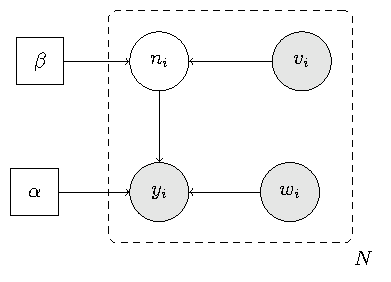
\includegraphics[width=0.5\textwidth]{figuras/modelo_v2.pdf}
        \caption{Representación gráfica del modelo pogit. Los círculos indican variables aleatorias y las flechas indican dependencia condicional. Los nodos sombreados representan cantidades observadas.}
        \label{fig:pogit}
    \end{figure}





















    \section{Antecedentes}
\label{sec:antecedentes}

La estimación del \emph{Size--of--Wallet} (SioW) y de la \emph{Share--of--Wallet} (SoW) constituye un eje central en la literatura de marketing relacional y analítica de clientes desde finales de la década de 1990. En este cuerpo de trabajo se reconoce que la evaluación del valor económico de un cliente no puede basarse únicamente en el gasto observado en una empresa específica, sino que debe considerar el volumen total de consumo del cliente dentro de una categoría y la proporción de dicho gasto que es capturada por una firma particular. En este marco, el SioW se define como el gasto total del cliente en la categoría, independientemente del proveedor, mientras que la SoW representa la fracción de ese gasto asignada a la empresa focal \cite{du2007size,glady2009predicting}.

Esta distinción resulta fundamental para la gestión estratégica de clientes, ya que un cliente con alto nivel de compras en la empresa focal no necesariamente presenta una alta SoW, y, de manera análoga, un cliente con una SoW elevada puede corresponder a un consumidor de bajo volumen total en la categoría. Trabajos como los de \cite{du2007size} formalizan esta separación conceptual y muestran que la identificación de clientes con alto potencial de crecimiento requiere distinguir entre tamaño absoluto de la billetera y grado de fidelidad relativa hacia la empresa.

En paralelo, diversos estudios han cuestionado la suficiencia de indicadores tradicionales como la satisfacción o el \emph{Net Promoter Score} para explicar el comportamiento económico real de los clientes. En particular, \cite{Keiningham2011} documentan que variaciones modestas en la SoW pueden generar impactos financieros sustancialmente mayores que cambios comparables en medidas de satisfacción declarada, lo que ha impulsado un creciente interés por metodologías cuantitativas orientadas a estimar la SoW de forma directa o indirecta.

Una primera familia de enfoques para estimar SioW y SoW se basa en la recolección directa de información mediante encuestas, paneles de consumidores o diarios de compra. Estos métodos permiten aproximar el gasto total del cliente y su distribución entre marcas o proveedores, proporcionando una referencia cercana al concepto teórico de wallet \cite{du2007size}. No obstante, la literatura reconoce importantes limitaciones prácticas asociadas a estos enfoques, entre las que se incluyen altos costos de implementación, sesgos de memoria y deseabilidad social, baja escalabilidad y dificultades para su integración con bases transaccionales empresariales. Estas limitaciones se acentúan en contextos B2B, donde los procesos de compra suelen ser complejos, agregados y altamente heterogéneos.

Como respuesta a estas restricciones, una segunda línea de investigación ha desarrollado metodologías que infieren el SioW y la SoW utilizando exclusivamente información transaccional y de perfilamiento disponible internamente en las organizaciones. En este grupo se incluyen modelos econométricos y estadísticos que emplean historiales de compra, frecuencias, montos, recencia y características estructurales del cliente para aproximar el comportamiento económico total en la categoría \cite{du2007size}. Estos enfoques reconocen explícitamente que las empresas observan únicamente una fracción del comportamiento real del cliente y buscan inferir la parte no observada a partir de patrones sistemáticos en los datos disponibles.

Dentro de esta familia, una contribución particularmente influyente es la propuesta de \cite{glady2009predicting}, quienes introducen un modelo pogit que separa conceptualmente dos mecanismos latentes: uno asociado al tamaño total de la billetera del cliente en la categoría y otro relacionado con la asignación de dicha billetera hacia la empresa focal. Este enfoque permite modelar de manera explícita la diferencia entre clientes con alta demanda total y clientes con alta propensión a asignar su gasto a una firma específica, utilizando conjuntos diferenciados de covariables transaccionales y de perfilamiento.

La relevancia del modelo de \cite{glady2009predicting} radica en su adecuación a contextos de información parcial, en los cuales no se dispone de la estimación de SoW como input para el modelo. El modelo se construye exclusivamente a partir de transacciones observadas por la empresa focal y permite inferir simultáneamente la SoW y el SioW como variables latentes, lo cual resulta especialmente apropiado para aplicaciones empresariales reales. Además, la separación explícita entre variables transaccionales y variables de perfilamiento proporciona una interpretación económica clara y coherente de los factores que influyen en cada componente del comportamiento del cliente.

De manera complementaria, la literatura en marketing ha desarrollado marcos conceptuales alternativos para explicar la SoW, como la \emph{Wallet Allocation Rule} (WAR) propuesta por \cite{keiningham2015wallet}. Este enfoque enfatiza el carácter multimarca del consumo y plantea que la distribución del gasto entre proveedores depende del posicionamiento relativo de cada marca en la mente del consumidor y del número total de marcas utilizadas. Si bien la WAR se apoya típicamente en información declarativa que no está disponible en la aplicación empírica de este trabajo, su aporte conceptual resulta relevante al reforzar la idea de que la SoW emerge de un proceso de asignación del gasto entre múltiples alternativas, proceso que puede manifestarse indirectamente en patrones transaccionales observables.

Finalmente, la literatura reporta el uso de modelos clásicos de conteo y técnicas de \emph{machine learning} —como árboles de decisión, \emph{random forests} y métodos de \emph{boosting}— para predecir montos de compra o clasificar clientes según niveles de SoW. No obstante, estos enfoques suelen tratar la SoW como una variable observada o exógena y no modelan explícitamente la estructura latente del wallet total del cliente, lo que limita su interpretación en entornos de información incompleta \cite{glady2009predicting}.

En síntesis, el presente trabajo se inscribe en la línea metodológica que busca inferir simultáneamente el tamaño y la asignación de la billetera del cliente a partir de datos transaccionales parciales. Siguiendo el enfoque de \cite{glady2009predicting}, y complementándolo con técnicas de reducción de dimensionalidad y segmentación exploratoria, este estudio adapta dichos modelos al contexto específico de clientes empresariales de una empresa distribuidora de biblias y literatura cristiana, proporcionando una base metodológica sólida para el análisis económico y la toma de decisiones estratégicas en ausencia de información proveniente de encuestas o transacciones con competidores.


     % --------------------------
    \chapter{Datos}
        El proyecto se desarrolló a partir de la base de datos transaccional de la Sociedad Bíblica Colombiana (SBC), la cual consolida información detallada de ventas a nivel de línea de factura para los años 2022, 2023 y 2024. Cada registro corresponde a una línea individual de venta e incluye información del cliente, del producto adquirido y de las condiciones comerciales asociadas a la operación.

La base de datos original contiene un total de 106{,}254 registros a nivel de línea de factura e integra información tanto de clientes personas naturales como de clientes empresariales. En una etapa posterior del análisis, el estudio se restringe al subconjunto de clientes empresariales, dado que el objetivo del trabajo es modelar el comportamiento de compra de este segmento específico. No obstante, en esta sección se describe la estructura completa de la base de datos tal como es recibida originalmente, antes de aplicar filtros por tipo de cliente o procesos de agregación.

A nivel de contenido, cada registro incluye identificadores del cliente, características del producto (como SKU, grupo, clase y subclase), variables monetarias (valor bruto, descuentos aplicados, valor neto, costos y utilidad), información geográfica (país, departamento y ciudad de la compra) y atributos comerciales relevantes (tipo de factura, condición de pago y categoría del producto). Esta estructura permite reconstruir el historial transaccional de cada cliente y constituye el insumo fundamental para las etapas posteriores de limpieza, agregación y construcción de variables analíticas.
En la Tabla~\ref{tab:tab-variables-originales} se presenta un resumen de las principales variables contenidas en la base de datos original. 


\begin{table}[H]
\centering
\small
\caption{Variables contenidas en la base de datos transaccional original de la SBC.}
\label{tab:tab-variables-originales}
\renewcommand{\arraystretch}{1.25} 
\begin{tabular}{c l c p{6.2cm}} 
\hline
\textbf{No.} & \textbf{Nombre de la variable} & \textbf{Notación} & \textbf{Descripción} \\ \hline

1  & Valor bruto           
   & VB 
   & Valor total del producto antes de aplicar descuentos, registrado a nivel de línea de factura. \\

2  & Descuento             
   & DS 
   & Descuento aplicado al valor bruto del producto en la línea de factura. \\

3  & Valor neto            
   & VN
   & Valor final pagado por el cliente una vez aplicado el descuento sobre el valor bruto. \\

4  & Costo total           
   & CT
   & Costo directo incurrido por la SBC para producir o adquirir el producto vendido. \\

5  & Utilidad bruta        
   & UB
   & Diferencia entre el valor neto y el costo total del producto en la línea de factura. \\

6  & Código de cliente     
   & CC
   & Identificador numérico único del cliente, generado por la SBC. \\

7  & Tipo de empresa       
   & TE
   & Clasificación del cliente empresarial (editorial, fundación, institución religiosa, comercial, entre otros). \\

8  & Mes                  
   & MS
   & Mes calendario en el que se registró la transacción. \\

9  & País                 
   & PA
   & País donde se realizó la compra. \\

10 & Departamento          
   & DP
   & Departamento asociado a la ciudad donde se efectuó la compra. \\

11 & Ciudad               
   & CI
   & Ciudad donde fue realizada la transacción. \\

12 & Tipo de factura      
   & TF
   & Tipo de documento de facturación que define la modalidad comercial de la venta (por ejemplo, nacional o exterior). \\

13 & Grupo                
   & GR
   & Grupo de producto al que pertenece el artículo vendido. \\

14 & Clase                
   & CL
   & Clasificación específica del producto dentro del grupo correspondiente. \\

15 & Clase 2              
   & C2
   & Agrupación general derivada de la descripción del producto (por ejemplo, BIBLIAS). \\

16 & Tamaño               
   & TM
   & Tamaño o formato del producto adquirido. \\

17 & SKU                  
   & SKU
   & Código único que identifica el producto dentro del inventario de la SBC. \\

18 & Condición            
   & CD
   & Condición de pago asociada a la transacción (contado, crédito, anticipado, entre otros). \\

19 & Categoría            
   & CAT
   & Clasificación del producto según su nivel de calidad (económica, línea, semifina, fina, etc.). \\

\hline
\end{tabular}
\end{table}

     
     % --------------------------
    \chapter{Metodología}
        

%--------------------------------------------------
\section{Limpieza, filtrado y reglas explícitas}
    Con el fin de garantizar la consistencia interna de la base de datos y la validez de los análisis posteriores, se aplicó un conjunto de reglas explícitas de limpieza y filtrado sobre los registros transaccionales originales. Estas reglas se definieron ex ante y se aplicaron de manera sistemática, con el objetivo de asegurar la trazabilidad y reproducibilidad del proceso de preparación de datos.

    En primer lugar, se excluyeron todas las observaciones asociadas a devoluciones, notas crédito o anulaciones, identificadas a partir del tipo de documento registrado en la variable \texttt{TIPO\_FACT} (por ejemplo, \texttt{NC}, \texttt{DEV} y categorías equivalentes). Esta exclusión responde a la necesidad de trabajar exclusivamente con transacciones que representen ventas efectivas, evitando que operaciones de reversión distorsionen las magnitudes económicas analizadas.
    
    En una segunda etapa, se realizó un diagnóstico sistemático de registros duplicados utilizando como clave la combinación de \texttt{COD\_CLIENTE}, \texttt{NUM\_FACT} y \texttt{LINEA}. Cuando los duplicados correspondían a fragmentaciones de un mismo registro transaccional, estos se consolidaron mediante la suma de los montos asociados. En contraste, los duplicados exactos se eliminaron conservando una única observación. Las reglas aplicadas en cada caso se documentaron de manera explícita para garantizar la trazabilidad del procedimiento.
    
    Adicionalmente, se identificaron y eliminaron aquellas filas que carecían de un identificador válido de cliente (\texttt{COD\_CLIENTE}), dado que la ausencia de este campo impide la correcta asignación de las transacciones a unidades de análisis a nivel individual.
    
    Finalmente, se verificó la validez de las fechas registradas en las transacciones. Este procedimiento incluyó la corrección de formatos inconsistentes y la eliminación de observaciones con fechas imposibles de interpretar o ubicadas fuera de un rango temporal razonable para el estudio.
    
    Cabe señalar que las reglas descritas en esta sección corresponden exclusivamente a procedimientos de depuración estructural y validación básica de los registros transaccionales originales. Estas etapas se aplican con anterioridad a cualquier transformación estadística, construcción de variables o decisión de modelamiento, las cuales se describen en secciones posteriores.

%--------------------------------------------------
\section{Identificación de datos faltantes}
    Como parte del proceso de validación y preparación de los datos, se definió un procedimiento sistemático para evaluar la presencia de valores faltantes en todas las variables consideradas para el análisis. Esta verificación se realizó a nivel de columna y de observación, con el objetivo de determinar la necesidad de aplicar técnicas de imputación o de exclusión de registros.

    El diagnóstico de datos faltantes se aplicó una vez concluido el proceso de limpieza y filtrado estructural, y abarcó tanto las variables transaccionales como las variables de perfilamiento del cliente y las magnitudes monetarias utilizadas posteriormente en la construcción de la variable respuesta del modelo \emph{pogit}.
    
    En caso de detectarse valores faltantes, el diseño metodológico contemplaba la aplicación de reglas explícitas de imputación o exclusión, debidamente documentadas. No obstante, cuando el diagnóstico no evidencia la presencia de datos faltantes, se evita la introducción de supuestos adicionales asociados a mecanismos de datos incompletos, preservando así la simplicidad y coherencia del pipeline de preprocesamiento.
    

%--------------------------------------------------
\section{Ventanas temporales y partición de los datos en conjuntos de entrenamiento y prueba}

    Es importante destacar que la definición de las ventanas temporales y la partición en conjuntos de entrenamiento y prueba cumplen roles conceptualmente distintos dentro del diseño metodológico. Las ventanas temporales \(T_1\) y \(T_2\) determinan \emph{qué información} se utiliza para la construcción de las variables predictoras y de la variable respuesta, respectivamente, mientras que la partición en entrenamiento y prueba define \emph{sobre qué clientes} se ajusta el modelo y se evalúan sus estimaciones fuera de muestra. En consecuencia, tanto el conjunto de entrenamiento como el conjunto de prueba contienen observaciones en ambas ventanas temporales: en \(T_1\), ambos conjuntos se utilizan para la construcción de predictores, y en \(T_2\), ambos conjuntos se emplean para la definición de la variable respuesta, manteniendo siempre una separación estricta entre los datos utilizados para el aprendizaje de parámetros y aquellos reservados para la evaluación estructural fuera de muestra.

    El diseño muestral y de modelamiento se estructura a partir de dos ventanas temporales no superpuestas, definidas con el objetivo de garantizar una separación estricta entre la información utilizada para la construcción de variables predictoras y aquella empleada para la evaluación del modelo. En particular, se define una \emph{ventana de características} \(T_{1}\), que abarca el periodo comprendido entre el 1 de enero de 2022 y el 31 de diciembre de 2023, y una \emph{ventana de respuesta o evaluación} \(T_{2}\), correspondiente al intervalo entre el 1 de enero de 2024 y el 31 de diciembre de 2024.
    
    Las variables predictoras del modelo se construyen exclusivamente a partir de la información observada durante \(T_{1}\). Estas incluyen medidas agregadas de comportamiento transaccional (RFM), intensidades por categoría, señales derivadas del historial de compra y atributos estructurales del cliente. La variable respuesta del modelo se define únicamente a partir de las transacciones observadas en \(T_{2}\), garantizando así la ausencia de superposición temporal entre predictores y respuesta.
    
    Con el fin de asegurar que las magnitudes latentes de asignación e intensidad estén bien definidas, la muestra analítica se restringe a aquellos clientes que realizaron al menos una compra a la empresa focal durante la ventana \(T_{1}\). Esta restricción define la cohorte de análisis sobre la cual se desarrolla el proceso de modelamiento.
    
    Sobre dicha cohorte, se establece una partición aleatoria a nivel de identificador de cliente en dos subconjuntos disjuntos: un conjunto de entrenamiento, que contiene el 70\% de los clientes, y un conjunto de prueba, que agrupa el 30\% restante. Esta partición se define \emph{ex ante} y se mantiene fija a lo largo de todo el proceso metodológico.
    
    Todos los procedimientos que implican aprendizaje a partir de los datos —incluyendo la construcción de transformaciones, la estandarización de variables, el tratamiento de valores extremos y la estimación del modelo \emph{pogit}— se realizan exclusivamente utilizando el conjunto de entrenamiento. El conjunto de prueba se reserva para el análisis posterior de las estimaciones fuera de muestra.
    
%--------------------------------------------------
\section{Construcción de variables predictoras}

    Los registros transaccionales depurados se consolidan en una matriz a nivel de cliente, con una fila por cliente y columnas correspondientes a las variables predictoras construidas a partir de la información observada durante la ventana de características \(T_1\). La muestra analítica se restringe a clientes que realizaron al menos una compra a la Empresa Distribuidora de Literatura Cristiana durante dicha ventana, con el fin de garantizar que las variables transaccionales específicas de la empresa focal, utilizadas en el componente de asignación del modelo, estén bien definidas.
    
    Las variables categóricas incluidas como predictores se codifican mediante esquemas \emph{one--hot}, eliminando un nivel de referencia por factor con el objetivo de evitar problemas de colinealidad e identificar de manera adecuada los parámetros del modelo. Este procedimiento se aplica a atributos estructurales del cliente, tales como ubicación geográfica, tipo de empresa, categoría de producto y condiciones comerciales.
    
    Para capturar la heterogeneidad en el componente de asignación del gasto (\emph{Share--of--Wallet}), se construyen las variables del esquema clásico RFM (\emph{Recency, Frequency, Monetary}) de manera específica para la empresa focal. La frecuencia corresponde al número de transacciones realizadas por el cliente durante \(T_1\); la variable monetaria se define como la suma del valor total de los ítems adquiridos, calculada como \(\textit{precio\_unitario} \times \textit{cantidad}\), neta de descuentos a nivel de producto y excluyendo impuestos y costos de envío; la recencia se mide como el número de días transcurridos entre la fecha final de \(T_1\) (31 de diciembre de 2023) y la fecha de la compra más reciente del cliente en dicho periodo.
    
    Todas las variables predictoras descritas en esta sección se construyen exclusivamente a partir de información observada durante la ventana \(T_1\). Ninguna información proveniente de la ventana de evaluación \(T_2\) interviene en su definición, garantizando la ausencia de fuga de información entre las etapas de construcción de predictores y estimación del modelo.
    
%--------------------------------------------------
\section{Construcción de la variable respuesta}
    Siguiendo a \cite{glady2009predicting}, cuando se observan volúmenes monetarios de gasto, estos pueden discretizarse en unidades tipo conteo antes de la estimación. En esta aplicación, se utiliza el gasto del cliente \(i\) en libros y revistas cristianas adquiridos a la Empresa Distribuidora de Literatura Cristiana dentro del universo de productos \(\mathcal{U}\) durante la ventana de evaluación \(T_2\), el cual se denota por
    \[
    \mathrm{spend}_{i}^{\mathrm{EDLC}\mid\mathrm{focal},\mathcal{U}}.
    \]
    
    Con el fin de evitar fuga de información, todas las cantidades necesarias para determinar la escala de discretización se calculan exclusivamente utilizando los clientes del conjunto de entrenamiento. Sea \(\mathcal{I}_{\mathrm{tr}}\) el conjunto de índices de los clientes de entrenamiento, con tamaño \(N_{\mathrm{tr}} = |\mathcal{I}_{\mathrm{tr}}|\). La media y la varianza muestral del gasto en la empresa focal dentro del conjunto de entrenamiento se definen como
    \begin{align*}
    \overline{\mathrm{spend}}_{\mathrm{tr}}^{\mathrm{EDLC}\mid\mathrm{focal},\mathcal{U}}
    &=
    \frac{1}{N_{\mathrm{tr}}}\sum_{j\in\mathcal{I}_{\mathrm{tr}}}
    \mathrm{spend}_{j}^{\mathrm{EDLC}\mid\mathrm{focal},\mathcal{U}},\\[0.5em]
    \widehat{\sigma}^2_{\mathrm{tr}}{}^{\mathrm{EDLC}\mid\mathrm{focal},\mathcal{U}}
    &=
    \frac{1}{N_{\mathrm{tr}}-1}\sum_{j\in\mathcal{I}_{\mathrm{tr}}}
    \Bigl(
    \mathrm{spend}_{j}^{\mathrm{EDLC}\mid\mathrm{focal},\mathcal{U}}
    -
    \overline{\mathrm{spend}}_{\mathrm{tr}}^{\mathrm{EDLC}\mid\mathrm{focal},\mathcal{U}}
    \Bigr)^2.
    \end{align*}
    
    A diferencia de \cite{glady2009predicting}, se define la constante de discretización como el cociente entre la varianza y la media del gasto transversal en el conjunto de entrenamiento,
    \[
    c
    =
    \frac{
    \widehat{\sigma}^2_{\mathrm{tr}}{}^{\mathrm{EDLC}\mid\mathrm{focal},\mathcal{U}}
    }{
    \overline{\mathrm{spend}}_{\mathrm{tr}}^{\mathrm{EDLC}\mid\mathrm{focal},\mathcal{U}}
    },
    \]
    lo cual está motivado por la suposición Poisson subyacente en el componente de intensidad del modelo, según la cual la media y la varianza coinciden en la escala del modelo.

    Es importante señalar que el tratamiento de valores extremos descrito a continuación se aplica \emph{exclusivamente} a la variable de gasto utilizada para la construcción de la variable respuesta \(y_i\). Este procedimiento tiene como único objetivo estabilizar la estimación de la constante de discretización \(c\) y no forma parte del preprocesamiento general de las covariables del modelo. El tratamiento de valores extremos aplicado posteriormente a las variables predictoras se describe de manera independiente en la subsección de Preprocesamiento.

    Antes de calcular la constante \(c\), los valores extremos del gasto en la Empresa Distribuidora de Literatura Cristiana durante \(T_2\) se tratan en dos etapas. En primer lugar, se eliminan un número reducido de observaciones severamente anómalas mediante una regla de Tukey extrema definida a nivel de aplicación (\(k = 5\)). En segundo lugar, la cola superior de la distribución se winsoriza utilizando una regla de Tukey con \(k = 3\). Para evitar fuga de información, tanto los umbrales de eliminación como los de winsorización se estiman exclusivamente a partir del conjunto de entrenamiento y luego se aplican sin modificaciones al conjunto de prueba. La constante de discretización \(c\) se calcula únicamente a partir del gasto del conjunto de entrenamiento una vez filtrado y winsorizado, y se mantiene fija en todas las etapas posteriores del análisis.
    
    La variable respuesta del modelo se define entonces como
    \[
    y_i
    =
    \operatorname{round}\!\left(
    \frac{\mathrm{spend}_{i}^{\mathrm{EDLC}\mid\mathrm{focal},\mathcal{U}}}{c}
    \right),
    \]
    y debe interpretarse como un \emph{proxy normalizado y discretizado del gasto}, no como un conteo literal de unidades, pedidos o transacciones.
    
    Con fines estrictamente interpretativos, se introduce la noción de un \emph{proxy empírico} del tamaño de la billetera en la categoría, el cual solo podría construirse en un escenario ideal en el que se dispusiera de información completa sobre el gasto del cliente en todas las distribuidoras de libros y revistas cristianas, y no únicamente en la empresa focal. En dicha situación hipotética, este proxy se definiría como
    \[
    n_i^{\mathrm{emp}}
    =
    \operatorname{round}\!\left(
    \frac{\mathrm{spend}_{i}^{\mathcal{U}}}{c}
    \right),
    \]
    donde \(\mathrm{spend}_{i}^{\mathcal{U}}\) denota el gasto total del cliente \(i\) en libros y revistas cristianas dentro del universo \(\mathcal{U}\) durante la ventana \(T_2\).
    
    En la aplicación considerada en este trabajo, \(\mathrm{spend}_{i}^{\mathcal{U}}\) no es observable, por lo que \(n_i^{\mathrm{emp}}\) no puede calcularse y no se utiliza en ninguna etapa del análisis empírico. Su inclusión aquí tiene únicamente un propósito conceptual: clarificar la interpretación de la variable latente \(n_i\) del modelo \emph{pogit}. En particular, \(n_i\) debe entenderse como el tamaño total de la billetera del cliente en la categoría, expresado en la misma escala normalizada y discretizada que la variable observada \(y_i\). Bajo esta interpretación, el modelo vincula un proxy observable del gasto en la empresa focal (\(y_i\)) con un volumen total latente en la categoría (\(n_i\)), aun cuando este último no pueda observarse directamente. Este proxy hipotético no forma parte de la función de verosimilitud ni del proceso de estimación del modelo \emph{pogit}.

    Esta construcción permite compatibilizar datos monetarios continuos con un marco de conteo discreto, manteniendo coherencia con los supuestos del modelo pogit.

%--------------------------------------------------
\section{Análisis exploratorio}
    Una vez completadas las etapas de limpieza, validación y construcción de variables, se realizó un análisis exploratorio de los datos con el objetivo de caracterizar las distribuciones de las variables, identificar patrones relevantes y apoyar las decisiones de selección y depuración de covariables para el modelo \emph{pogit}. Esta etapa se concibió como un análisis diagnóstico previo al modelamiento, orientado a garantizar la estabilidad e interpretabilidad de los resultados.
    
    Para las variables cuantitativas, se calcularon medidas de tendencia central y dispersión, así como la proporción de valores atípicos. Adicionalmente, se construyeron histogramas y diagramas de caja para examinar la forma de las distribuciones y detectar posibles asimetrías o colas largas que pudieran afectar la estimación de los componentes del modelo. En el caso de las variables categóricas, se analizaron las frecuencias absolutas y relativas de cada categoría, con el fin de identificar concentraciones excesivas o niveles con baja representatividad.
    
    Posteriormente, se evaluó el grado de asociación entre variables cuantitativas mediante el coeficiente de correlación de Spearman y entre variables cualitativas mediante el estadístico de Cramér. Estos análisis se utilizaron como insumo para identificar redundancias entre covariables y apoyar decisiones de depuración, con el propósito de evitar problemas de multicolinealidad en la estimación del modelo.
    
    De manera complementaria, se analizó la distribución del gasto y de los precios por categoría de producto, así como la concentración de clientes en cada una de ellas, con el objetivo de comprender la estructura del portafolio atendido por la Empresa Distribuidora de Literatura Cristiana. Asimismo, se examinó la relación entre los descuentos otorgados y el monto total gastado por los clientes; este análisis no evidenció una asociación sistemática, por lo que dichas variables se consideraron únicamente desde una perspectiva descriptiva.
    
    Finalmente, con base en los resultados del análisis exploratorio, se depuró el conjunto de variables predictoras eliminando o ajustando aquellas cuya correlación superaba el umbral de 0.70. Esta decisión permitió reducir redundancias y mejorar la estabilidad numérica y la interpretabilidad de los componentes de asignación (SoW) e intensidad (SioW) del modelo.

    El análisis exploratorio permite caracterizar de manera descriptiva la estructura de las variables predictoras construidas a partir de la ventana \(T_1\). Los resultados muestran distribuciones altamente asimétricas, presencia significativa de valores extremos y una marcada heterogeneidad transversal entre clientes empresariales, así como patrones claros de concentración por tipo de empresa, categoría de producto y localización geográfica.
%--------------------------------------------------
%--------------------------------------------------
\section{Preprocesamiento}

    Con el fin de evitar fuga de información, todos los pasos de preprocesamiento que dependen de los datos se estiman exclusivamente a partir del conjunto de clientes de entrenamiento y posteriormente se aplican sin modificaciones al conjunto de prueba retenido. La partición entre entrenamiento y prueba se realiza a nivel de identificador de cliente, garantizando que todas las observaciones asociadas a un mismo cliente pertenezcan al mismo conjunto.
    
    El preprocesamiento se estructura en cuatro etapas secuenciales: (i) tratamiento de valores extremos en variables cuantitativas, (ii) análisis de asociación y depuración de covariables cuantitativas y cualitativas, (iii) codificación de variables categóricas y (iv) estandarización de variables continuas. Este orden responde a criterios de estabilidad numérica, identificabilidad del modelo y coherencia con los supuestos del modelo \emph{pogit}.

\subsection{Tratamiento de valores extremos en variables cuantitativas}

    Las variables cuantitativas fueron sometidas a un tratamiento de valores extremos con el objetivo de mitigar la influencia de observaciones severamente anómalas sobre las etapas posteriores de análisis y modelamiento. En particular, se aplicó un procedimiento en dos fases: (i) eliminación de observaciones extremadamente atípicas utilizando una regla de Tukey con umbral $k = 5$, y (ii) winsorización de la cola superior de la distribución mediante una regla de Tukey con $k = 3$.
    
    Los umbrales correspondientes se estimaron exclusivamente a partir del conjunto de entrenamiento y se aplicaron sin modificación al conjunto de prueba, preservando así la separación temporal y evitando la incorporación de información futura en el proceso de aprendizaje.

\subsection{Análisis de asociación y depuración de variables cuantitativas}

    Una vez controlado el efecto de valores extremos, se evaluó el grado de asociación entre las variables cuantitativas predictoras con el objetivo de identificar redundancias informativas y reducir problemas de multicolinealidad en el modelo. Para este fin, se empleó el coeficiente de correlación de Spearman, dado su carácter no paramétrico y su robustez frente a distribuciones asimétricas y colas pesadas, típicas de datos transaccionales empresariales.
    
    Las correlaciones se calcularon exclusivamente sobre el conjunto de entrenamiento y se adoptó un umbral fijo de $|\rho| \geq 0.70$ para identificar asociaciones fuertes. 
    Este umbral se adopta como un criterio operativo conservador, comúnmente utilizado en análisis exploratorio, orientado a identificar redundancias sustantivas sin eliminar relaciones moderadas que pueden aportar información complementaria al modelo.


\subsection{Análisis de asociación y depuración de variables cualitativas}

    De manera complementaria, se evaluó la asociación entre variables cualitativas mediante el estadístico V de Cramér, el cual es apropiado para medir la intensidad de asociación entre variables categóricas nominales y ordinales. Dado que los valores de este estadístico suelen ser moderados incluso en presencia de relaciones estructuralmente fuertes, se adoptó un umbral conservador de $V \geq 0.50$ para identificar redundancias sustantivas.
    
    Este análisis permitió detectar jerarquías y solapamientos entre variables categóricas asociadas a dimensiones similares del comportamiento del cliente (por ejemplo, estructura del producto, localización geográfica u origen de la transacción). En presencia de asociaciones elevadas, se conservó la variable que ofrecía un mayor equilibrio entre capacidad explicativa, interpretabilidad económica y control de la dimensionalidad del modelo, excluyendo las restantes.
    
\subsection{Codificación de variables categóricas}

    Las covariables categóricas de selección única retenidas tras el proceso de depuración se codificaron mediante variables indicadoras (\emph{dummies}), omitiendo un nivel de referencia por factor con el fin de garantizar la identificabilidad de los parámetros del modelo. En el caso de constructos de selección múltiple, cada categoría se codificó como un indicador binario independiente, dado que dichas categorías pueden coexistir para un mismo cliente.

\subsection{Estandarización de variables cuantitativas}

    Finalmente, las variables cuantitativas seleccionadas tras el proceso de depuración se estandarizaron utilizando las medias y desviaciones estándar calculadas exclusivamente sobre el conjunto de entrenamiento. Los mismos parámetros de centrado y escalamiento se aplicaron posteriormente al conjunto de prueba.
    
    Este paso es necesario para garantizar que todas las covariables continuas contribuyan de manera comparable en procedimientos sensibles a la escala, como el análisis de componentes principales (PCA), los algoritmos de segmentación exploratoria y la estimación del modelo \emph{pogit}. La estandarización no altera las relaciones ordinales entre observaciones ni introduce información futura, y constituye la base común para las etapas posteriores de reducción de dimensionalidad y modelamiento.

%--------------------------------------------------
\section{Construcción de matrices de diseño del modelo \emph{pogit}}

    En esta sección se describe la construcción de las matrices de diseño utilizadas en la estimación del modelo \emph{pogit}. De acuerdo con la estructura conceptual del modelo, se definen dos matrices de covariables con funciones claramente diferenciadas: la matriz $\mathbf{W}$, asociada al mecanismo de asignación del gasto y, por tanto, al componente de \emph{Share--of--Wallet} (SoW), y la matriz $\mathbf{V}$, vinculada al mecanismo de intensidad latente de consumo y al componente de \emph{Size--of--Wallet} (SioW).
    
    La matriz $\mathbf{W}$ se construye a partir de variables transaccionales directamente observadas y resume distintos aspectos del comportamiento de compra de cada cliente. En particular, incluye medidas del tipo RFM (\emph{recency, frequency, monetary}), así como otros indicadores cuantitativos derivados de las transacciones que capturan la intensidad, recurrencia y magnitud económica de la relación comercial entre el cliente y la empresa focal. Adicionalmente, se incorporan en $\mathbf{W}$ aquellas denominadas \emph{condiciones del cliente} —por ejemplo, consignación, crédito o distribución— únicamente en la medida en que representan modalidades operativas directamente asociadas al comportamiento transaccional, y no como atributos estructurales del perfil del cliente.
    
    Con el fin de garantizar condiciones adecuadas de diseño del modelo, las variables candidatas a integrar la matriz $\mathbf{W}$ son sometidas previamente a un proceso sistemático de preprocesamiento y selección. En este proceso, las asociaciones entre variables cuantitativas se evalúan mediante el coeficiente de correlación de Spearman, mientras que las asociaciones entre variables categóricas se analizan utilizando el estadístico $V$ de Cramér. Estos análisis no tienen un propósito inferencial, sino que se emplean exclusivamente como criterios operativos para identificar redundancias informativas y reducir problemas de multicolinealidad, sobreparametrización e inestabilidad numérica en la estimación del modelo.
    
    Sobre la base de estos criterios, se define una primera especificación de la matriz $\mathbf{W}$ construida directamente a partir de un subconjunto parsimonioso de variables transaccionales originales. Esta especificación conserva la interpretación económica directa de las medidas RFM y de los indicadores transaccionales seleccionados, y constituye la referencia principal para la estimación del componente de asignación del modelo \emph{pogit}.
    
    Adicionalmente, se considera una segunda especificación alternativa de la matriz $\mathbf{W}$, obtenida mediante un Análisis de Componentes Principales (PCA) aplicado exclusivamente a las variables transaccionales cuantitativas previamente estandarizadas. El PCA se utiliza como un mecanismo de reducción de dimensionalidad que permite sintetizar la información contenida en variables potencialmente correlacionadas, manteniendo una proporción sustancial de la variabilidad total de los datos. En particular, se retienen aquellas componentes principales que, en conjunto, explican al menos el 70\% de la variabilidad total. Las variables categóricas codificadas mediante indicadores no se incluyen en el procedimiento de PCA y se incorporan de manera separada en la matriz de diseño.
    
    Esta segunda especificación se introduce como una alternativa parsimoniosa para representar la información transaccional sin alterar la interpretación conceptual de la matriz $\mathbf{W}$, y permite evaluar la robustez de las inferencias del modelo \emph{pogit} frente a distintas representaciones del comportamiento de compra. Las componentes principales definidas en esta etapa constituyen, además, el insumo básico para las técnicas de reducción de dimensionalidad y segmentación exploratoria presentadas en la sección siguiente.
    
    Por su parte, la matriz $\mathbf{V}$ contiene exclusivamente variables de perfilamiento del cliente o de la empresa, las cuales describen características estructurales y contextuales relativamente estables en el tiempo. Estas variables incluyen, entre otras, el tipo de empresa, la localización geográfica y atributos generales del cliente o de la categoría de producto. Al igual que en el caso de la matriz $\mathbf{W}$, las covariables que integran $\mathbf{V}$ son sometidas a procesos de depuración y selección orientados a evitar redundancias y garantizar condiciones adecuadas de identificabilidad y estabilidad numérica del modelo.
    
    A diferencia de las variables incluidas en $\mathbf{W}$, las covariables de la matriz $\mathbf{V}$ no capturan intensidad ni recurrencia de compra, sino que introducen heterogeneidad transversal en el perfil de los clientes, permitiendo explicar diferencias sistemáticas en el tamaño de la billetera (SioW) dentro del marco del modelo \emph{pogit}. Las distintas combinaciones de $\mathbf{W}$ y $\mathbf{V}$ definidas en esta etapa dan lugar a un conjunto de especificaciones alternativas del modelo, que se implementan y comparan en la sección de resultados con el objetivo de evaluar la estabilidad estructural de las inferencias sobre SoW y SioW.

%--------------------------------------------------
\subsection{Reducción de dimensionalidad y segmentación exploratoria}
\label{sec:pca_segmentacion}

    Con el propósito de explorar la estructura subyacente de las variables transaccionales cuantitativas, caracterizar perfiles de clientes y apoyar la interpretación económica de los resultados del modelo \emph{pogit}, se emplearon técnicas de reducción de dimensionalidad y segmentación no supervisada. Estas herramientas cumplen un rol complementario dentro de la metodología: (i) el Análisis de Componentes Principales (PCA) se utiliza tanto con fines exploratorios como para definir una especificación alternativa y parsimoniosa de la matriz de covariables transaccionales $\mathbf{W}$, y (ii) los algoritmos de segmentación se emplean exclusivamente para la caracterización descriptiva de clientes y la evaluación estructural de las estimaciones del modelo, sin intervenir directamente en su proceso de estimación.
    
    En primer lugar, se aplicó un Análisis de Componentes Principales (PCA) sobre el conjunto completo de variables transaccionales cuantitativas construidas a partir de la ventana de características $T_1$. En particular, el PCA incluyó las siguientes variables: \textit{Recency}, \textit{Frequency}, \textit{Monetary}, \textit{Valor Bruto}, \textit{Valor Neto}, \textit{SKUs Distintos}, \textit{Descuentos}, \textit{Cantidad}, \textit{Costo Total} y \textit{Utilidad Bruta}. Todas las variables fueron previamente transformadas y estandarizadas de acuerdo con el esquema de preprocesamiento descrito en la sección metodológica, con el fin de garantizar comparabilidad en escala y evitar la dominancia de variables de mayor magnitud.
    
    La inclusión de este conjunto ampliado de variables permite capturar de manera integral distintas dimensiones del comportamiento económico del cliente, incluyendo la recurrencia de compra, la magnitud del gasto, la diversidad del portafolio adquirido, la estructura de costos y la política de descuentos. En este contexto, el PCA cumple una doble función metodológica. Por un lado, permite analizar empíricamente la estructura de dependencia y redundancia entre las variables cuantitativas. Por otro, define una representación alternativa y de menor dimensionalidad de la matriz $\mathbf{W}$ del modelo \emph{pogit}, en la cual las variables transaccionales originales son reemplazadas por un conjunto reducido de componentes ortogonales que preservan una proporción sustancial de la variabilidad total. En particular, se retuvieron aquellas componentes principales que, en conjunto, explican al menos el 70\% de la variabilidad total observada.
    
    De manera complementaria, se implementaron técnicas de segmentación no supervisada con el objetivo de identificar perfiles homogéneos de clientes y apoyar la interpretación estructural de las estimaciones del modelo \emph{pogit}. En este caso, el énfasis no se coloca en la reducción de dimensionalidad, sino en la identificación de agrupaciones basadas en información de naturaleza mixta, combinando variables cuantitativas y categóricas.
    
    En particular, se aplicó el algoritmo \emph{k-medoids} utilizando la distancia de Gower, lo cual permite integrar variables continuas y cualitativas dentro de una misma matriz de disimilitud. Para este procedimiento se consideraron como variables cuantitativas \textit{Monetary}, \textit{Frequency}, \textit{Recency} y \textit{Descuentos}, las cuales capturan dimensiones centrales del comportamiento transaccional del cliente. Adicionalmente, se incorporaron variables categóricas asociadas al contexto operativo y estructural del cliente, incluyendo el \textit{Tipo} de cliente, el \textit{Departamento}, la \textit{Categoría} de producto, el \textit{Tamaño} del producto, el \textit{Mes} de compra, el \textit{Tipo de Empresa} y la \textit{Condición} comercial.
    
    Esta diferenciación explícita en la selección de variables refleja los distintos objetivos metodológicos de cada técnica. Mientras que el PCA se orienta a la exploración de la estructura latente de las variables cuantitativas y a la definición de especificaciones alternativas de la matriz $\mathbf{W}$ del modelo \emph{pogit}, los algoritmos de segmentación se emplean exclusivamente con fines descriptivos e interpretativos. En consecuencia, los resultados de clustering no modifican el proceso de estimación del modelo \emph{pogit}, sino que se utilizan posteriormente para evaluar la coherencia, estabilidad e interpretabilidad económica de las estimaciones de \emph{Share--of--Wallet} y \emph{Size--of--Wallet}.

%--------------------------------------------------
\section{Estimación de SoW and SioW}

\subsubsection{Modelo}
    El modelo predice la \emph{participación en la billetera} (\emph{Share--of--Wallet}, SoW) de los clientes para la Empresa Distribuidora de Literatura Cristiana y su \emph{tamaño de la billetera} (\emph{Size--of--Wallet}, SioW) en la categoría de venta de libros y revistas, sin recurrir a datos de encuestas en las que los clientes reportan directamente sus participaciones de gasto.
    
    Suponemos la disponibilidad de una muestra
    \[
    \{(y_i, \boldsymbol{W}_i, \boldsymbol{V}_i, E_i)\}_{i=1}^N.
    \]
    En esta muestra, \(y_i\) denota un \emph{proxy} discretizado, de naturaleza similar a un conteo (expresado en una escala discreta por conveniencia modelística), construido a partir del gasto del cliente \(i\) en libros y revistas adquiridos a la Empresa Distribuidora de Literatura Cristiana, observado dentro del universo de venta de libros y revistas durante la ventana de evaluación. Es importante destacar que \(y_i\) se obtiene reescalando el gasto monetario mediante una constante \(c\) estimada en el conjunto de entrenamiento y posteriormente redondeando el resultado; por tanto, debe interpretarse como un proxy de gasto normalizado y no como un conteo literal de transacciones o de ejemplares adquiridos. La cantidad \(n_i\) representa el volumen total (latente) de compras del cliente en la categoría de libros y revistas, agregando todas las editoriales, distribuidoras y canales de venta, y expresado en la misma escala normalizada (discretizada) que \(y_i\).
    
    Los registros transaccionales disponibles corresponden exclusivamente a las compras realizadas a la Empresa Distribuidora de Literatura Cristiana; en consecuencia, las variables predictoras derivadas de transacciones se construyen únicamente a partir de esta información. Este esquema refleja de manera fiel el entorno informacional de una empresa focal, que típicamente observa solo las interacciones de sus clientes con su propio portafolio de productos y carece de información directa sobre las ventas de competidores o las compras efectuadas a través de otros canales. Precisamente, este tipo de estructura de información parcial es la que motiva el uso de modelos \emph{pogit}, los cuales permiten inferir el tamaño total de la billetera y la participación de gasto de la empresa focal a partir de datos transaccionales incompletos.
    
    El vector \(\boldsymbol{W}_i = (W_{ij}) \in \mathbb{R}^J\) contiene los \(J\) regresores asociados con el \emph{mecanismo de asignación} que gobierna la SoW del cliente \(i\) hacia la Empresa Distribuidora de Literatura Cristiana. Estas covariables corresponden a resúmenes transaccionales específicos de la empresa (por ejemplo, frecuencia de compra, diversidad de títulos adquiridos o regularidad del consumo) y capturan la variación en el comportamiento de asignación del gasto entre distintos proveedores de libros y revistas. De manera análoga, el vector \(\boldsymbol{V}_i = (V_{i\ell}) \in \mathbb{R}^L\) contiene los \(L\) regresores asociados con el \emph{mecanismo de intensidad}, el cual gobierna la demanda total del cliente en la categoría de libros y revistas (SioW).
    
    El escalar \(E_i > 0\) denota un \emph{offset} (o exposición) que captura diferencias exógenas en las oportunidades de compra, tales como el tiempo de permanencia del cliente en el mercado o su nivel de acceso a los puntos de venta. En el contexto empírico considerado, todos los clientes son observados durante la misma ventana temporal y se asume que enfrentan una exposición comparable. En consecuencia, se fija \(E_i \equiv 1\) para todo \(i\), de modo que la heterogeneidad transversal en la intensidad total de la categoría se modela completamente a través de las covariables en \(\boldsymbol{V}_i\) y del intercepto del componente de intensidad.
    
    El modelo se especifica jerárquicamente como
    \[
    \begin{aligned}
    y_i \mid n_i, \theta_i
    & \sim
    \mathrm{Bin}\!\left(n_i, \theta_i\right),
    \qquad
    i = 1, \ldots, N,
    \\
    n_i \mid \lambda_i
    & \sim
    \mathrm{Poisson}\!\left(\lambda_i\right),
    \\
    \log(\lambda_i)
    &=
    \log(E_i) + \boldsymbol{V}_i^{\prime}\boldsymbol{\beta}_2,
    \\
    \theta_i
    &=
    \operatorname{sigmoid}\!\left(\boldsymbol{W}_i^{\prime}\boldsymbol{\beta}_1\right),
    \end{aligned}
    \]
    donde \(\operatorname{sigmoid}(x) = \{1+\exp(-x)\}^{-1}\) denota la función sigmoide.
    
\subsubsection{Configuraciones alternativas de covariables y reducción de dimensionalidad}

    Dado que el modelo \emph{pogit} se estima bajo información transaccional parcial y que los componentes de asignación (\(\boldsymbol{W}_i\)) e intensidad (\(\boldsymbol{V}_i\)) representan procesos latentes conceptualmente distintos, la especificación empírica del modelo no se restringe a una única configuración de covariables. En su lugar, se consideran múltiples especificaciones alternativas con el objetivo de evaluar la estabilidad estructural de las inferencias sobre la participación en la billetera (SoW) y el tamaño de la billetera (SioW), así como la robustez de su interpretación económica frente a distintas representaciones del comportamiento del cliente.
    
    En particular, se exploran configuraciones en las que el componente de asignación \(\boldsymbol{W}_i\) se construye a partir de variables transaccionales originales del tipo RFM, y configuraciones alternativas en las que dichas variables se reemplazan por un conjunto reducido de componentes principales obtenidas mediante Análisis de Componentes Principales (PCA). La reducción de dimensionalidad se introduce exclusivamente en el componente de asignación, dado que este captura la estructura relativa de preferencias del cliente hacia la empresa focal, mientras que el componente de intensidad \(\boldsymbol{V}_i\) se mantiene especificado en términos de variables categóricas estructurales asociadas al perfil del cliente, la empresa y el contexto de compra.
    
    La incorporación de PCA no persigue mejorar el desempeño predictivo del modelo, sino evaluar si las inferencias sobre SoW se mantienen cuando el comportamiento transaccional se representa en un espacio latente de menor dimensión. De este modo, las componentes principales permiten sintetizar patrones económicos globales —como el tamaño relativo del cliente o la estructura de su gasto— y contrastar su efecto sobre la asignación del gasto frente a la empresa focal.
    
    De forma análoga, el componente de intensidad se estima bajo distintas configuraciones de \(\boldsymbol{V}_i\), incorporando subconjuntos alternativos de variables categóricas (por ejemplo, tipo de cliente, tipo de empresa, categoría de producto o estacionalidad), con el fin de capturar heterogeneidad estructural en el tamaño total de la billetera y evaluar su interacción con el componente de asignación.
    
    Este enfoque de especificaciones múltiples permite identificar una configuración de referencia del modelo \emph{pogit} que combine parsimonia, coherencia económica e interpretabilidad, y proporciona el marco metodológico para comparar de manera sistemática los resultados empíricos presentados en la sección de Resultados.


\subsection{Conjuntos de entrenamiento y prueba en modelos con variables latentes}
    En el aprendizaje estadístico, es habitual dividir la información disponible en un conjunto de entrenamiento y un conjunto de prueba con el fin de evaluar la estabilidad y el desempeño de los modelos estimados fuera de muestra. El conjunto de entrenamiento se utiliza para ajustar los parámetros del modelo y aprender las relaciones entre variables, mientras que el conjunto de prueba se reserva para analizar el comportamiento del modelo en observaciones no utilizadas durante la estimación.

    En modelos supervisados clásicos, esta evaluación suele realizarse comparando predicciones puntuales con valores observados de la variable respuesta. Sin embargo, en modelos con variables latentes —como el modelo Poisson--logístico (\emph{pogit})— esta lógica debe adaptarse. En este tipo de modelos, las cantidades de interés no son directamente observables, sino que se infieren a partir de la estructura probabilística del modelo y de los datos disponibles.

    En el modelo \emph{pogit}, tanto la probabilidad de asignación del gasto a la empresa focal como el tamaño total de la cartera del cliente corresponden a variables latentes. En consecuencia, no existe un valor empírico observado con el cual contrastar directamente las estimaciones fuera de muestra. Esta característica impide una validación predictiva tradicional basada en errores de predicción y requiere enfoques alternativos de evaluación.

    En consecuencia, en este estudio la validación del modelo \emph{pogit} no se concibe
    como un ejercicio de precisión predictiva puntual, sino como un proceso de validación
    estructural y conceptual, coherente con la naturaleza latente de las cantidades de
    interés. Esta validación se articula en torno a tres criterios complementarios:
    (i) coherencia interna de las estimaciones con la estructura probabilística del modelo;
    (ii) estabilidad de las inferencias frente a distintas configuraciones de covariables y
    representaciones del comportamiento del cliente; y (iii) consistencia estructural de
    las estimaciones fuera de muestra al contrastarlas con segmentaciones no supervisadas
    basadas en información observable.


\subsubsection{Estimaciones para los componentes de asignación  e intensidad}
    Esta subsección presenta cómo se estiman los dos mecanismos latentes del modelo \emph{pogit} en la aplicación a la Empresa Distribuidora de Literatura Cristiana: (i) el componente de \emph{asignación}, que gobierna la participación en la billetera (\emph{Share--of--Wallet}, SoW), y (ii) el componente de \emph{intensidad}, que gobierna el tamaño de la billetera (\emph{Size--of--Wallet}, SioW). Estos dos componentes representan procesos latentes conceptualmente distintos: el primero captura la probabilidad de que la demanda total en la categoría de libros y revistas cristianas se asigne a la empresa focal, mientras que el segundo describe la intensidad global de consumo del cliente en dicha categoría.
    
    El mecanismo de asignación se especifica como
    \[
    \theta_i 
    = 
    \operatorname{sigmoid}\!\left(\boldsymbol{W}_i' \boldsymbol{\beta}_1\right),
    \]
    de modo que los coeficientes \(\boldsymbol{\beta}_1\) actúan sobre los \emph{log--odds} de asignar el gasto de la categoría a la Empresa Distribuidora de Literatura Cristiana. En este contexto, coeficientes positivos incrementan,  la probabilidad de que el cliente destine una mayor fracción de su gasto en libros y revistas cristianas a la empresa focal, mientras que coeficientes negativos la reducen.
    
    En esta aplicación empírica de este estudio, la exposición se normaliza fijando \(E_i \equiv 1\), de manera que la intensidad \(\lambda_i\) depende exclusivamente de las covariables incluidas en \(\boldsymbol{V}_i\).
    
    Sea \(\hat{\boldsymbol{\beta}}_1\) y \(\hat{\boldsymbol{\beta}}_2\) los estimadores de los parámetros de los componentes de asignación e intensidad, respectivamente. Para cada cliente \(i = 1, \ldots, N\), las cantidades latentes ajustadas se obtienen como
    \begin{equation*}
    \begin{aligned}
    \hat{\theta}_i 
    &= 
    \operatorname{sigmoid}(\hat{\eta}_{i1}),
    &
    \hat{\eta}_{i1} 
    &= 
    \boldsymbol{W}_i' \hat{\boldsymbol{\beta}}_1,
    \\
    \hat{\lambda}_i 
    &= 
    \exp(\hat{\eta}_{i2}),
    &
    \hat{\eta}_{i2} 
    &= 
    \boldsymbol{V}_i' \hat{\boldsymbol{\beta}}_2.
    \end{aligned}
    \end{equation*}
    
    El estimador ajustado del SioW para el cliente \(i\) se obtiene como
    \[
    \hat{n}_i 
    = 
    \hat{\lambda}_i (1 - \hat{\theta}_i) + y_i,
    \]
    lo cual permite caracterizar simultáneamente la intensidad total de consumo del cliente en la categoría y la fracción de dicho consumo asignada a la Empresa Distribuidora de Literatura Cristiana.
    
    
    


     % --------------------------
     \chapter{Resultados}
     
Esta sección presenta los resultados correspondientes a las etapas iniciales de preparación y diagnóstico de los datos, en coherencia con la metodología descrita previamente. En particular, se reportan los resultados del proceso de limpieza y filtrado, la identificación de datos faltantes y analisis univariados, anañlisis de cruces de variables, implemnation de PCA, algoritmos de agrupación y modelo \emph{pogit}.

%--------------------------------------------------
\section{Limpieza, filtrado y reglas explícitas}
    El conjunto de datos original contenía un total de 106{,}254 registros a nivel de línea de factura. Tras restringir el análisis a clientes empresariales y aplicar las reglas explícitas de limpieza y filtrado definidas en la sección metodológica anterior, el tamaño de la base de datos se redujo de manera sustancial.

    En primer lugar, se eliminaron las observaciones asociadas a devoluciones, notas crédito y anulaciones, identificadas mediante la variable \texttt{TIPO\_FACT}. Posteriormente, se abordó la presencia de registros duplicados a partir de la combinación \texttt{COD\_CLIENTE}--\texttt{NUM\_FACT}--\texttt{LINEA}, consolidando aquellos casos que correspondían a fragmentaciones de un mismo registro transaccional y eliminando los duplicados exactos.
    
    Adicionalmente, se excluyeron las filas que no contaban con un identificador válido de cliente, así como aquellas observaciones con fechas inválidas o ubicadas fuera del rango temporal definido para el estudio. Estas exclusiones se realizaron de manera sistemática y siguiendo criterios uniformes para toda la base de datos.
    
    Como resultado de este proceso, el conjunto final queda conformado por 27{,}850 registros a nivel de línea de factura. Esta reducción refleja la aplicación de reglas de depuración estructural orientadas a garantizar la consistencia interna y la trazabilidad de la información, y no responde a criterios ad hoc ni a transformaciones estadísticas destinadas a influir en los resultados del modelamiento.

%--------------------------------------------------
\section{Identificación de datos faltantes}
    Una vez completado el proceso de limpieza y filtrado de los registros transaccionales, se evaluó de manera sistemática la presencia de valores faltantes en cada una de las variables consideradas para el análisis. Este diagnóstico se realiza sobre la base final de clientes empresariales y permitió verificar la necesidad —o no— de aplicar procedimientos de imputación.

    Los resultados indican que no se identificaron valores faltantes en ninguna de las variables incluidas, tanto transaccionales como de perfilamiento del cliente, ni en las variables monetarias utilizadas para la construcción de la variable respuesta del modelo \emph{pogit}. Este resultado confirma la integridad estructural de la base de datos resultante tras las etapas previas de depuración.
    
    La ausencia total de valores faltantes simplifica el pipeline de preprocesamiento al eliminar la necesidad de introducir supuestos adicionales mediante técnicas de imputación. Desde una perspectiva estadística, esto reduce el riesgo de sesgos inducidos y evita un aumento innecesario en la varianza de las estimaciones, fortaleciendo la validez interna de los análisis posteriores y de la estimación del modelo \emph{pogit}.


%--------------------------------------------------
\section{Ventanas temporales y partición de los datos en conjuntos de entrenamiento y prueba}

    La aplicación del diseño temporal y muestral definido en la metodología dio lugar a la consolidación de una cohorte de análisis compuesta por \(N = 310\) clientes empresariales que realizaron al menos una compra a la empresa focal durante la ventana de características \(T_{1}\).

    Sobre esta cohorte se efectuó una partición aleatoria a nivel de cliente, dando lugar a un conjunto de entrenamiento conformado por 217 clientes (70\% de la muestra) y un conjunto de prueba integrado por 93 clientes (30\%). Esta asignación se mantuvo fija a lo largo de todas las etapas posteriores del análisis.
    
    La separación temporal estricta entre \(T_{1}\) y \(T_{2}\), junto con la partición a nivel de cliente, asegura que las variables predictoras y la variable respuesta se construyan sin solapamiento de información. En consecuencia, las estimaciones obtenidas para la \emph{Share--of--Wallet} y el \emph{Size--of--Wallet} en el conjunto de prueba corresponden a inferencias genuinamente fuera de muestra, consistentes con el diseño metodológico propuesto.
        
%--------------------------------------------------
\section{Construcción de variables predictoras}

    La aplicación del procedimiento de construcción de variables descrito en la metodología dio lugar a una base consolidada a nivel de cliente que integra información transaccional y de perfilamiento observada durante la ventana de características \(T_1\). Esta base constituye el insumo principal para las etapas posteriores de reducción de dimensionalidad, estimación del modelo \emph{pogit} y análisis exploratorio.

    \begin{table}[H]
    \centering
    \caption{Variables predictoras construidas a nivel de cliente a partir de la ventana de características \(T_1\).}
    \label{tab:base_empresas}
    \resizebox{\textwidth}{!}{%
    \begin{tabular}{lll}
    \hline
    \textbf{Variable} & \textbf{Tipo de variable} & \textbf{Descripción / categoría de referencia} \\
    \hline
    \multicolumn{3}{l}{\textbf{Identificador}} \\
    Cod cliente & Identificador (factor) & Identificador único del cliente. \\
    \hline
    \multicolumn{3}{l}{\textbf{Variables cuantitativas}} \\
    Recency & Cuantitativa continua & Días desde la última compra al 31/12/2023. \\
    Frequency & Cuantitativa discreta & Número total de compras del cliente. \\
    Monetary & Cuantitativa continua & Valor total gastado por el cliente. \\
    Valor bruto & Cuantitativa continua & Suma del valor bruto de las compras. \\
    Valor neto & Cuantitativa continua & Suma del valor neto de las compras. \\
    Cantidad & Cuantitativa discreta & Total de unidades adquiridas. \\
    Costo total & Cuantitativa continua & Costo total asociado a las compras. \\
    Utilidad bruta & Cuantitativa continua & Utilidad bruta total generada. \\
    SKUs distintos & Cuantitativa discreta & Número de referencias (SKU) distintas. \\
    Descuento (mediana) & Cuantitativa continua & Mediana del descuento aplicado (\texttt{desc1}). \\
    \hline
    \multicolumn{3}{l}{\textbf{Variables cualitativas (codificadas como dummies)}} \\
    País & Cualitativa nominal & País modal (ref.: Colombia). \\
    Departamento & Cualitativa nominal & Departamento modal (ref.: Antioquia). \\
    Ciudad & Cualitativa nominal & Ciudad modal (ref.: Ciudad de México). \\
    Tipo de empresa & Cualitativa nominal & Tipo modal (ref.: Editorial). \\
    Tipo de factura & Cualitativa nominal & Tipo de factura más frecuente. \\
    Tipo & Cualitativa nominal & Tipo de producto u operación modal. \\
    Grupo & Cualitativa nominal & Grupo de producto modal. \\
    Nombre de clase & Cualitativa nominal & Clase de producto modal. \\
    Clase 2 & Cualitativa nominal & Subclase de producto modal. \\
    Tamaño & Cualitativa ordinal & Tamaño modal del producto. \\
    SKU (Nom ISBN) & Cualitativa nominal & SKU o ISBN modal. \\
    Condición & Cualitativa nominal & Condición comercial modal (ref.: Anticipado). \\
    Categoría & Cualitativa nominal & Categoría de producto modal (ref.: Fina). \\
    Audiencia & Cualitativa nominal & Audiencia modal (ref.: Tipo 1). \\
    Zona & Cualitativa nominal & Zona geográfica modal (ref.: A). \\
    Mes & Cualitativa nominal & Mes modal de compra (ref.: Abril). \\
    \hline
    \end{tabular}
    }
    \end{table}

    El conjunto resultante incluye variables cuantitativas asociadas a la intensidad, recurrencia y magnitud económica de la relación comercial con la empresa focal, así como variables cualitativas que capturan características estructurales y contextuales del cliente empresarial. Las variables categóricas fueron transformadas en representaciones numéricas mediante variables indicadoras, omitiendo una categoría de referencia por factor, lo que garantiza la identificabilidad de los parámetros en los modelos posteriores.
    
    La Tabla~\ref{tab:base_empresas} presenta el universo de variables predictoras construidas a nivel de cliente a partir de la información observada durante \(T_1\). Este conjunto de variables sirve como base para la definición posterior de las matrices de diseño \(\mathbf{W}\) (mecanismo de asignación) y \(\mathbf{V}\) (mecanismo de intensidad) del modelo \emph{pogit}. 
    
    Es importante destacar que la construcción de esta base no implica la inclusión simultánea de todas las variables en una única especificación del modelo. Como se muestra en secciones posteriores, distintas selecciones y transformaciones de este conjunto inicial influyen en la estabilidad, parsimonia e interpretabilidad de las estimaciones, motivando el uso de estrategias de reducción de dimensionalidad y especificaciones alternativas del modelo.

%--------------------------------------------------
\section{Construcción de la variable respuesta}

    La variable respuesta utilizada en el modelo \emph{pogit} corresponde a \(y_i\), definida en la metodología como un \emph{proxy discretizado y normalizado} del gasto del cliente en la empresa focal durante la ventana de evaluación \(T_2\). Como se estableció previamente, \(y_i\) no representa un monto monetario ni un conteo físico de transacciones, sino una cantidad artificial expresada en una escala discreta inducida por la constante de discretización \(c\), estimada exclusivamente a partir del conjunto de entrenamiento.
    
    En la aplicación empírica considerada, la constante de discretización toma el valor
    \[
    c = 93{,}974{,}801 \text{ pesos colombianos}.
    \]
    Este escalamiento implica que tanto la variable observada \(y_i\) como la variable latente de intensidad \(n_i\) se expresan en una misma escala normalizada, distinta de la escala monetaria original. En consecuencia, los valores de \(y_i\) deben interpretarse únicamente en términos relativos, como órdenes de magnitud discretizados del gasto del cliente en la empresa focal, y no como valores económicos directamente observables.
    
    La distribución empírica de \(y_i\), calculada sobre el conjunto de prueba utilizando la constante \(c\) estimada en el conjunto de entrenamiento, muestra una fuerte concentración en valores bajos. En particular, la variable toma valores únicamente en el conjunto \(\{0,1,2\}\), con una mayoría de clientes empresariales ubicados en \(y_i = 0\). Este patrón refleja directamente el procedimiento de discretización aplicado al gasto monetario y es coherente con la estructura altamente asimétrica característica de datos B2B, donde una fracción reducida de clientes concentra niveles elevados de actividad económica.
    
    Dado el carácter discreto y acotado de la variable respuesta, la heterogeneidad transversal entre clientes no se manifiesta a través de grandes diferencias en magnitud absoluta, sino mediante la probabilidad de ocupar niveles discretos más altos en la escala de \(y_i\). Esta característica es plenamente consistente con el marco del modelo \emph{pogit}, en el cual la información relevante para la inferencia sobre la \emph{Share--of--Wallet} y el \emph{Size--of--Wallet} se extrae de la relación entre la variable observada \(y_i\) y el volumen latente total \(n_i\), ambos definidos en la misma escala discretizada.
    
    La Tabla~\ref{tab:resumen_y} presenta la distribución empírica observada de la variable respuesta en la ventana de evaluación \(T_2\).
    
    \begin{table}[H]
    \centering
    \caption{Distribución empírica de la variable respuesta \(y_i\) en la ventana \(T_2\).}
    \label{tab:resumen_y}
    \begin{tabular}{ccc}
    \hline
    Valor de \(y_i\) & Frecuencia & Porcentaje \\
    \hline
    0 & 198 & 91.24\% \\
    1 & 10  & 4.61\% \\
    2 & 9   & 4.15\% \\
    \hline
    Total & 217 & 100\% \\
    \hline
    \end{tabular}
    \end{table}
    
    Es importante enfatizar que esta distribución no constituye una limitación empírica del análisis, sino una consecuencia natural del escalamiento adoptado y del uso de un modelo de conteos latentes para compatibilizar información monetaria continua con un marco Poisson--Binomial. En este contexto, la variable \(y_i\) actúa como un ancla observacional que permite inferir simultáneamente la intensidad latente total de consumo en la categoría y la fracción de dicha intensidad asignada a la empresa focal.
    
%--------------------------------------------------
\section{Análisis exploratorio}
    En esta sección se presentan los resultados del análisis exploratorio de las variables predictoras construidas a partir de la ventana \(T_1\). El análisis tiene un carácter estrictamente descriptivo y diagnóstico, y su propósito es caracterizar la estructura de los datos, identificar patrones relevantes y documentar la heterogeneidad transversal entre clientes empresariales, sin introducir aún transformaciones ni criterios formales de selección.
    
    \subsection{Análisis univariado de variables cuantitativas predictoras}
    
    La Tabla~\ref{fig:tablarecency} resume las principales estadísticas descriptivas de las variables cuantitativas utilizadas como predictores del modelo \emph{pogit}. Los histogramas y diagramas de caja correspondientes se presentan en el Apéndice~\ref{sec:variablescuantitativas} como apoyo visual para la interpretación de las distribuciones observadas.
    
    \begin{table}[H]
    \centering
    \caption{Resumen estadístico de las variables cuantitativas predictoras}
    \label{fig:tablarecency}
    \resizebox{\textwidth}{!}{%
    \begin{tabular}{lcccccccc}
    \hline
    \textbf{Variable} & \textbf{Media} & \textbf{Mín.} & \textbf{Q1} & \textbf{Mediana} & \textbf{Q3} & \textbf{Máx.} & \textbf{CV (\%)} & \textbf{Outliers (\%)} \\
    \hline
    Recency & 235.4 & 9 & 79 & 207.5 & 304 & 668 & 79.3 & 4.2 \\
    Frequency & 65.4 & 1 & 2 & 4 & 32.8 & 3,551 & 360.0 & 18.4 \\
    Monetary & 98,829,834 & 2,526 & 943,190 & 2,510,924 & 14,150,826 & 5,617,572,866 & 438.0 & 17.0 \\
    Valor neto & 8,555,464 & 862 & 16,200 & 43,800 & 670,110 & 109,403,195 & 349.0 & 20.0 \\
    Valor bruto & 4,401,277 & 548 & 20,000 & 65,000 & 2,167,279 & 206,973,510 & 353.0 & 16.1 \\
    Costo total & 60,957,738 & 1,742 & 380,071 & 1,230,277 & 6,609,727 & 3,926,358,043 & 466.0 & 16.0 \\
    Cantidad & 6,075 & 6 & 65 & 180 & 790 & 209,131 & 377.0 & 16.0 \\
    Descuento & 21.3 & 0 & 10.0 & 19.0 & 31.6 & 60.0 & 67.0 & 0.0 \\
    SKUs distintos & 25.5 & 1 & 1 & 2 & 22 & 321 & 187.0 & 17.1 \\
    \hline
    \end{tabular}}
    \end{table}
    
    Del análisis univariado se tiene:
    
    \begin{itemize}
    \item Todas las variables cuantitativas presentan distribuciones marcadamente asimétricas a la derecha, con colas largas y presencia significativa de valores extremos (ver Apéndice~\ref{sec:variablescuantitativas}). Este patrón es característico de datos transaccionales en contextos B2B y sugiere una elevada concentración del volumen de actividad en un subconjunto reducido de clientes.
    
    \item El coeficiente de variación supera ampliamente el 100\% en la mayoría de las variables monetarias y de volumen, alcanzando valores cercanos o superiores al 400\%. Esto evidencia una heterogeneidad extrema en la escala de las covariables, que debe ser considerada cuidadosamente en las etapas posteriores del análisis.
    
    \item La proporción de observaciones atípicas se sitúa entre el 16\% y el 20\% para la mayoría de las variables económicas y de cantidad, lo que indica la presencia sistemática de valores extremos que podrían afectar la estabilidad numérica de los modelos si no se tratan adecuadamente.
    
    \item En términos de recencia, el 75\% de los clientes realizó su última compra en un periodo igual o inferior a 304 días, mientras que la mediana de 208 días sugiere la coexistencia de clientes relativamente activos con otros que presentan lapsos prolongados de inactividad.
    
    \item La frecuencia de compra muestra una distribución altamente concentrada en valores bajos, con una mediana de 4 transacciones, en contraste con un número reducido de clientes que alcanza valores extremadamente altos. Este patrón anticipa la existencia de perfiles claramente diferenciados entre clientes ocasionales e intensivos.
    
    \item Las variables monetarias (\textit{Monetary}, \textit{Valor bruto}, \textit{Valor neto} y \textit{Costo total}) capturan distintas agregaciones económicas de la relación comercial y exhiben colas pesadas típicas de contextos B2B. En todos los casos, la mediana es sustancialmente inferior a la media, lo que confirma que unos pocos clientes de alto valor dominan el volumen total de ventas.
    
    \item La variable \textit{Cantidad} presenta un comportamiento análogo, con una mediana de 180 unidades y valores máximos que superan ampliamente las 200 mil unidades, reforzando la evidencia de heterogeneidad extrema en el volumen de compra.
    
    \item La variable \textit{Descuento} muestra una dispersión relativamente menor en comparación con el resto de las variables, con una mediana cercana al 19\%, aunque con presencia de algunos valores extremos.
    
    \item Finalmente, \textit{SKUs distintos} indica que la mayoría de los clientes adquiere un número reducido de referencias, mientras que existen casos extremos con portafolios amplios, lo que aporta información relevante sobre la diversidad de compra.
    \end{itemize}
    
    Estos resultados ponen de manifiesto la presencia de asimetrías severas, escalas muy dispares entre covariables y una proporción no despreciable de valores extremos. Estas características no se corrigen en esta etapa, pero motivan explícitamente la necesidad de aplicar procedimientos sistemáticos de tratamiento de valores extremos, estandarización y control de redundancias, tal como se describe en la sección de preprocesamiento.
    
    \subsection{Análisis descriptivo de variables categóricas}
    
    La Figura~\ref{figempresa} muestra que la mayor proporción del volumen transaccional corresponde a organizaciones religiosas, que concentran aproximadamente el 60\% del total. En segundo lugar se encuentran las editoriales (15\%) y las empresas comerciales (13.5\%). Esta distribución es coherente con la naturaleza del portafolio de la Empresa Distribuidora de Literatura Cristiana.
    
    Desde una perspectiva analítica, esta variable refleja heterogeneidad estructural entre clientes, dado que distintos tipos de empresa pueden diferir tanto en su intensidad total de consumo como en sus patrones de asignación del gasto hacia la empresa focal.

    La Figura~\ref{figmes} evidencia una marcada concentración del volumen de ventas en los meses de marzo y abril, consistente con eventos del calendario litúrgico. Este patrón se documenta como información contextual y no se incorpora directamente en el modelamiento para evitar fuga de información entre ventanas temporales.
    
    \begin{figure}[H]
    \centering
    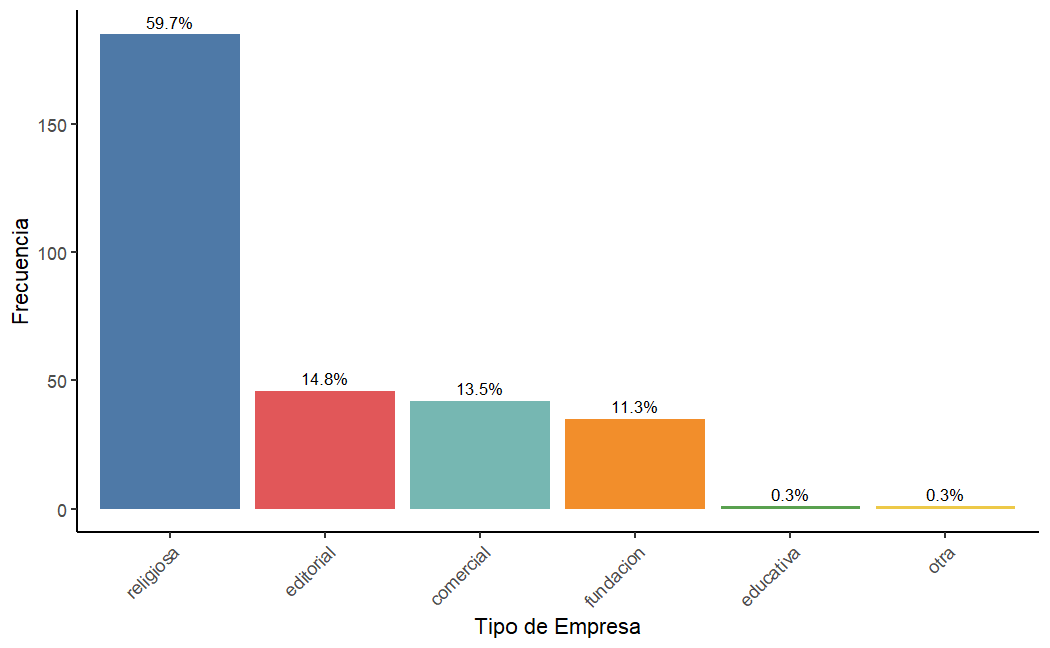
\includegraphics[width=0.8\textwidth]{figuras/Tipo_Empresa.png}
    \caption{\label{figempresa}Distribución del volumen transaccional por tipo de empresa.}
    \end{figure}
    
    \begin{figure}[H]
    \centering
    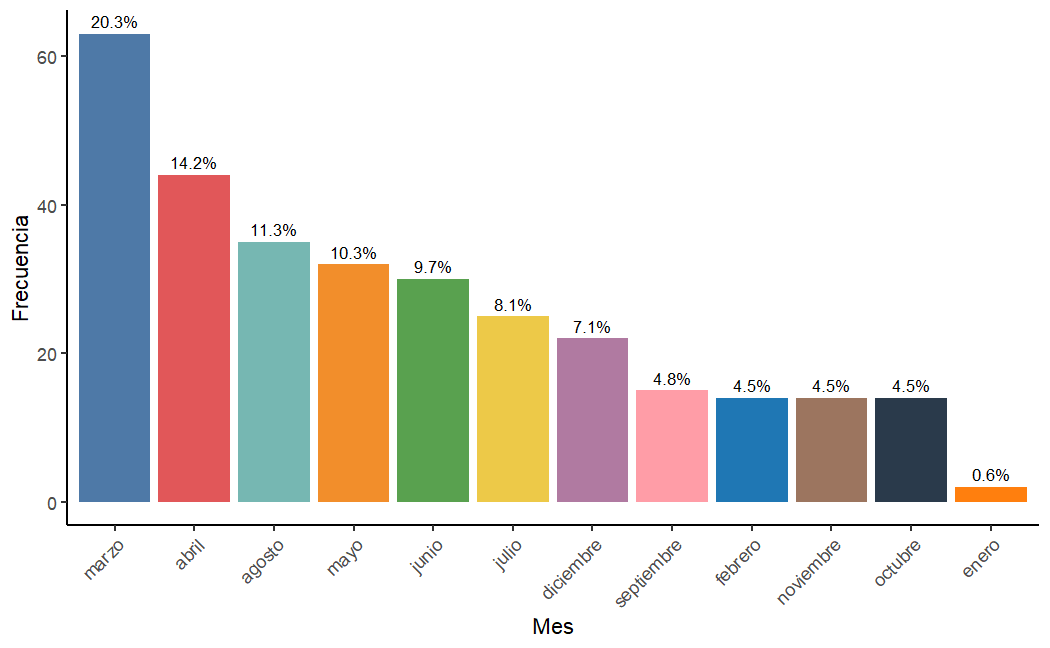
\includegraphics[width=0.8\textwidth]{figuras/Mes.png}
    \caption{\label{figmes}Distribución del volumen transaccional por mes.}
    \end{figure}
    
    En la Figura~\ref{figorigen} se observa que el 94\% del volumen de ventas proviene del mercado nacional. Aunque el segmento internacional es reducido, su identificación resulta relevante para caracterizar perfiles potencialmente diferenciados de asignación del gasto.

    La Figura~\ref{figciudad} muestra una fuerte concentración geográfica del volumen transaccional, con Bogotá como principal centro de demanda. Casos como Frontino, con una participación relevante pese a su menor tamaño relativo, sugieren la presencia de clientes institucionales de alto volumen.
    
    \begin{figure}[H]
    \centering
    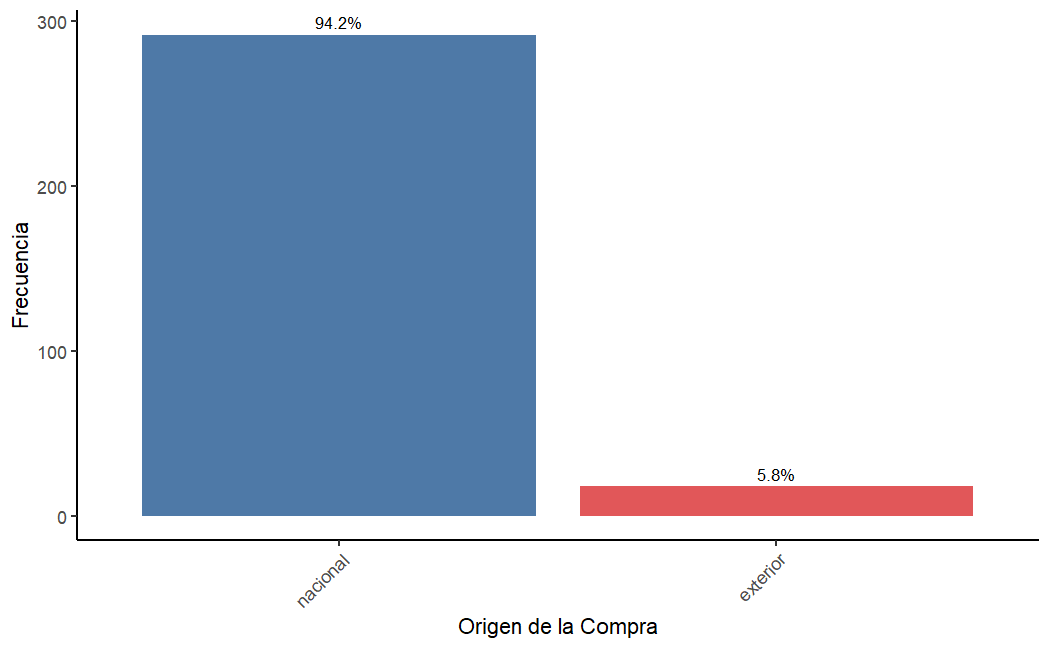
\includegraphics[width=0.8\textwidth]{figuras/Origen de Compra.png}
    \caption{\label{figorigen}Distribución del volumen transaccional según el origen de la compra.}
    \end{figure}
    
    \begin{figure}[H]
    \centering
    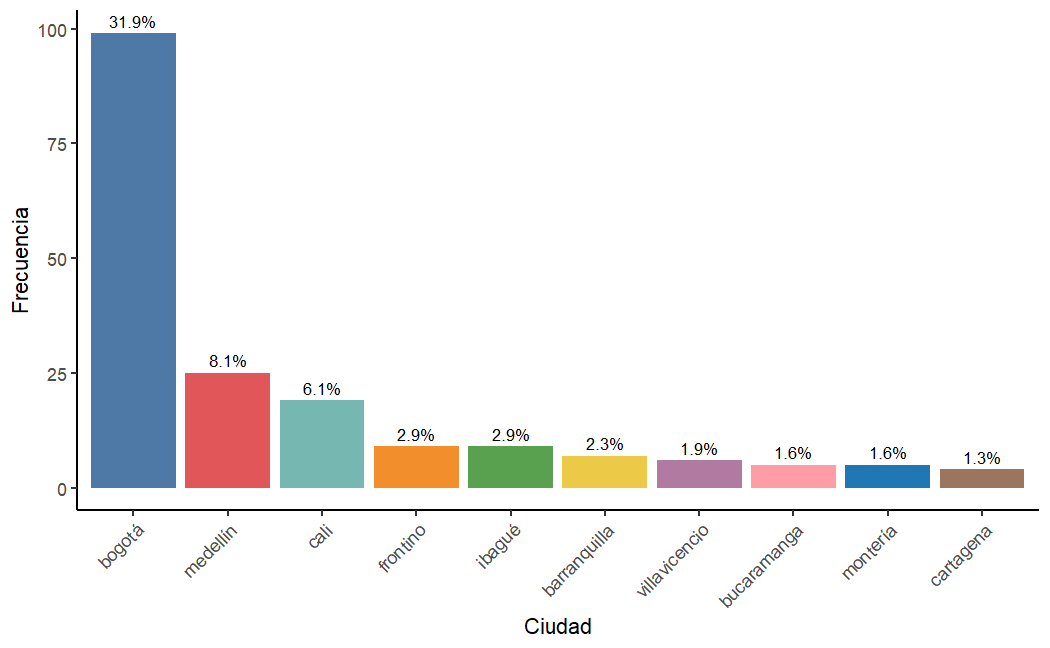
\includegraphics[width=0.8\textwidth]{figuras/Ciudad.png}
    \caption{\label{figciudad}Distribución del volumen transaccional por ciudad (Top 10).}
    \end{figure}
    
    En cuanto al portafolio de productos, la Figura~\ref{figtipoproducto} indica que cerca del 90\% del volumen corresponde a biblias, lo que implica una alta concentración en un único tipo de producto. En consecuencia, la diferenciación entre clientes se explica principalmente por variables de volumen, frecuencia, formato y diversidad de referencias, más que por la elección entre categorías.

    Finalmente, la Figura~\ref{figtamano} muestra una marcada preferencia por el formato Biblia Taco 60, que concentra cerca del 70\% del volumen total, lo que sugiere una estandarización importante en las decisiones de compra.

     El análisis exploratorio documenta la existencia de heterogeneidad estructural entre clientes, concentración del volumen transaccional y escalas altamente dispares entre covariables. Estos resultados se interpretan exclusivamente desde una perspectiva descriptiva y constituyen el insumo empírico para el diseño del preprocesamiento posterior, donde se implementan criterios formales para el tratamiento de valores extremos, la estandarización y el control de redundancias entre covariables.
    
    \begin{figure}[H]
    \centering
    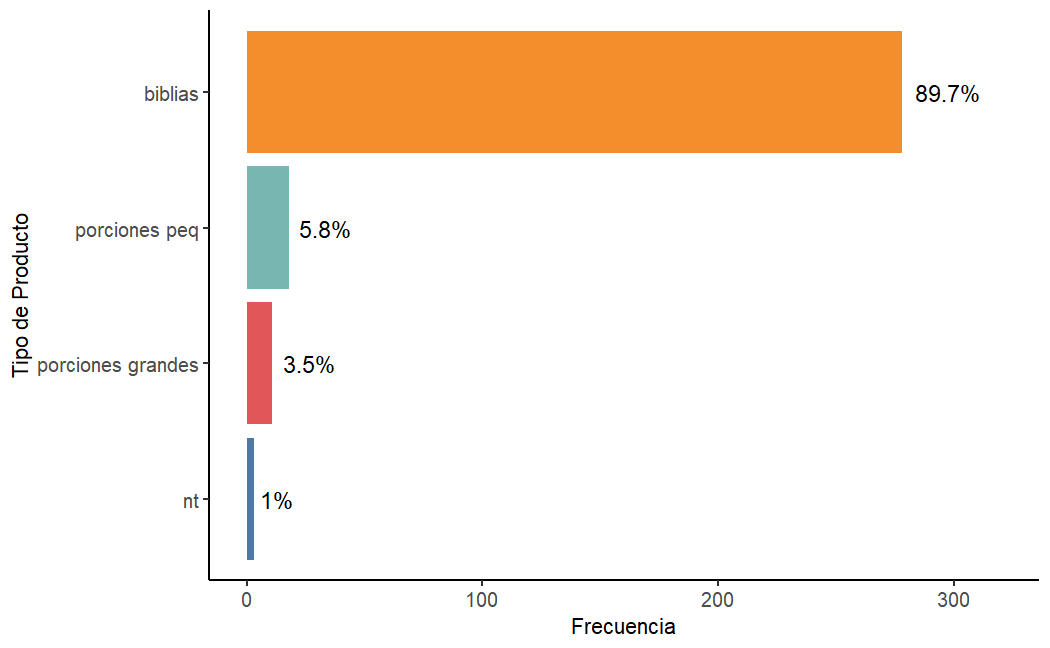
\includegraphics[width=0.8\textwidth]{figuras/Tipo Producto.png}
    \caption{\label{figtipoproducto}Distribución del volumen transaccional por tipo de producto.}
    \end{figure}
    
    \begin{figure}[H]
    \centering
    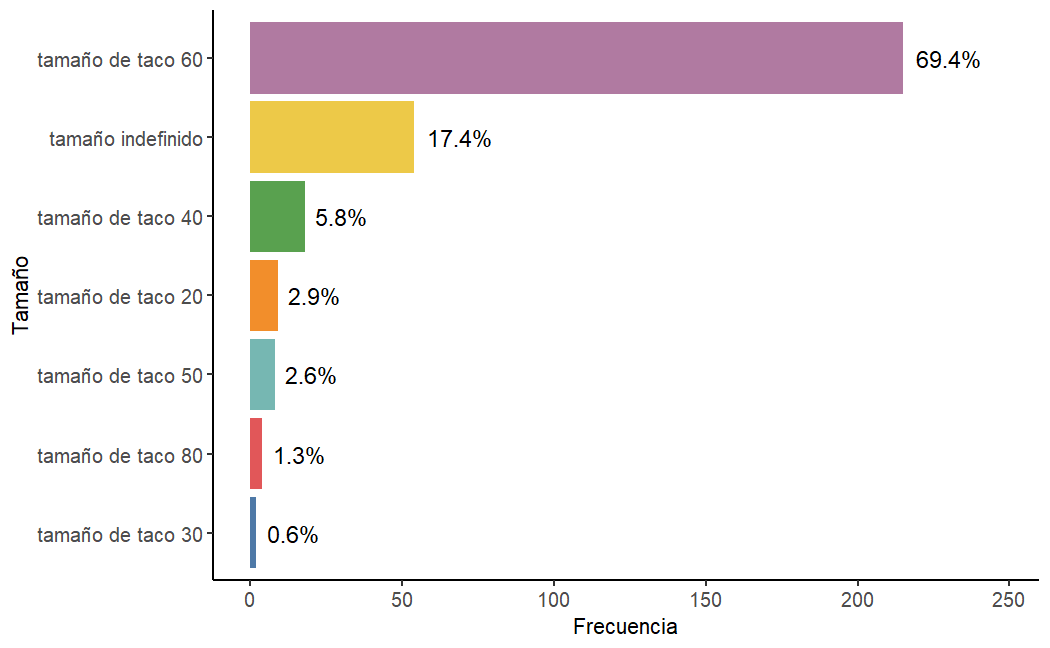
\includegraphics[width=0.8\textwidth]{figuras/Tamaño.png}
    \caption{\label{figtamano}Distribución del volumen transaccional por tamaño de producto.}
    \end{figure}
    
%--------------------------------------------------
\section{Preprocesamiento}

\subsubsection{Análisis de asociación entre variables cuantitativas}
        Con el fin de evaluar el grado de asociación entre las variables cuantitativas predictoras y detectar posibles redundancias, se calculó el coeficiente de correlación de Spearman. 
        
        La Tabla~\ref{tab:corr_cuantitativas} presenta las correlaciones de Spearman más altas observadas entre pares de variables cuantitativas. Con fines de depuración, se consideraron únicamente aquellas asociaciones cuyo coeficiente fue mayor o igual a 0.70 en valor absoluto, umbral comúnmente utilizado para identificar relaciones fuertes y potencialmente redundantes.

         De manera complementaria, se observa que la variable \textit{recency\_days} presenta correlaciones negativas moderadas a altas con el resto de variables cuantitativas (en el rango aproximado de -0.50 a -0.70), lo cual indica que mayores tiempos desde la última compra se asocian sistemáticamente con menores niveles de frecuencia, gasto y volumen adquirido. Dado que estas correlaciones negativas no superan el umbral absoluto adoptado para la identificación de asociaciones fuertes, no se incluyen en la tabla; no obstante, su patrón resulta plenamente consistente con la lógica del marco RFM.

        El análisis revela una fuerte asociación entre las variables \textit{Monetary}, \textit{Costo Total} y \textit{Utilidad Bruta}, con coeficientes de Spearman superiores a 0.95. Dado que estas variables capturan esencialmente la misma dimensión de escala económica del cliente, se decide conservar únicamente \textit{Monetary}, por su interpretación directa y su uso estándar en análisis RFM, y eliminar las restantes para reducir redundancia en el diseño del modelo.
        
        \begin{table}[H]
        \centering
        \caption{Correlaciones de Spearman más altas entre variables cuantitativas}
        \label{tab:corr_cuantitativas}
        \renewcommand{\arraystretch}{1.2}
        \resizebox{\textwidth}{!}{%
        \begin{tabular}{l l c @{~~~~} l l c}
        \hline
        \textbf{Variable 1} & \textbf{Variable 2} & \textbf{Spearman} &
        \textbf{Variable 1} & \textbf{Variable 2} & \textbf{Spearman} \\
        \hline
        Costo total & Monetary & 0.99 &
        Cantidad & Utilidad bruta & 0.85 \\
        
        Monetary & Utilidad bruta & 0.98 &
        Valor Bruto & Valor neto & 0.82 \\
        
        Costo total & Utilidad bruta & 0.96 &
        Utilidad bruta & Valor bruto & 0.79 \\
        
        Frequency & Skus distintos & 0.94 &
        Costo total & Frequency & 0.79 \\
        
        Frequency & Valor bruto & 0.93 &
        Monetary & Valor bruto & 0.78 \\
        
        Cantidad & Costo total & 0.90 &
        Frequency & Monetary & 0.78 \\
        
        Cantidad & Monetary & 0.89 &
        Costo total & Valor bruto & 0.78 \\
        
        Skus distintos & Valor bruto & 0.87 &
        Frequency & Utilidad bruta & 0.77 \\
        
        Descuentos & Valor neto & 0.76 &
        Frequency & Valor neto & 0.74 \\
        
        Costo total & Skus distintos & 0.71 &
        Cantidad & Frequency & 0.70 \\
        \hline
        \end{tabular}%
        }
        \end{table}

        Asimismo, se identifican correlaciones elevadas entre \textit{Frequency}, \textit{Skus Distintos} y \textit{Valor Bruto}. En este caso, se optó por conservar \textit{Frequency}, dado que representa de manera más directa la recurrencia del comportamiento de compra, y eliminar las otras variables altamente correlacionadas.
        
        Finalmente, dado que \textit{Valor Neto} presenta asociaciones fuertes con múltiples variables monetarias y de frecuencia, se decidió excluirla del conjunto de covariables para evitar solapamientos informativos.
        
        Como resultado de este proceso de depuración, se obtuvo el conjunto final de variables cuantitativas que se utilizarán en la construcción de la matriz de diseño del modelo \emph{pogit}, el cual se resume en la Tabla~\ref{tab:depuracion_cuantitativas}.
        
        \begin{table}[H]
        \centering
        \caption{Variables cuantitativas seleccionadas y eliminadas tras el análisis de asociación}
        \label{tab:depuracion_cuantitativas}
        \renewcommand{\arraystretch}{1.2}
        \begin{tabular}{p{7cm} p{7cm}}
        \hline
        \textbf{Permanecen en el modelo} & \textbf{Eliminadas del modelo} \\
        \hline
        \textit{monetary}, \textit{frequency} 
        & \textit{costo\_total}, \textit{utilidad\_bruta} \\
        \textit{recency\_days}, \textit{descuentos} 
        & \textit{valor\_bruto}, \textit{skus\_distintos} \\
        \textit{cantidad} 
        & \textit{valor\_neto} \\
        \hline
        \end{tabular}
        \end{table}

%--------------------------------------------------
\subsubsection{Correlación de Cramér}
        Con el fin de evaluar la asociación y posible redundancia entre las variables cualitativas, se empleó el estadístico V de Cramér, el cual es apropiado para medir la intensidad de asociación entre variables categóricas nominales y ordinales. A diferencia de medidas como la correlación de Spearman, los valores de Cramér tienden a ser más bajos incluso en presencia de relaciones estructuralmente fuertes; por esta razón, en la literatura se considera que asociaciones relevantes pueden observarse desde valores cercanos a 0.4.  
        
        En este estudio se adoptó un umbral conservador de 0.5 para identificar asociaciones fuertes entre variables cualitativas, con el objetivo de detectar redundancias sustantivas que pudieran generar colinealidad, sobreparametrización e inestabilidad en la estimación del modelo \emph{pogit}. Este análisis se utiliza exclusivamente como un criterio de depuración y selección de covariables, y no como un mecanismo de inferencia causal.
        
        La Tabla~\ref{tab:corr_cualitativas} presenta los pares de variables cualitativas con los valores más altos del estadístico V de Cramér, ordenados de mayor a menor asociación.

        Los resultados evidencian patrones claros de redundancia estructural entre varias capas de información categórica. En particular, la variable \textit{Tipo} presenta asociaciones extremadamente altas con \textit{Tipo Factura}, \textit{Audiencia} y \textit{País}, con valores de Cramér superiores a 0.95. Dado que \textit{Tipo} captura de manera sintética patrones relevantes del comportamiento del cliente y resume información contenida en dichas variables, se opta por conservarla y excluir las variables altamente redundantes asociadas.

        De manera similar, \textit{Departamento} muestra asociaciones elevadas con \textit{País}, \textit{Ciudad} y \textit{Zona}. Desde una perspectiva de modelamiento, \textit{Departamento} representa un nivel geográfico intermedio que permite capturar heterogeneidad territorial sin incurrir en la alta cardinalidad de \textit{Ciudad} ni en la excesiva agregación de \textit{País}. En consecuencia, se conserva \textit{Departamento} y se excluyen las demás variables geográficas redundantes.
        
        En relación con la estructura del producto, se observan asociaciones fuertes entre \textit{Clase 2}, \textit{Grupo}, \textit{Nombre de Clase} y \textit{SKU}, lo que indica una jerarquía altamente colineal. Para evitar sobreparametrización, se conserva la variable \textit{Categoría}, la cual se ubica en un nivel intermedio de la jerarquía del producto y permite capturar diferencias relevantes sin introducir redundancia excesiva. Adicionalmente, se mantiene la variable \textit{Tamaño}, dado que aporta información complementaria no completamente contenida en las demás variables del producto.
        
        \begin{table}[H]
        \centering
        \caption{Correlaciones de Cramér más altas entre variables cualitativas}
        \label{tab:corr_cualitativas}
        \renewcommand{\arraystretch}{1.15}
        \resizebox{\textwidth}{!}{%
        \begin{tabular}{l l c @{\hspace{1cm}} l l c}
        \hline
        \textbf{Variable 1} & \textbf{Variable 2} & \textbf{Cramér} &
        \textbf{Variable 1} & \textbf{Variable 2} & \textbf{Cramér} \\
        \hline
        Tipo & Tipo Factura & 0.99 &
        Clase 2 & Nombre de Clase & 0.83 \\
        
        País & Tipo & 0.97 &
        Categoría & SKU & 0.76 \\
        
        Audiencia & Tipo & 0.96 &
        Grupo & SKU & 0.75 \\
        
        Departamento & País & 0.95 &
        Clase 2 & SKU & 0.73 \\
        
        Tipo & Zona & 0.93 &
        SKU & Tipo Factura & 0.70 \\
        
        Nombre de Clase & Tamaño & 0.93 &
        Nombre de Clase & SKU & 0.66 \\
        
        Departamento & Tipo & 0.93 &
        SKU & Tamaño & 0.65 \\
        
        Ciudad & Departamento & 0.90 &
        Departamento & Zona & 0.62 \\
        
        Ciudad & País & 0.86 &
        Audiencia & Tipo Factura & 0.62 \\
        
        Ciudad & Tipo & 0.84 &
        Clase 2 & Tamaño & 0.61 \\
        \hline
        \end{tabular}%
        }
        \end{table}

        Mantener simultáneamente variables altamente asociadas habría incrementado la colinealidad entre regresores categóricos y comprometido la estabilidad numérica y la interpretabilidad de los coeficientes del modelo \emph{pogit}. En consecuencia, la selección final de variables cualitativas responde a un equilibrio entre capacidad explicativa, parsimonia y coherencia económica.
        
        La Tabla~\ref{tab:vars_cualitativas_finales} resume las variables cualitativas finalmente seleccionadas para su inclusión en el modelo.
        
        \begin{table}[H]
        \centering
        \caption{Variables cualitativas seleccionadas para el modelo}
        \label{tab:vars_cualitativas_finales}
        \begin{tabular}{p{14cm}}
        \hline
        \textbf{Variables incluidas en el modelo} \\
        \hline
        Tipo, Departamento, Categoría, Tamaño, Mes, Tipo de Empresa, Condición \\
        \hline
        \end{tabular}
        \end{table}
        
\subsection{Estandarización de variables}

    Las variables cuantitativas se estandarizaron previamente a la implementación de los algoritmos de reducción de dimensionalidad (PCA), segmentación (k-means y k-medoids) y del modelo \emph{pogit}. Este paso es necesario para garantizar que todas las variables contribuyan de manera comparable en procedimientos sensibles a la escala, evitando que aquellas con mayor magnitud dominen indebidamente los resultados.
    
    La estandarización se realizó exclusivamente utilizando información observada en la ventana de características \(T_1\), siguiendo la formulación descrita en la metodología. Este procedimiento transforma cada variable cuantitativa a una escala con media cero y desviación estándar unitaria, sin alterar las relaciones ordinales entre observaciones ni introducir información futura.

\begin{table}[H]
    \centering
    \caption{Valores estandarizados de variables cuantitativas para seis clientes seleccionados, calculados a partir de la ventana de características \(T_1\).}
    \label{tab:tablaestandarizada}
    \small
    \renewcommand{\arraystretch}{1.2}
    \begin{tabular}{lrrrrrr}
    \hline
    \textbf{Variable} & \textbf{Obs 1} & \textbf{Obs 2} & \textbf{Obs 3} & \textbf{Obs 4} & \textbf{Obs 5} & \textbf{Obs 6} \\
    \hline
    Recency      & -0.53 & -0.15 & -0.88 & -0.84 & -0.44 &  1.02 \\
    Frequency          &  0.21 & -0.12 &  0.62 &  0.34 & -0.21 & -0.16 \\
    Monetary           &  2.23 &  0.60 &  1.51 &  0.81 &  2.23 &  1.37 \\
    Valor bruto       & -0.11 & -0.20 &  0.03 & -0.01 & -0.28 & -0.22 \\
    Skus distintos    &  1.29 &  0.07 &  2.07 &  1.25 & -0.22 & -0.20 \\
    descuento               & -1.50 & -1.50 & -1.50 & -1.50 & -1.50 & -1.50 \\
    Valor neto        & -0.29 & -0.29 & -0.29 & -0.29 & -0.29 & -0.29 \\
    Cantidad               &  5.14 &  2.17 &  5.87 &  1.14 &  3.24 &  0.67 \\
    Costo total        &  2.61 &  0.74 &  1.54 &  0.93 &  2.61 &  1.38 \\
    Utilidad bruta    &  1.41 &  0.31 &  1.35 &  0.53 &  1.40 &  1.25 \\
    \hline
    \end{tabular}
    \end{table}
    
    La Tabla~\ref{tab:tablaestandarizada} presenta, a modo ilustrativo, los valores estandarizados de un subconjunto de variables cuantitativas para los primeros seis clientes. Estos registros se muestran únicamente con fines demostrativos del proceso de transformación, y no se utilizan para inferencia directa. Cabe señalar que la tabla presentada tiene un carácter exclusivamente ilustrativo y muestra el efecto de la transformación de estandarización sobre un subconjunto amplio de variables cuantitativas originalmente construidas. Algunas de estas variables son posteriormente excluidas del modelo final como resultado del análisis de asociación y depuración descrito en las subsecciones previas. En consecuencia, los valores mostrados no se utilizan para inferencia directa y no representan necesariamente el conjunto final de covariables empleadas en la estimación del modelo \emph{pogit}.

    
%--------------------------------------------------
\section{Construcción de matrices de diseño del modelo \emph{pogit}}

    Las configuraciones presentadas en la Tabla~\ref{tab:pogit_design_matrices} no representan modelos conceptualmente distintos, sino distintas parametrizaciones del mismo marco \emph{pogit}. Estas parametrizaciones se diseñan con el objetivo de evaluar la estabilidad estructural de las inferencias sobre la participación en la billetera (SoW) y el tamaño de la billetera (SioW) frente a variaciones en la selección de covariables y en el grado de parsimonia de las matrices de diseño.

    \begin{table}[H]
    \centering
    \caption{Configuraciones de matrices de diseño utilizadas en la implementación del modelo \emph{pogit}. Cada versión corresponde a una especificación alternativa de las matrices $\mathbf{W}$ (componente SoW) y $\mathbf{V}$ (componente SioW).}
    \label{tab:pogit_design_matrices}
    \renewcommand{\arraystretch}{1.2}
    \resizebox{\textwidth}{!}{%
    \begin{tabular}{c p{5.2cm} p{6.5cm}}
    \hline
    \textbf{Versión} & \textbf{Matriz $\mathbf{W}$ (SoW)} & \textbf{Matriz $\mathbf{V}$ (SioW)} \\
    \hline
    1 & RFM completos + condiciones del cliente &
    Ubicación geográfica + categoría de producto + mes + tipo de empresa \\
    2 & RFM completos &
    Ubicación geográfica + tipo de empresa \\
    3 & RFM completos &
    Categoría de producto + tipo de cliente / empresa \\
    4 & RFM completos &
    Categoría de producto + mes del año \\
    5 & RFM completos &
    Categoría de producto \\
    6 & RFM completos &
    Indicadores mensuales \\
    7 & PC1 y PC2 (PCA) + condiciones del cliente &
    Ubicación geográfica + tipo de empresa \\
    8 & PC1 y PC2 (PCA) + condiciones del cliente &
    Ubicación geográfica + tipo de empresa + categoría de producto \\
    9 & PC1 y PC2 (PCA) &
    Tipo de empresa \\
    \hline
    \end{tabular}}
    \end{table}
    
    Todas las configuraciones se construyen a partir del mismo conjunto de datos preprocesados y estandarizados, descrito en las secciones metodológicas previas. En consecuencia, las diferencias entre versiones no obedecen a transformaciones adicionales de los datos, sino exclusivamente a cambios en la composición de las matrices $\mathbf{W}$ y $\mathbf{V}$, manteniendo fija la estructura del modelo \emph{pogit} y el procedimiento de estimación.
    
    Las versiones consideradas se organizan siguiendo un criterio incremental de parsimonia, que afecta tanto a la representación del comportamiento transaccional en la matriz $\mathbf{W}$ como a la caracterización de la heterogeneidad estructural en la matriz $\mathbf{V}$. En este esquema, se parte de especificaciones basadas en variables transaccionales originales y se avanza progresivamente hacia representaciones más sintéticas mediante selección de covariables o reducción de dimensionalidad.
    
    Las versiones 1 a 6 corresponden a especificaciones en las que la matriz $\mathbf{W}$ se construye a partir de variables transaccionales originales del tipo RFM. En estas versiones, la composición de la matriz $\mathbf{V}$ se modifica de manera controlada con el fin de evaluar la sensibilidad del componente de intensidad (SioW) a distintas fuentes de heterogeneidad estructural, tales como la localización geográfica, la categoría de producto, la estacionalidad o el tipo de empresa.
    
    Las versiones 7 a 9 introducen una representación alternativa de la matriz $\mathbf{W}$ basada en componentes principales obtenidas mediante PCA aplicado a las variables transaccionales cuantitativas. En estas especificaciones, las componentes principales reemplazan a las variables RFM originales como insumo del componente SoW, permitiendo evaluar la robustez de las inferencias del modelo frente a una síntesis ortogonal y parsimoniosa de la información transaccional. Las condiciones del cliente se mantienen en $\mathbf{W}$ únicamente cuando representan modalidades operativas directamente asociadas al comportamiento transaccional, en coherencia con la definición metodológica previa.
    
    Las matrices de diseño definidas en esta sección constituyen el insumo estructural del modelo \emph{pogit} y permanecen fijas durante la estimación. Las técnicas de reducción de dimensionalidad y segmentación introducidas en la sección siguiente no intervienen en el proceso de estimación del modelo, sino que se utilizan con fines exploratorios, interpretativos y de evaluación estructural de las estimaciones obtenidas.
    
%--------------------------------------------------
\section{Reducción de dimensionalidad y segmentación ex-
ploratoria} 

\subsection{Análisis de PCA para la reducción de dimensionalidad}
        La Figura~\ref{figScree} presenta el gráfico de sedimentación correspondiente al Análisis de Componentes Principales (PCA), estimado exclusivamente sobre el conjunto de entrenamiento y construido a partir de las variables cuantitativas observadas en la ventana de características \(T_1\). Este gráfico permite evaluar empíricamente la proporción de varianza explicada por cada componente y constituye el principal criterio para determinar la dimensionalidad efectiva del espacio reducido.

        Cabe enfatizar que el PCA se aplica sobre el conjunto completo de variables transaccionales cuantitativas
        previamente estandarizadas, sin requerir una depuración previa por correlación. A diferencia del modelo \emph{pogit}, donde la parsimonia y la interpretabilidad de los coeficientes son criterios centrales, el PCA se beneficia explícitamente de la presencia de variables correlacionadas.

        De acuerdo con la Figura~\ref{figScree}, el primer componente principal (PC1) explica el 52.1\% de la varianza total, mientras que el segundo componente (PC2) explica un 25.8\% adicional. En conjunto, las dos primeras componentes concentran aproximadamente el 78.0\% de la variabilidad total del conjunto de variables cuantitativas. A partir del tercer componente, la varianza explicada individual desciende por debajo del 11\%, y los componentes subsiguientes aportan contribuciones marginales decrecientes. La presencia de un punto de inflexión claramente identificable tras el segundo componente respalda empíricamente la decisión de centrar el análisis en las dos primeras dimensiones principales, dado que la incorporación de componentes adicionales aporta información incremental limitada.
        
        \begin{figure}[H]
        \centering
        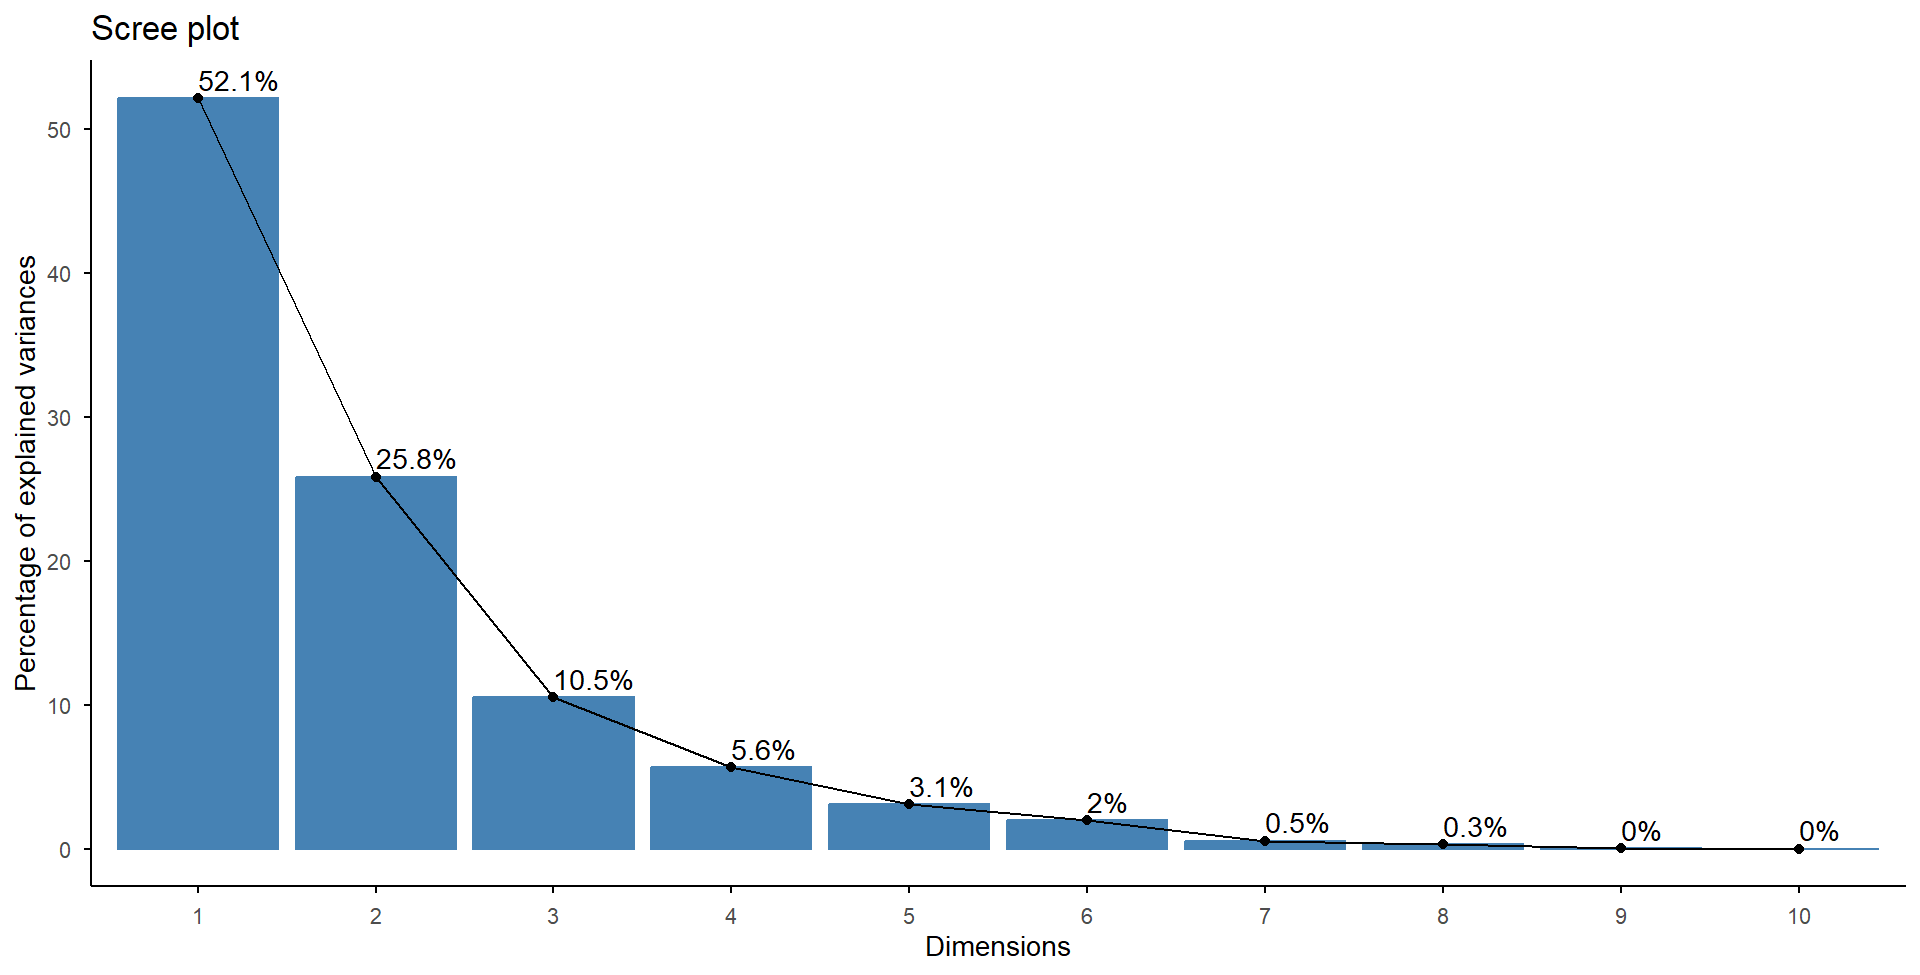
\includegraphics[width=0.8\textwidth]{figuras/Sedimentación.png}
        \caption{\label{figScree}Gráfico de sedimentación.}
        \end{figure}
        
        La Figura~\ref{figContriDim1} muestra la contribución relativa de cada variable original a la primera componente principal (PC1). Se observa que las variables \textit{Frequency}, \textit{Utilidad bruta}, \textit{Valor bruto}, \textit{SKUs distintos}, \textit{Monetary} y \textit{Valor neto} presentan contribuciones individuales superiores al umbral del 10\%, lo que indica que estas variables son las principales responsables de la variabilidad capturada por esta dimensión.

        El patrón de contribuciones observado en la Figura~\ref{figContriDim1} permite interpretar PC1 como un eje asociado al \emph{comportamiento económico agregado del cliente}. Esta componente sintetiza de manera conjunta la recurrencia de compra (\textit{Frequency}), la magnitud del gasto (\textit{Monetary}), el volumen económico generado (\textit{Valor bruto} y \textit{Valor neto}), la rentabilidad (\textit{Utilidad bruta}) y la amplitud del portafolio adquirido (\textit{SKUs distintos}). En consecuencia, valores elevados de PC1 corresponden a clientes con relaciones comerciales intensivas y de alto valor económico, mientras que valores bajos reflejan perfiles con baja intensidad transaccional.

        La Figura~\ref{figContriDim2} presenta las contribuciones de las variables a la segunda componente principal (PC2). En este caso, las variables con contribuciones superiores al 10\% son \textit{Costo total}, \textit{Descuentos}, \textit{Monetary}, \textit{Cantidad} y \textit{Valor neto}.

        A diferencia de PC1, la segunda componente captura una dimensión asociada a la \emph{estructura del gasto y su relación con costos y descuentos}. En particular, PC2 discrimina entre clientes que, aun presentando niveles similares de gasto monetario, difieren en la cantidad adquirida, en los costos asociados a sus compras y en la intensidad del uso de descuentos. Puntuaciones elevadas en esta dimensión reflejan perfiles con mayor volumen físico, mayores costos y una mayor incidencia de descuentos, mientras que puntuaciones bajas corresponden a estructuras de compra más simples o menos dependientes de incentivos comerciales.
        
        \begin{figure}[H]
        \centering
        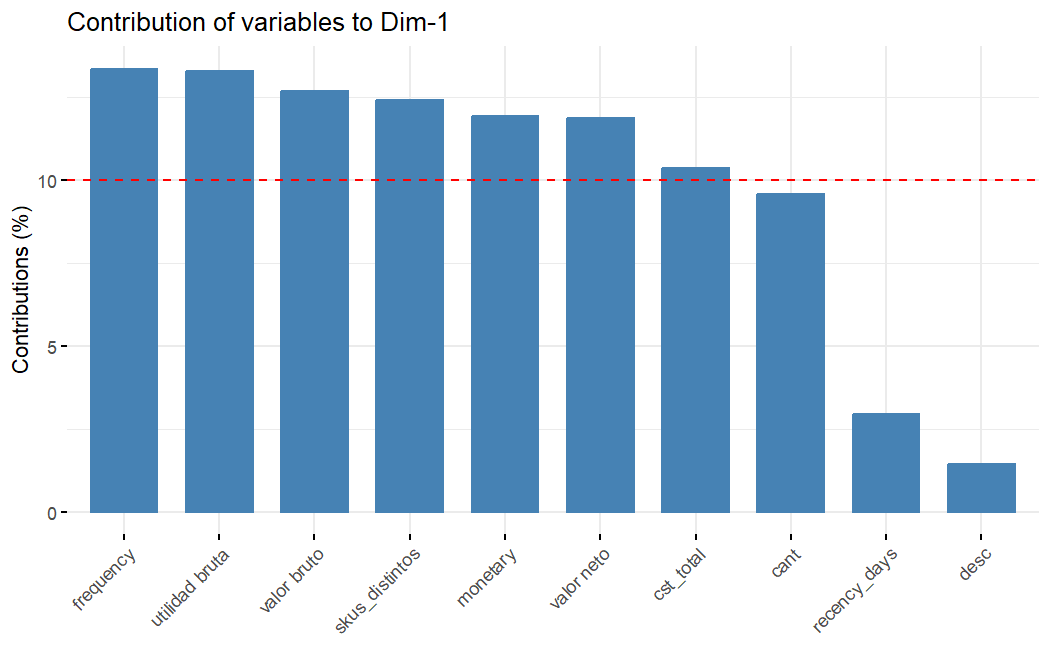
\includegraphics[width=0.8\textwidth]{figuras/Contri_Dim1.png}
        \caption{\label{figContriDim1}Contribución de las variables a la componente PC1.}
        \end{figure}
        
        \begin{figure}[H]
        \centering
        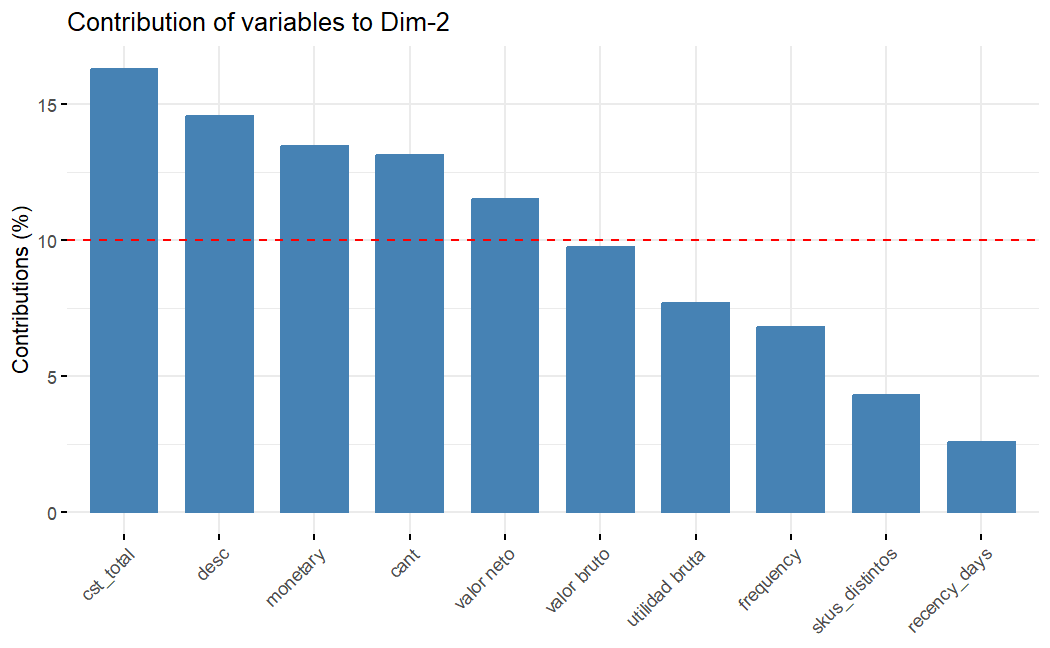
\includegraphics[width=0.8\textwidth]{figuras/Contri_Dim2.png}
        \caption{\label{figContriDim2}Contribución de las variables a la componente PC2.}
        \end{figure}
        
        La interpretación conjunta de ambas componentes se refuerza mediante el análisis del círculo de correlación presentado en la Figura~\ref{figPCAvars}, donde se visualizan simultáneamente la dirección y la magnitud de las cargas de cada variable en el plano definido por PC1 y PC2.
        
        \begin{figure}[H]
        \centering
        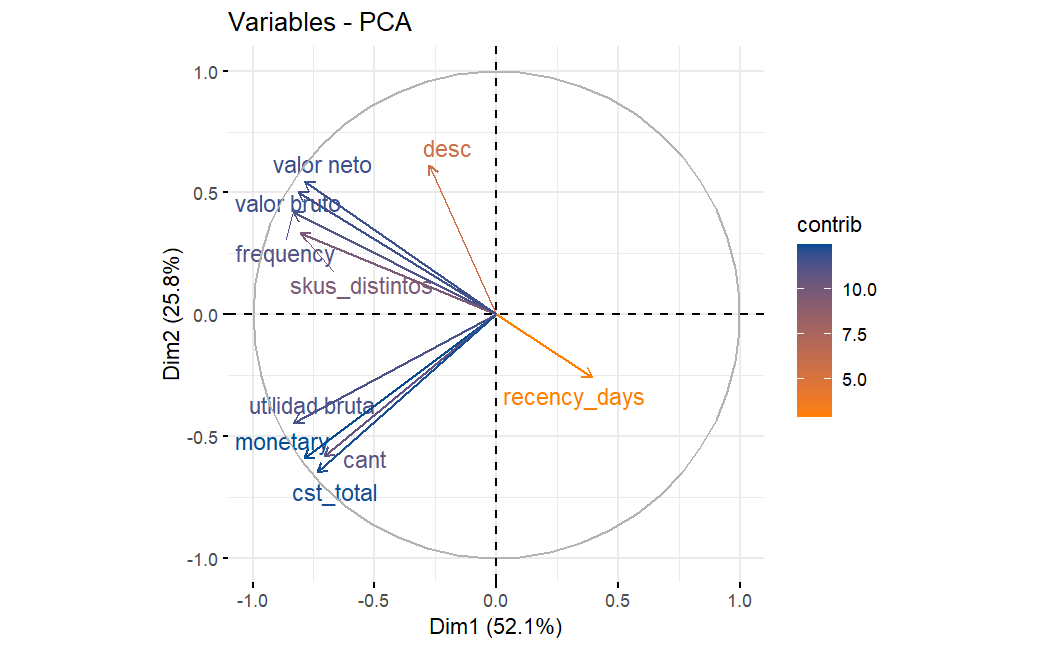
\includegraphics[width=0.8\textwidth]{figuras/Variables PCA.png}
        \caption{\label{figPCAvars}Círculo de correlación de las variables en el plano PC1--PC2.}
        \end{figure}
        
        En la Figura~\ref{figPCAvars} se observa que las variables \textit{Costo total}, \textit{Monetary}, \textit{Cantidad} y \textit{Utilidad bruta} apuntan en direcciones muy similares, lo que confirma una alta correlación estructural entre ellas y respalda empíricamente los resultados del análisis de correlación bivariada. Esta superposición justifica la conservación de una única variable representativa de esta dimensión económica, en particular \textit{Monetary}, dada su interpretación directa y su rol central dentro del esquema RFM.
        
        De manera análoga, las variables \textit{Valor bruto}, \textit{Valor neto} y \textit{Frequency} presentan una alineación estrecha, lo que indica que capturan información parcialmente redundante asociada al tamaño y recurrencia de la relación comercial. En este contexto, la retención de \textit{Frequency} permite preservar una medida directa de recurrencia conductual, mientras que \textit{Valor neto} aporta información complementaria sobre el monto efectivamente pagado tras la aplicación de descuentos.
        
        Finalmente, las variables \textit{Descuentos} y \textit{Recency} aparecen relativamente aisladas en el espacio factorial, con ángulos amplios respecto al resto de variables. Este patrón indica que aportan información adicional no redundante, asociada respectivamente a la política comercial aplicada al cliente y al tiempo transcurrido desde la última compra. En consecuencia, su inclusión resulta relevante para capturar dimensiones del comportamiento del cliente que no están explicadas exclusivamente por el volumen económico.
        
        Los resultados del PCA confirman la existencia de una estructura latente de baja dimensionalidad dominada por dos ejes principales: (i) una dimensión asociada a la intensidad y valor económico global del cliente (PC1) y (ii) una dimensión vinculada a la estructura del gasto, los costos y la sensibilidad a descuentos (PC2). Estas conclusiones son coherentes con los resultados del análisis de asociación previo y respaldan empíricamente las decisiones de selección y depuración de variables adoptadas antes del modelamiento del \emph{pogit}.

\subsection{Análisis de conglomerados mediante K-means}
        Con el objetivo de identificar segmentos homogéneos de clientes a partir de su comportamiento transaccional, se aplicó el algoritmo de agrupación
        \emph{K-means} sobre el conjunto de entrenamiento, utilizando exclusivamente las variables cuantitativas previamente seleccionadas: \textit{Monetary},
        \textit{Frequency}, \textit{Recency}, \textit{Descuentos} y \textit{Cantidad}.
        Todas las variables fueron transformadas y estandarizadas según lo descrito en la sección metodológica, garantizando comparabilidad en escala y evitando la dominancia de variables con mayor magnitud.
        
        La selección del número óptimo de clústeres \(k\) se realizó mediante el uso complementario del Método del Codo y del índice de Silhouette, con el fin de balancear compactación interna, separación entre grupos y parsimonia del modelo de segmentación.
        
        La Figura~\ref{figElbow} muestra la evolución de la suma de errores cuadráticos intra--clúster (WSS) en función de \(k\). Se observa una reducción pronunciada del WSS al pasar de \(k = 1\) a \(k = 3\), seguida de una disminución progresivamente más suave a partir de ese punto. Este cambio claro de pendiente identifica un “codo” alrededor de \(k = 3\), lo que sugiere que incrementos adicionales en el número de clústeres generan mejoras marginales en la compactación interna.
        
        De forma complementaria, la Figura~\ref{figSilhouette} presenta el valor promedio del índice de Silhouette para distintos valores de \(k\). El índice alcanza sus valores máximos para \(k = 2\), \(k = 3\) y \(k = 4\), con valores comprendidos entre 0.460 y 0.470, lo que indica una cohesión interna adecuada y una separación razonable entre grupos. A partir de \(k = 5\), el índice desciende de manera marcada hasta valores cercanos a 0.320, evidenciando una pérdida sustancial de calidad en la partición.

         Considerando conjuntamente ambos criterios, se seleccionó \(k = 4\) como una solución de compromiso entre parsimonia, calidad del agrupamiento y capacidad interpretativa de los segmentos resultantes. Esta elección permite capturar heterogeneidad relevante en el comportamiento de los clientes sin incurrir en sobresegmentación.

        \begin{figure}[H]
        \centering
        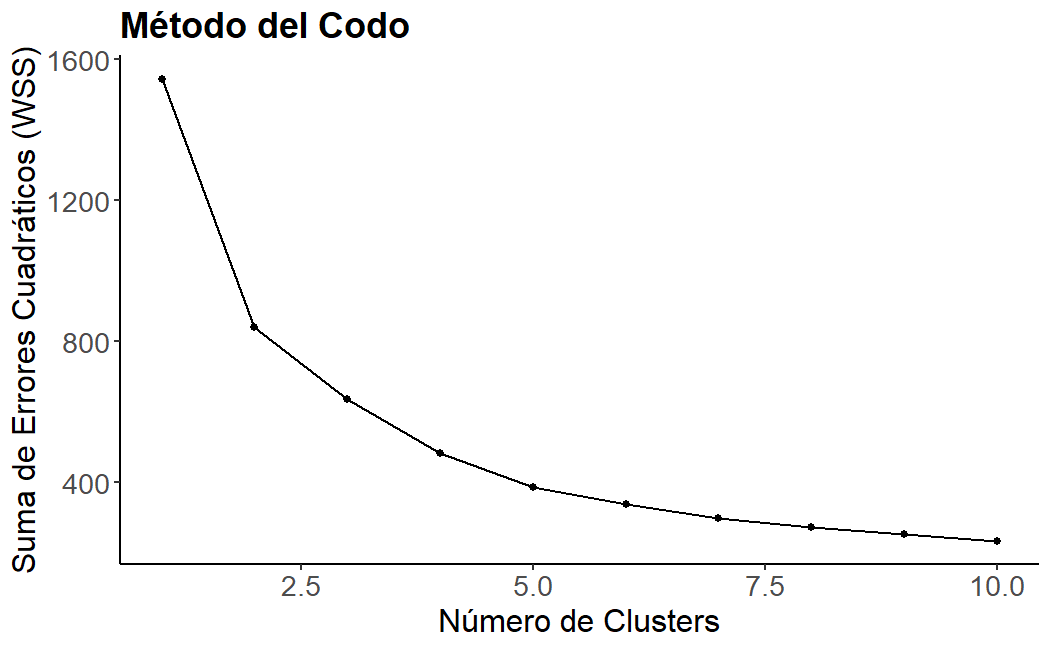
\includegraphics[width=0.8\textwidth]{figuras/Método del Codo.png}
        \caption{\label{figElbow}Método del Codo para la selección del número de clústeres.}
        \end{figure}
        
        \begin{figure}[H]
        \centering
        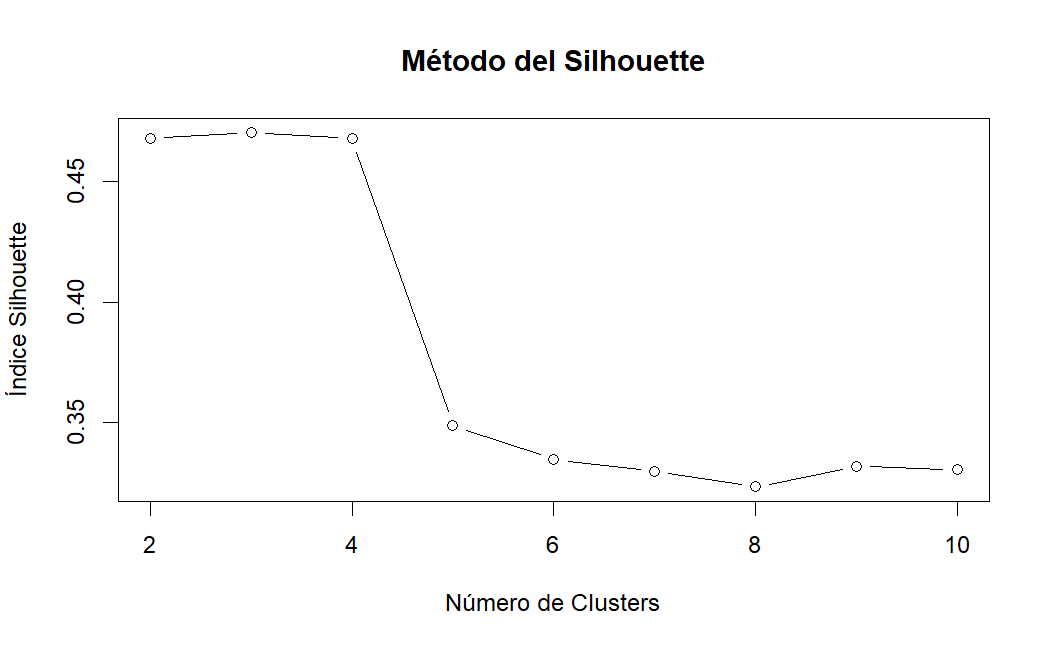
\includegraphics[width=0.8\textwidth]{figuras/Método de Silhoutte.png}
        \caption{\label{figSilhouette}Índice de Silhouette en función del número de clústeres.}
        \end{figure}
        
       
        La Tabla~\ref{figclust} presenta las medianas estandarizadas de las variables utilizadas para cada uno de los cuatro clústeres identificados. Dado que los valores corresponden a \emph{z-scores}, pueden interpretarse como desviaciones respecto a la media global del conjunto de entrenamiento.

         Por ejemplo, el valor 2.157 en la variable \textit{Monetary} para el Clúster 4 indica un nivel de gasto superior en más de dos desviaciones estándar respecto a la media, mientras que el valor -1.179 observado en el Clúster 3 refleja un gasto sustancialmente inferior al promedio.
        
        La Figura~\ref{figClusterPlot} muestra la proyección de los clústeres en el plano definido por las dos primeras componentes principales, las cuales explican conjuntamente aproximadamente el 78\% de la varianza total. La separación visual observada respalda la coherencia de la partición y la capacidad discriminante del conjunto de variables utilizadas.
        
        \begin{table}[H]
        \centering
        \caption{Medianas estandarizadas por clúster (K-means).}
        \label{figclust}
        \begin{tabular}{c c c c c c}
        \hline
        \textbf{Clúster} & \textbf{Monetary} & \textbf{Frequency} &
        \textbf{Recency} & \textbf{Descuentos} & \textbf{Cantidad} \\
        \hline
        1 & 0.855 & 1.470 & -1.349 & 0.857 & 0.676 \\
        2 & -0.430 & -0.727 & 0.541 & 0.261 & -0.515 \\
        3 & -1.179 & -0.727 & 0.673 & -2.225 & -0.090 \\
        4 & 2.157 & 1.219 & -0.417 & -2.225 & 2.301 \\
        \hline
        \end{tabular}
        \end{table}
        
       
        
        \begin{figure}[H]
        \centering
        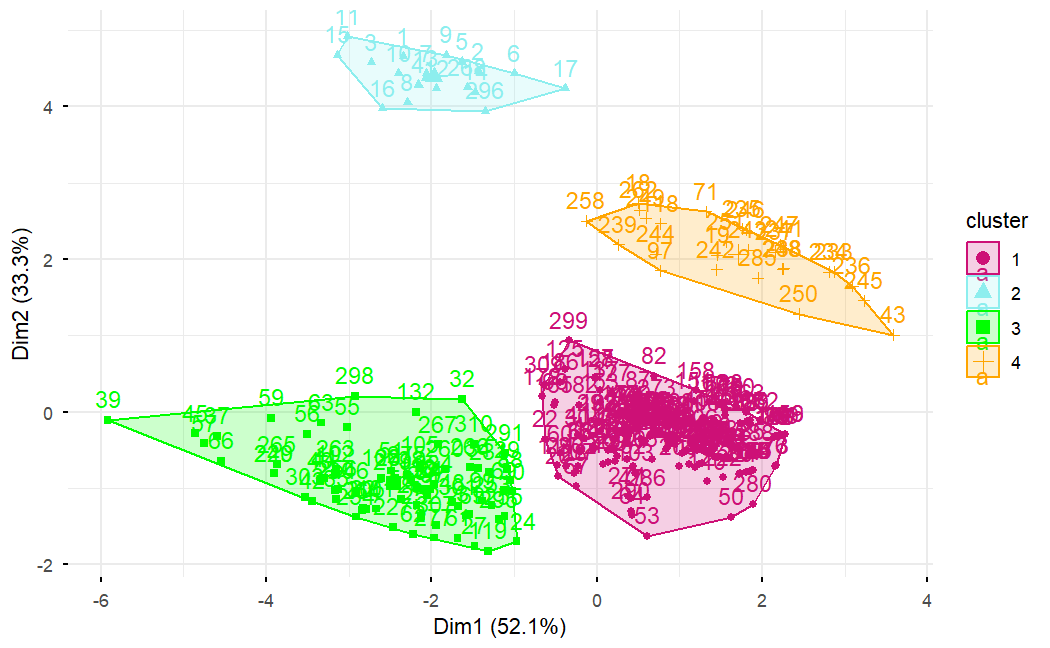
\includegraphics[width=0.8\textwidth]{figuras/Cluster Plot.png}
        \caption{\label{figClusterPlot}Proyección de los clústeres en el espacio de las dos primeras componentes principales.}
        \end{figure}
        
        A partir de los valores resumidos en la Tabla~\ref{figclust} y de la evidencia gráfica, se identifican perfiles claramente diferenciados. El Clúster 1 agrupa clientes con gasto y frecuencia superiores a la media y baja recencia, lo que indica relaciones comerciales activas y estables. El Clúster 2 concentra clientes de bajo valor, con baja frecuencia y mayor tiempo desde la última compra, representando un segmento con riesgo de abandono. El Clúster 3 presenta los niveles más bajos de gasto y frecuencia, junto con alta recencia, reflejando una relación comercial debilitada. Finalmente, el Clúster 4 se distingue por valores
        extremadamente altos de gasto, frecuencia y cantidad, baja recencia y mínima incidencia de descuentos, concentrando una proporción sustancial del valor total a pesar de su tamaño reducido, en línea con el principio de Pareto.
        
        Estos resultados confirman que el algoritmo K-means, aplicado de manera adecuada sobre variables cuantitativas y restringido al conjunto de entrenamiento, permite identificar segmentos estadísticamente diferenciados y económicamente interpretables, los cuales serán utilizados posteriormente como insumo descriptivo y como apoyo para la especificación del modelo de \emph{SoW}.

\subsection{Segmentación mediante K-medoids con distancia de Gower (variables mixtas)}
        Con el objetivo de identificar segmentos homogéneos de clientes considerando simultáneamente información transaccional y atributos categóricos, se aplicó el algoritmo de agrupación \emph{K-medoids} utilizando la distancia de Gower. Este procedimiento se implementó exclusivamente sobre el conjunto de entrenamiento, de acuerdo con el diseño experimental descrito en la sección metodológica. La
        distancia de Gower permite integrar variables continuas y cualitativas dentro de una única matriz de disimilitud, lo que resulta adecuado para la segmentación de clientes en presencia de datos mixtos.
        
        \begin{figure}[H]
        \centering
        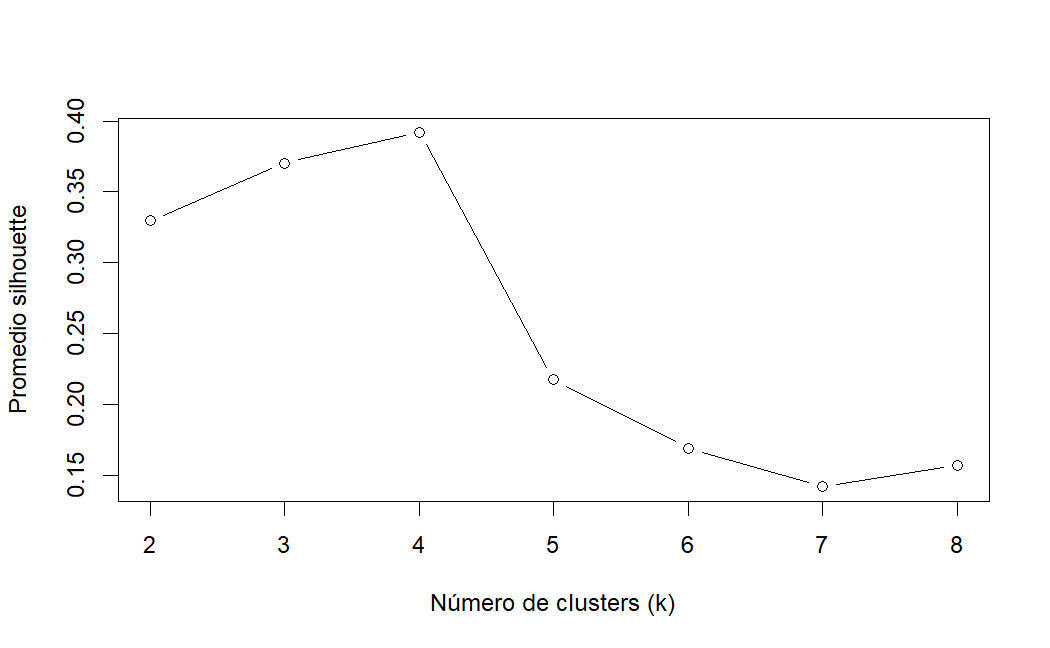
\includegraphics[width=0.8\textwidth]{figuras/Siluet.png}
        \caption{\label{figSilhouetteGower}Índice Silhouette promedio para K-medoids con distancia de Gower.}
        \end{figure}
        
        La Figura~\ref{figSilhouetteGower} presenta la evolución del índice Silhouette promedio para distintos valores del número de clústeres \(k\). Se observa que el valor máximo se alcanza en \(k = 4\), con un índice comprendido aproximadamente entre 0.39 y 0.40. A partir de este punto, el índice disminuye de forma sostenida, lo que indica una pérdida progresiva de cohesión interna y separación entre grupos al incrementar el número de clústeres. En consecuencia, la solución con cuatro clústeres se identifica como aquella que ofrece el mejor compromiso entre calidad del agrupamiento y parsimonia del modelo.
        
        Si bien estos valores son inferiores a los umbrales comúnmente asociados con estructuras de clústeres altamente definidas (superiores a 0.50), resultan consistentes con la complejidad inherente a la segmentación basada en variables mixtas. En particular, la inclusión de atributos categóricos suele reducir la separabilidad geométrica entre observaciones, lo que se refleja en valores moderados del índice Silhouette incluso cuando existe estructura latente en los
        datos.
        
        \begin{figure}[H]
        \centering
        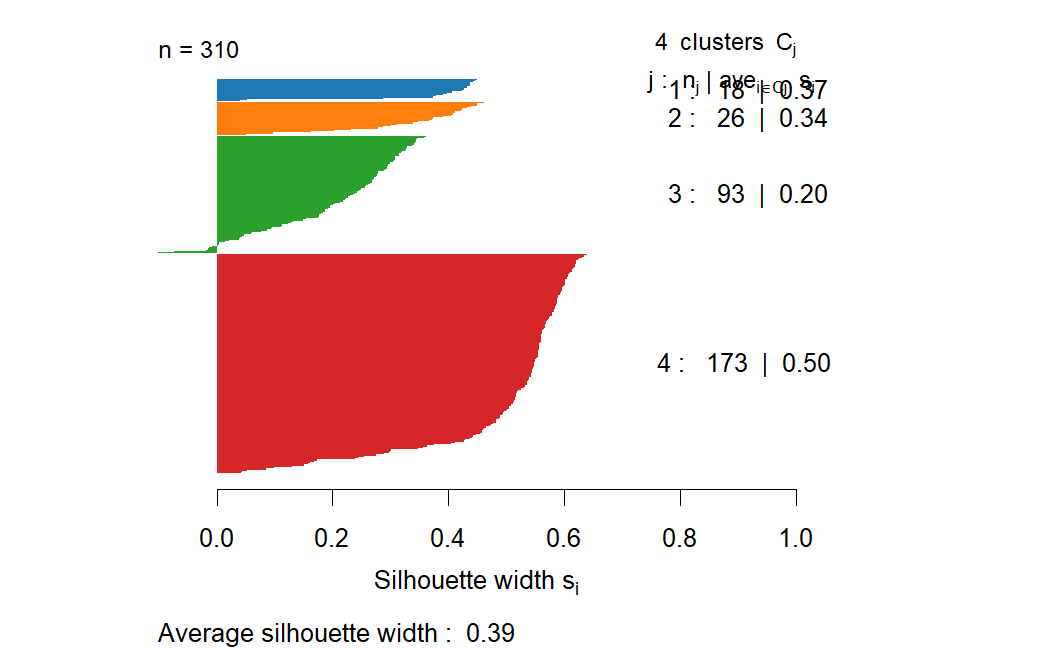
\includegraphics[width=0.8\textwidth]{figuras/KMEDOIDS.png}
        \caption{\label{figSilhouette4}Silhouette plot para la solución con \(k = 4\).}
        \end{figure}
        
        La Figura~\ref{figSilhouette4} muestra el \emph{Silhouette plot} correspondiente a la partición con cuatro clústeres. El índice Silhouette promedio global es 0.39, lo que indica una estructura de agrupamiento moderadamente consistente, aunque con heterogeneidad relevante entre los clústeres individuales.
        
        En particular, el clúster 4 presenta el mayor valor promedio de Silhouette, cercano a 0.50, lo que evidencia una elevada cohesión interna y una separación clara respecto a los demás grupos. Los clústeres 1 y 2 exhiben valores promedio de 0.37 y 0.34, respectivamente, lo que sugiere una calidad aceptable, aunque con fronteras menos definidas. En contraste, el clúster 3 presenta un valor promedio cercano a 0.20, indicando una estructura débil y un alto grado de solapamiento con
        otros clústeres, lo que sugiere una menor homogeneidad interna y una asignación menos estable de las observaciones.

        La Figura~\ref{figPAMGower} refuerza visualmente los resultados cuantitativos derivados del índice Silhouette. El clúster 4 se observa claramente compacto y bien separado, en coherencia con su alto valor promedio de Silhouette. Por el contrario, el clúster 3 presenta una dispersión considerable, consistente con su
        bajo índice de Silhouette, lo que evidencia una separación poco definida respecto a los demás grupos.
        
        Los clústeres 1 y 2, aunque de menor tamaño relativo, muestran una separación visual razonable y una dispersión moderada, lo que sugiere la existencia de segmentos de nicho caracterizados por combinaciones particulares de atributos categóricos y patrones transaccionales diferenciados.
        
        \begin{figure}[H]
        \centering
        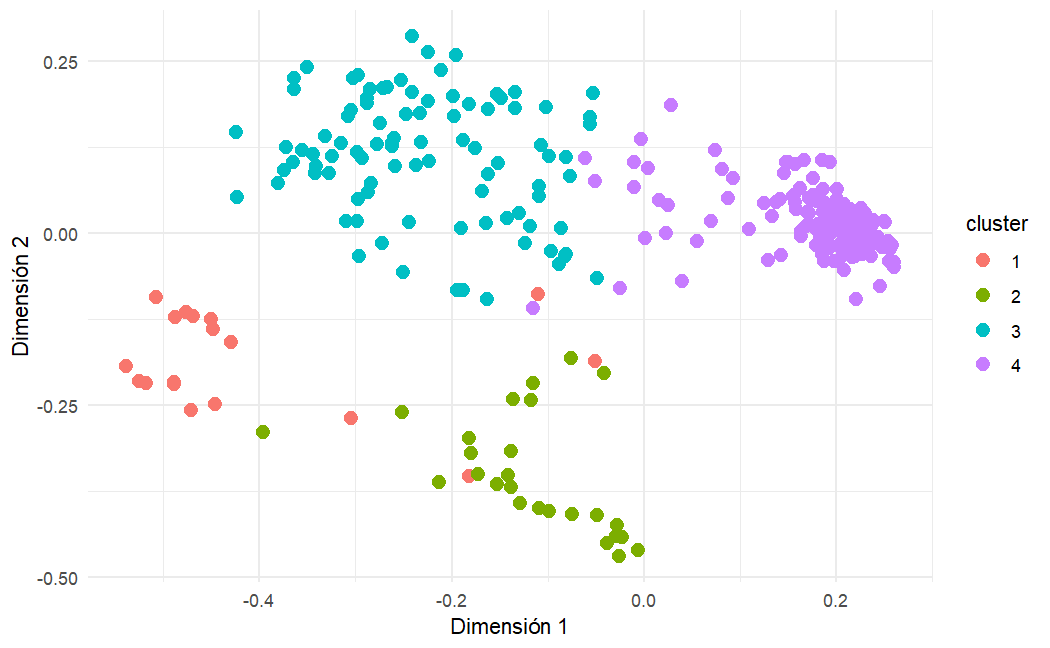
\includegraphics[width=0.8\textwidth]{figuras/CLUSTER.png}
        \caption{\label{figPAMGower}Representación bidimensional del agrupamiento PAM con distancia de Gower.}
        \end{figure}
        
        Los resultados obtenidos mediante K-medoids con distancia de Gower indican que la solución con cuatro clústeres captura una estructura relevante en los datos mixtos del conjunto de entrenamiento, permitiendo identificar segmentos con distintos niveles de cohesión y separabilidad. 

        Con el fin de evaluar la estabilidad y utilidad práctica de las segmentaciones obtenidas, los modelos de agrupamiento mediante K-means y K-medoids se aplican sobre el conjunto de prueba, asignando cada cliente a uno de los segmentos definidos a partir del conjunto de entrenamiento. Estas agrupaciones permitirán analizar la coherencia de los perfiles de clientes fuera de la muestra utilizada para la estimación, así como contrastar la segmentación basada en variables transaccionales y mixtas con la segmentación emergente del comportamiento observado. En particular, los clústeres asignados en el conjunto de prueba se compararán con la clasificación visual derivada del
        gráfico tipo \emph{bubble} de \emph{SoW} frente a
        \emph{SioW}, ambos predichos por el modelo pogit, lo que permitirá evaluar en qué medida los segmentos identificados por métodos no supervisados se alinean con patrones económicos
        predichos de participación y potencial de cartera. 

%--------------------------------------------------
\section{Resultados de la estimación del modelo \emph{pogit}}
    Esta sección presenta los resultados empíricos de la estimación del modelo \emph{pogit} aplicado al comportamiento de compra de los clientes empresariales de la Empresa Distribuidora de Biblias y Literatura Cristiana. El análisis se centra en la evidencia estadística asociada a los coeficientes estimados para los componentes de participación en la billetera (SoW) y tamaño de la billetera (SioW), así como en la consistencia de dichos resultados a través de distintas especificaciones del modelo.

    Dado el carácter latente de las variables SoW y SioW y la ausencia de valores empíricos observables de referencia, los resultados se evalúan desde una perspectiva inferencial y estructural. En particular, el énfasis se coloca en la significancia estadística, la estabilidad de los coeficientes y su coherencia con los mecanismos teóricos subyacentes al modelo \emph{pogit}, más que en criterios de validación predictiva tradicionales.

\subsection{Resultados con variables transaccionales originales}
    Las Tablas~\ref{tab:pogit_coefficients_full_version1}–\ref{tab:pogit_coefficients_version6} reportan los resultados obtenidos a partir de especificaciones del modelo \emph{pogit} construidas con variables transaccionales originales, previamente sometidas a procesos de limpieza y estandarización. En todas estas especificaciones, el componente de asignación (SoW) se modela mediante variables del tipo RFM, mientras que el componente de intensidad (SioW) incorpora distintos subconjuntos de covariables categóricas orientadas a capturar heterogeneidad estructural entre clientes.

    En el componente de participación en la billetera, la variable \textit{Monetary} exhibe coeficientes positivos en todas las especificaciones reportadas y alcanza significancia estadística en las versiones reducidas del modelo (Tablas~\ref{tab:pogit_coefficients_reduced_version3}, \ref{tab:pogit_coefficients_reduced_version4} y \ref{tab:pogit_coefficients_version5}). Este patrón indica que un mayor gasto histórico del cliente en la empresa focal se asocia sistemáticamente con una mayor fracción de su gasto total en la categoría asignada a dicha empresa, en línea con la interpretación económica de la SoW como una medida de preferencia relativa.

    Por el contrario, las variables \textit{Frequency} y \textit{Recency} no presentan efectos estadísticamente significativos en la mayoría de las especificaciones consideradas (Tablas~\ref{tab:pogit_coefficients_reduced_version3}–\ref{tab:pogit_coefficients_version6}). Este resultado sugiere que, una vez controlado el nivel agregado de gasto histórico, la frecuencia de compra y la antigüedad de la última transacción aportan información limitada para explicar la asignación relativa del gasto hacia la empresa focal.

    En el componente de intensidad (SioW), ninguna de las especificaciones basadas en variables originales presenta coeficientes individuales estadísticamente significativos, y los interceptos estimados tampoco resultan significativos en la mayoría de los casos. 

    La comparación entre la especificación completa (Tabla~\ref{tab:pogit_coefficients_full_version1}) y las versiones reducidas del modelo indica que una parametrización más parsimoniosa del componente de intensidad es suficiente para obtener estimaciones estables del componente de asignación, sin alterar de manera sustantiva los coeficientes asociados a las variables RFM en la SoW.

\subsection{Resultados con reducción de dimensionalidad mediante PCA}
    Las Tablas~\ref{tab:pogit_coefficients_version7}–\ref{tab:pogit_coefficients_version9} presentan los resultados correspondientes a especificaciones en las que el componente de asignación (SoW) se modela a partir de componentes principales obtenidas mediante Análisis de Componentes Principales (PCA).

    En las especificaciones reportadas en las Tablas~\ref{tab:pogit_coefficients_version7} y \ref{tab:pogit_coefficients_version8}, la primera componente principal (PC1) exhibe un coeficiente negativo y estadísticamente significativo en el componente SoW, mientras que la segunda componente (PC2) presenta un coeficiente positivo con significancia marginal. Este patrón sugiere que clientes con mayor intensidad económica global tienden a diversificar su gasto entre múltiples proveedores, reduciendo la fracción asignada a la empresa focal, mientras que ciertas estructuras del gasto asociadas a relaciones comerciales más específicas se vinculan con una mayor concentración del gasto en dicha empresa.

    En estas mismas especificaciones, el componente de intensidad (SioW) no presenta coeficientes individuales estadísticamente significativos, en concordancia con los resultados observados en las especificaciones basadas en variables originales.

    Un resultado cualitativamente distinto emerge en la especificación más parsimoniosa basada en PCA (Tabla~\ref{tab:pogit_coefficients_version9}). En este caso, los coeficientes asociados a las componentes principales PC1 y PC2 no resultan estadísticamente significativos en el componente de asignación (SoW). En contraste, la variable indicadora de tipo de empresa (nacional) presenta un coeficiente negativo y estadísticamente significativo en el componente de intensidad (SioW). Este resultado indica que, aun bajo una especificación mínima, persisten diferencias estructurales en el tamaño de la billetera asociadas al tipo de empresa del cliente.

    En este contexto, la pérdida de significancia de PC1 y PC2 en el componente SoW no debe interpretarse como evidencia de irrelevancia de las dimensiones latentes del comportamiento económico del cliente, sino como una limitación de dichas componentes para identificar el mecanismo de asignación cuando el componente de intensidad se encuentra altamente restringido.

\subsection{Selección de la especificación de referencia}
    Los resultados muestran que las especificaciones basadas en variables originales y aquellas que incorporan reducción de dimensionalidad mediante PCA conducen a inferencias coherentes sobre la participación en la billetera, particularmente en lo relativo al rol del gasto histórico y a la estabilidad del componente de asignación. No obstante, difieren en el grado de parsimonia y en la forma en que caracterizan el componente de intensidad.
    
    La especificación presentada en la Tabla~\ref{tab:pogit_coefficients_reduced_version3} se adopta como referencia para el análisis de estimaciones de SioW versus SoW, dado que ofrece una caracterización estable y estructural del tamaño de la billetera basada en atributos del cliente y de la categoría de producto, sin introducir dependencias estacionales ni concentrar artificialmente la heterogeneidad del componente SioW en una única variable. Esta elección proporciona una base inferencial clara y reproducible para el examen conjunto de las estimaciones de SoW y SioW en la siguiente etapa del análisis.

\begin{table}[ht]
    \centering
    \begin{threeparttable}
    \caption{Coeficientes estimados del modelo \emph{pogit} con especificación completa. Se reportan estimaciones puntuales y valores $p$ para las covariables cuantitativas del componente de participación de cartera (SoW). Las covariables categóricas incluidas en ambos componentes del modelo se estiman conjuntamente pero se omiten del reporte numérico por brevedad.}
    \label{tab:pogit_coefficients_full_version1}
    
    \begin{tabular}{
    l
    S[table-format=2.3]
    S[table-format=1.3]
    }
    \toprule
    Covariable &
    {Estimación} &
    {$p$-valor} \\
    \midrule
    
    \multicolumn{3}{l}{\textbf{SoW}}\\
    \addlinespace
    
    Intercepto
    & -5.496
    & 0.510 \\
    
    Monetary 
    & 5.676
    & 0.625 \\
    
    Frequency 
    & 0.766
    & 0.656 \\
    
    Recency 
    & -0.504
    & 0.729 \\
    
    Condiciones del cliente$^{a}$
    & {} & {} \\
    
    \addlinespace
    \midrule
    \addlinespace
    
    \multicolumn{3}{l}{\textbf{SioW}}\\
    \addlinespace
    
    Intercepto
    & -0.881
    & 0.934 \\
    
    Tipo de cliente$^{b}$
    & {} & {} \\
    
    Ubicación geográfica$^{c}$
    & {} & {} \\
    
    Categoría de producto$^{d}$
    & {} & {} \\
    
    Indicadores mensuales$^{e}$
    & {} & {} \\
    
    Tipo de empresa$^{f}$
    & {} & {} \\
    
    \bottomrule
    \end{tabular}
    
    \begin{tablenotes}[flushleft]
    \footnotesize
    \item $^{a}$ Indicadores de condición del cliente: consignación, crédito, distribuidor, donación, iglesia y librería.
    \item $^{b}$ Indicador de cliente nacional frente a internacional.
    \item $^{c}$ Variables indicadoras de departamento y ciudad (ubicaciones nacionales e internacionales).
    \item $^{d}$ Indicadores de categoría de producto: fina, línea y semifina.
    \item $^{e}$ Variables indicadoras del mes del año.
    \item $^{f}$ Indicadores de tipo de empresa: editorial, educativa, fundación y religiosa.
    \end{tablenotes}
    
    \end{threeparttable}
\end{table}


\begin{table}[ht]
    \centering
    \begin{threeparttable}
    \caption{Coeficientes estimados del modelo \emph{pogit} (Versión: SoW = Intercepto + RFM; SioW = Intercepto + Ubicación + Tipo de empresa). Se reportan las estimaciones puntuales y valores-$p$ para las covariables cuantitativas incluidas en el componente SoW. Las variables categóricas incluidas en el componente SioW se incorporan en la estimación pero se omiten del reporte numérico por brevedad.}
    \label{tab:pogit_coefficients_reduced_version2}
    
    \begin{tabular}{
    l
    S[table-format=2.3, table-number-alignment=right]
    S[table-format=1.3, table-number-alignment=right]
    }
    \toprule
    Covariable &
    {Estimación} &
    {$p$-valor} \\
    \midrule
    
    \multicolumn{3}{l}{\textbf{SoW}}\\
    \addlinespace
    
    Intercepto
    & -4.734
    & 0.005 \\
    
    Monetary
    & 5.503
    & 0.079 \\
    
    Frequency
    & 0.655
    & 0.398 \\
    
    Recency
    & -0.219
    & 0.856 \\
    
    \addlinespace
    \midrule
    \addlinespace
    
    \multicolumn{3}{l}{\textbf{SioW}}\\
    \addlinespace
    
    Intercepto
    & 0.372
    & 0.707 \\
    
    Ubicación geográfica$^{a}$
    & {} & {} \\
    
    Tipo de empresa$^{b}$
    & {} & {} \\
    
    \bottomrule
    \end{tabular}
    
\begin{tablenotes}[flushleft]
    \footnotesize
    \item $^{a}$ Variables indicadoras de ubicación geográfica a nivel de departamento y ciudad, tanto nacionales como internacionales.
    \item $^{b}$ Variables indicadoras del tipo de empresa: editorial, educativa, fundación y religiosa.
\end{tablenotes}
    
    \end{threeparttable}
\end{table}


\begin{table}[ht]
    \centering
    \begin{threeparttable}
    \caption{Coeficientes estimados del modelo \emph{pogit} (Versión: SoW = Intercepto + RFM; SioW = Intercepto + Categoría de producto + Tipo de cliente). Se reportan estimaciones puntuales y valores $p$ para las covariables cuantitativas del componente SoW. Las variables categóricas del componente de intensidad (SioW) se incluyen en la estimación pero se omiten de la presentación numérica por brevedad.}
    \label{tab:pogit_coefficients_reduced_version3}
    
    \begin{tabular}{
    l
    S[table-format=2.3]
    S[table-format=1.3]
    }
    \toprule
    Covariable &
    {Estimación} &
    {$p$-valor} \\
    \midrule
    
    \multicolumn{3}{l}{\textbf{SoW}}\\
    \addlinespace
    
    Intercepto
    & -5.144
    & 0.000 \\
    
    Monetary
    & 4.681
    & 0.003 \\
    
    Frequency
    & 0.687
    & 0.199 \\
    
    Recency
    & -0.053
    & 0.955 \\
    
    \addlinespace
    \midrule
    \addlinespace
    
    \multicolumn{3}{l}{\textbf{SioW}}\\
    \addlinespace
    
    Intercepto
    & 0.430
    & 0.414 \\
    
    Tipo de cliente / empresa$^{a}$
    & {} & {} \\
    
    Categoría de producto$^{b}$
    & {} & {} \\
    
    \bottomrule
    \end{tabular}
    
    \begin{tablenotes}[flushleft]
    \footnotesize
    \item $^{a}$ Indicadores del tipo de cliente y tipo de empresa: cliente nacional e indicadores de empresa (editorial, educativa, fundación, religiosa).
    \item $^{b}$ Indicadores de categoría de producto: fina, línea y semifina.
    \end{tablenotes}
    
    \end{threeparttable}
\end{table}

\begin{table}[ht]
    \centering
    \begin{threeparttable}
    \caption{Coeficientes estimados del modelo \emph{pogit} (Versión: SoW = Intercepto + RFM; SioW = Intercepto + Categoría de producto + Mes del año). Se reportan estimaciones puntuales y valores $p$ para las covariables cuantitativas del componente de participación de cartera (SoW). Las variables categóricas y estacionales del componente de intensidad (SioW) se incluyen en la estimación pero se omiten del reporte numérico por brevedad.}
    \label{tab:pogit_coefficients_reduced_version4}
    
    \begin{tabular}{
    l
    S[table-format=2.3]
    S[table-format=1.3]
    }
    \toprule
    Covariable &
    {Estimación} &
    {$p$-valor} \\
    \midrule
    
    \multicolumn{3}{l}{\textbf{SoW}}\\
    \addlinespace
    
    Intercepto
    & -4.834
    & 0.000 \\
    
    Monetary
    & 5.262
    & 0.001 \\
    
    Frequency
    & 0.598
    & 0.172 \\
    
    Recency
    & 0.130
    & 0.873 \\
    
    \addlinespace
    \midrule
    \addlinespace
    
    \multicolumn{3}{l}{\textbf{SioW}}\\
    \addlinespace
    
    Intercepto
    & 0.804
    & 0.084 \\
    
    Categoría de producto$^{a}$
    & {} & {} \\
    
    Mes del año$^{b}$
    & {} & {} \\
    
    \bottomrule
    \end{tabular}
    
    \begin{tablenotes}[flushleft]
    \footnotesize
    \item $^{a}$ Indicadores de categoría de producto: fina, línea y semifina.
    \item $^{b}$ Indicadores mensuales: enero a diciembre (estacionalidad anual).
    \end{tablenotes}
    
    \end{threeparttable}
\end{table}

\begin{table}[ht]
    \centering
    \begin{threeparttable}
    \caption{Coeficientes estimados del modelo \emph{pogit} (Versión: SoW = Intercepto + RFM; SioW = Intercepto + Categoría de producto). Se reportan estimaciones puntuales y valores $p$ para las covariables cuantitativas del componente de participación de cartera (SoW). Las covariables categóricas incluidas en ambos componentes del modelo se estiman conjuntamente pero se omiten del reporte numérico por brevedad.}
    \label{tab:pogit_coefficients_version5}
    
    \begin{tabular}{
    l
    S[table-format=2.3]
    S[table-format=1.3]
    }
    \toprule
    Covariable &
    {Estimación} &
    {$p$-valor} \\
    \midrule
    
    \multicolumn{3}{l}{\textbf{SoW}}\\
    \addlinespace
    
    Intercepto
    & -4.126
    & 0.004 \\
    
    Monetary
    & 6.305
    & 0.010 \\
    
    Frequency
    & 0.440
    & 0.466 \\
    
    Recency
    & -0.019
    & 0.984 \\
    
    \addlinespace
    \midrule
    \addlinespace
    
    \multicolumn{3}{l}{\textbf{SioW}}\\
    \addlinespace
    
    Intercepto
    & -0.603
    & 0.550 \\
    
    Categoría de producto$^{a}$
    & {} & {} \\
    
    \bottomrule
    \end{tabular}
    
    \begin{tablenotes}[flushleft]
    \footnotesize
    \item $^{a}$ Indicadores de categoría de producto: fina, línea y semifina.
    \end{tablenotes}
    
    \end{threeparttable}
\end{table}


\begin{table}[ht]
    \centering
    \begin{threeparttable}
    \caption{Coeficientes estimados del modelo \emph{pogit} (Versión: SoW = Intercepto + RFM; SioW = Intercepto + indicadores mensuales). Se reportan estimaciones puntuales y valores $p$ para las covariables cuantitativas del componente de participación de cartera (SoW). Las covariables categóricas del componente de intensidad (SioW) se estiman conjuntamente pero se omiten del reporte numérico por brevedad.}
    \label{tab:pogit_coefficients_version6}
    
    \begin{tabular}{
    l
    S[table-format=2.3]
    S[table-format=1.3]
    }
    \toprule
    Covariable &
    {Estimación} &
    {$p$-valor} \\
    \midrule
    
    \multicolumn{3}{l}{\textbf{SoW}}\\
    \addlinespace
    
    Intercepto
    & -4.834
    & 0.000 \\
    
    Monetary
    & 5.262
    & 0.001 \\
    
    Frequency
    & 0.598
    & 0.172 \\
    
    Recency
    & 0.130
    & 0.873 \\
    
    \addlinespace
    \midrule
    \addlinespace
    
    \multicolumn{3}{l}{\textbf{SioW}}\\
    \addlinespace
    
    Intercepto
    & 0.804
    & 0.084 \\
    
    Indicadores mensuales$^{a}$
    & {} & {} \\
    
    \bottomrule
    \end{tabular}
    
    \begin{tablenotes}[flushleft]
    \footnotesize
    \item $^{a}$ Variables indicadoras del mes del año.
    \end{tablenotes}
    
    \end{threeparttable}
\end{table}


\begin{table}[ht]
    \centering
    \begin{threeparttable}
    \caption{Coeficientes estimados del modelo \emph{pogit} (Versión: SoW = Intercepto + PC1 + PC2 + condiciones del cliente; SioW = Intercepto + Ubicación geográfica + Tipo de empresa). Se reportan las estimaciones puntuales y valores-$p$ para las covariables cuantitativas incluidas en el componente SoW. Las variables categóricas del componente SioW se incorporan en la estimación pero se omiten del reporte numérico por brevedad.}
    \label{tab:pogit_coefficients_version7}
    
    \begin{tabular}{
    l
    S[table-format=2.3, table-number-alignment=right]
    S[table-format=1.3, table-number-alignment=right]
    }
    \toprule
    Covariable &
    {Estimación} &
    {$p$-valor} \\
    \midrule
    
    \multicolumn{3}{l}{\textbf{SoW}}\\
    \addlinespace
    
    Intercepto
    & -5.167
    & 0.000 \\
    
    PC1
    & -2.997
    & 0.005 \\
    
    PC2
    & 2.066
    & 0.053 \\
    
    Condición: consignación
    & -0.468
    & 0.987 \\
    
    Condición: crédito
    & 1.793
    & 0.271 \\
    
    Condición: distribuidor
    & -8.612
    & 0.960 \\
    
    \addlinespace
    \midrule
    \addlinespace
    
    \multicolumn{3}{l}{\textbf{SioW}}\\
    \addlinespace
    
    Intercepto
    & 0.367
    & 0.068 \\
    
    Ubicación geográfica$^{a}$
    & {} & {} \\
    
    Tipo de empresa$^{b}$
    & {} & {} \\
    
    \bottomrule
    \end{tabular}
    
    \begin{tablenotes}[flushleft]
    \footnotesize
    \item $^{a}$ Variables indicadoras de ubicación geográfica agregada.
    \item $^{b}$ Indicadores de tipo de empresa.
    \end{tablenotes}
    
    \end{threeparttable}
\end{table}


\begin{table}[ht]
    \centering
    \begin{threeparttable}
    \caption{Coeficientes estimados del modelo \emph{pogit} (Versión: SoW = Intercepto + PC1 + PC2 + condiciones del cliente; SioW = Intercepto + Ubicación geográfica + Tipo de empresa + Categoría de producto). Se reportan las estimaciones puntuales y valores-$p$ para las covariables cuantitativas incluidas en el componente SoW. Las variables categóricas del componente SioW se incorporan en la estimación pero se omiten del reporte numérico por brevedad.}
    \label{tab:pogit_coefficients_version8}
    
    \begin{tabular}{
    l
    S[table-format=2.3, table-number-alignment=right]
    S[table-format=1.3, table-number-alignment=right]
    }
    \toprule
    Covariable &
    {Estimación} &
    {$p$-valor} \\
    \midrule
    
    \multicolumn{3}{l}{\textbf{SoW}}\\
    \addlinespace
    
    Intercepto
    & -5.083
    & 0.000 \\
    
    PC1
    & -3.163
    & 0.009 \\
    
    PC2
    & 2.243
    & 0.074 \\
    
    Condición: consignación
    & -0.446
    & 0.987 \\
    
    Condición: crédito
    & 1.885
    & 0.282 \\
    
    Condición: distribuidor
    & -8.752
    & 0.987 \\
    
    \addlinespace
    \midrule
    \addlinespace
    
    \multicolumn{3}{l}{\textbf{SioW}}\\
    \addlinespace
    
    Intercepto
    & 0.437
    & 0.437 \\
    
    Ubicación geográfica$^{a}$
    & {} & {} \\
    
    Tipo de empresa$^{b}$
    & {} & {} \\
    
    Categoría de producto$^{c}$
    & {} & {} \\
    
    \bottomrule
    \end{tabular}
    
    \begin{tablenotes}[flushleft]
    \footnotesize
    \item $^{a}$ Variables indicadoras de ubicación geográfica agregada.
    \item $^{b}$ Indicadores de tipo de empresa.
    \item $^{c}$ Indicadores de categoría de producto.
    \end{tablenotes}
    
    \end{threeparttable}
\end{table}

\begin{table}[ht]
    \centering
    \begin{threeparttable}
    \caption{Coeficientes estimados del modelo \emph{pogit} (Versión: SoW = Intercepto + PC1 + PC2; SioW = Intercepto + Tipo de empresa). Se reportan las estimaciones puntuales y valores-$p$ para las covariables cuantitativas incluidas en el componente SoW. La variable categórica incluida en el componente SioW se incorpora en la estimación pero se reporta únicamente su coeficiente agregado.}
    \label{tab:pogit_coefficients_version9}
    
    \begin{tabular}{
    l
    S[table-format=2.3, table-number-alignment=right]
    S[table-format=1.3, table-number-alignment=right]
    }
    \toprule
    Covariable &
    {Estimación} &
    {$p$-valor} \\
    \midrule
    
    \multicolumn{3}{l}{\textbf{SoW}}\\
    \addlinespace
    
    Intercepto
    & -4.010
    & 0.288 \\
    
    PC1
    & -4.304
    & 0.339 \\
    
    PC2
    & 1.854
    & 0.655 \\
    
    \addlinespace
    \midrule
    \addlinespace
    
    \multicolumn{3}{l}{\textbf{SioW}}\\
    \addlinespace
    
    Intercepto
    & 0.223
    & 0.387 \\
    
    Tipo de empresa (nacional)$^{a}$
    & -1.790
    & 0.017 \\
    
    \bottomrule
    \end{tabular}
    
    \begin{tablenotes}[flushleft]
    \footnotesize
    \item $^{a}$ Variable indicadora de tipo de empresa; la categoría de referencia corresponde a empresas no nacionales.
    \end{tablenotes}
    
    \end{threeparttable}
\end{table}

    
%--------------------------------------------------
\subsection{Algoritmos de agrupación versus segmentación SioW vs. SoW}

    La Figura~\ref{fig:sow_siow_kmeans} presenta el plano SoW--SioW para el conjunto de prueba, con los clientes coloreados según los clústeres obtenidos mediante k-means. Se observa que el clúster C2 tiende a presentar los valores relativamente más altos de
    \emph{SoW} dentro de la muestra, constituyendo el único grupo que exhibe una diferenciación apreciable en el eje horizontal, aunque los niveles absolutos de participación permanecen moderados.
    
    En contraste, los clústeres C1, C3 y C4 muestran una superposición sustancial en el eje SoW y se distinguen principalmente por la dispersión vertical asociada al
    \emph{SioW}. En particular, el clúster C3 agrupa un subconjunto reducido de clientes con baja participación y valores de SioW relativamente elevados y concentrados, mientras que el clúster C4 presenta una heterogeneidad considerable en SioW, abarcando desde niveles medios hasta los valores más altos observados en la
    muestra.
    
    Estos resultados indican que la segmentación no supervisada basada en
    variables transaccionales originales no induce una partición clara del espacio latente SoW--SioW, salvo por una diferenciación relativa asociada a mayores niveles de participación. Esto sugiere que los clústeres capturan regularidades parciales del
    comportamiento observado, pero no reproducen directamente la estructura latente inferida por el modelo \emph{pogit}.

    En la Figura~\ref{fig:sow_siow_kmedoids} se observa que la segmentación mediante k-medoids, basada en variables mixtas, no induce una partición estricta del plano SoW--SioW, sino que organiza los clientes principalmente según patrones de
    heterogeneidad en el \emph{SioW} latente.

    El clúster C3 destaca como el único grupo claramente concentrado, compuesto por clientes con valores elevados de SioW y participación prácticamente nula, lo que sugiere la existencia de un segmento estructuralmente homogéneo en términos de potencial latente. En contraste, los clústeres C2 y C4 presentan una dispersión
    vertical considerable, agrupando clientes con tamaños de billetera latente que abarcan desde niveles medios hasta altos, mientras que C1 concentra clientes con SioW relativamente bajo y variabilidad limitada.
    
    Estos resultados sugieren que, aunque la segmentación basada en variables mixtas permite explorar regularidades estructurales en los datos observados, la heterogeneidad en el potencial de cartera no siempre se traduce en clústeres compactos
    en el espacio SoW--SioW. Esto refuerza el rol del modelo \emph{pogit} como herramienta principal de inferencia latente, y a los métodos de clustering como instrumentos
    complementarios de análisis exploratorio y validación estructural.


    \begin{figure}[H]
    \centering
    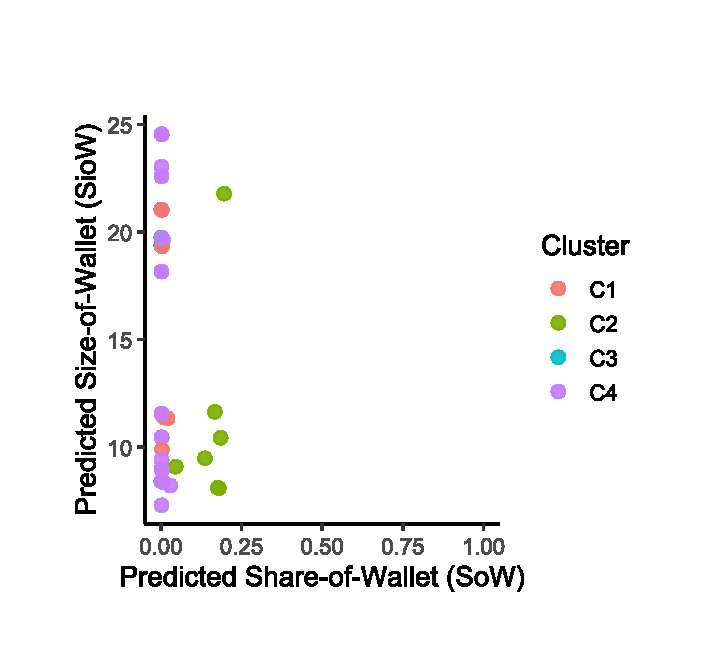
\includegraphics[width=0.75\textwidth]{figuras/sow-siow-k-means.pdf}
    \caption{Plano SoW--SioW para el conjunto de prueba. 
    Cada punto representa un cliente, coloreado según el clúster obtenido mediante \emph{k-means}. 
    El eje horizontal corresponde a la \emph{Share-of-Wallet} (SoW) predicha y el eje vertical a la 
    \emph{Size-of-Wallet} (SioW) predicha por el modelo \emph{pogit}.}
    \label{fig:sow_siow_kmeans}
\end{figure}


 \begin{figure}[H]
    \centering
    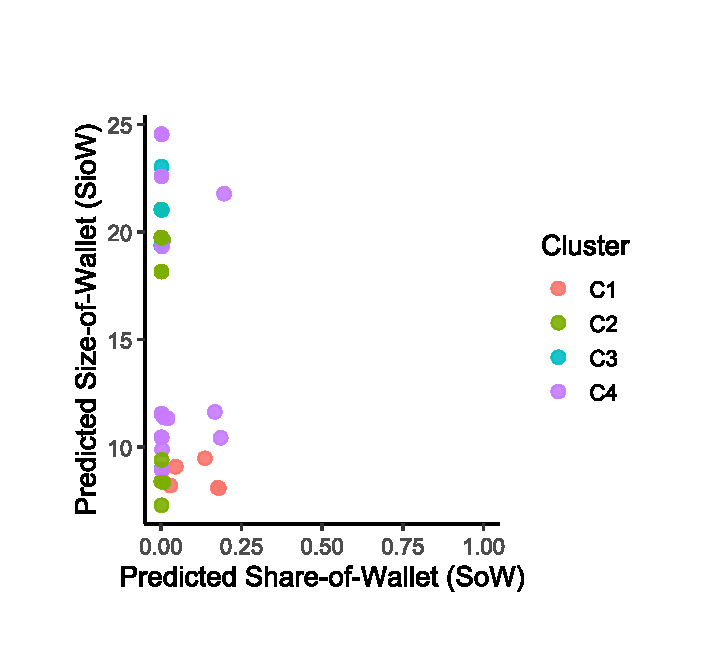
\includegraphics[width=0.75\textwidth]{figuras/sow-siow-k-mdd.pdf}
    \caption{Plano SoW--SioW para el conjunto de prueba. 
    Cada punto representa un cliente, coloreado según el clúster obtenido mediante \emph{k-medoids}. 
    El eje horizontal corresponde a la \emph{Share-of-Wallet} (SoW) predicha y el eje vertical a la 
    \emph{Size-of-Wallet} (SioW) predicha por el modelo \emph{pogit}.}
    \label{fig:sow_siow_kmedoids}
\end{figure}

    
    
        
    

     % --------------------------
    \chapter{Discusión y Trabajo Futuro}
    
%--------------------------------------------------
\section{Discusión}

El principal aporte de este trabajo radica en la estimación de la \emph{participación en la billetera} (SoW) y del \emph{tamaño de la billetera} (SioW) en un contexto de información parcial, característico de aplicaciones empresariales reales. En particular, la empresa focal no observa el gasto total de sus clientes en la categoría ni dispone de información directa sobre transacciones realizadas con competidores o de medidas de intención de compra obtenidas mediante encuestas. En este escenario, el modelo \emph{pogit} no se concibe como un mecanismo de predicción directa de variables observables, sino como una herramienta de inferencia estructural que permite reconstruir cantidades latentes coherentes con los patrones transaccionales disponibles.

La aplicación del modelo al segmento de clientes empresariales resulta especialmente pertinente, dado que el entorno B2B presenta dinámicas de compra sustancialmente distintas a las del consumo final. Las compras empresariales suelen caracterizarse por frecuencias relativamente bajas, montos agregados elevados y estructuras de pedido complejas asociadas a descuentos por volumen y relaciones comerciales de largo plazo. En este contexto, la descomposición del gasto observado en un componente de intensidad latente (SioW) y un componente de asignación (SoW) permite distinguir entre el potencial económico total del cliente y el grado en que dicho potencial es capturado por la empresa focal, aportando una lectura económica más rica que la que se obtiene a partir de métricas tradicionales de facturación.

La representación conjunta de las estimaciones ajustadas de SoW y SioW en el plano bidimensional facilita la identificación de perfiles de clientes con implicaciones estratégicas diferenciadas. En particular, se observan clientes con alto SioW y bajo SoW, que representan oportunidades de crecimiento en participación; clientes con bajo SioW y alto SoW, caracterizados por una relación estable pero de alcance económico limitado; y clientes con valores elevados en ambas dimensiones, que constituyen el núcleo estratégico de la cartera. Esta segmentación inducida por el modelo proporciona una base interpretable para la priorización de acciones comerciales y de retención.

Las técnicas de segmentación no supervisada empleadas —k-means y k-medoids— cumplen un rol complementario como herramientas de validación estructural e interpretabilidad. La correspondencia observada entre los clusters definidos a partir de variables transaccionales y las regiones emergentes del espacio SoW--SioW sugiere que las estimaciones del modelo capturan patrones consistentes con agrupaciones naturales de clientes basadas en información observable. Este ejercicio no constituye una validación predictiva en sentido estricto, sino una evaluación de coherencia económica y estabilidad estructural fuera de muestra, adecuada para un modelo cuyos principales objetos de interés son variables latentes no observables directamente.

Finalmente, la comparación entre una especificación del modelo basada en variables transaccionales originales y una alternativa basada en reducción de dimensionalidad mediante PCA pone de manifiesto un trade--off entre parsimonia estadística e interpretabilidad de negocio. Mientras que el uso de componentes principales contribuye a la estabilidad numérica y a la reducción de colinealidad, la especificación con variables originales facilita la traducción directa de los resultados en decisiones operativas. Ambas aproximaciones resultan complementarias y su elección depende del objetivo analítico específico.

%--------------------------------------------------
\section{Trabajos futuros}

Una primera línea de extensión de este trabajo consiste en aplicar la metodología propuesta al segmento de personas naturales. A diferencia de los clientes empresariales, los consumidores finales presentan patrones de compra con mayor frecuencia relativa, menor monto por transacción y una mayor sensibilidad a promociones y estímulos comerciales. Evaluar el desempeño del modelo \emph{pogit} en este contexto permitiría analizar su grado de generalidad y comparar sistemáticamente las distribuciones de SoW y SioW entre segmentos B2B y B2C.

Una segunda extensión metodológica relevante corresponde al desarrollo de modelos que integren simultáneamente clientes empresariales y personas naturales dentro de un mismo marco analítico. Esto podría abordarse mediante modelos de mezcla finita o especificaciones jerárquicas que permitan parámetros diferenciados para los mecanismos de asignación e intensidad según el tipo de cliente. Dichos enfoques permitirían capturar heterogeneidad estructural sin necesidad de estimar modelos completamente separados, manteniendo coherencia estadística y mejorando la eficiencia inferencial.

Otra línea de investigación consiste en incorporar explícitamente la dimensión temporal del comportamiento de compra. La estimación del modelo en ventanas móviles o la inclusión de componentes dinámicos permitiría estudiar la estabilidad temporal de la SoW y del SioW, identificar trayectorias de crecimiento o deterioro en la relación con la empresa focal y diseñar mecanismos de alerta temprana frente a pérdidas potenciales de participación en la billetera.

Desde el punto de vista estadístico, futuros trabajos podrían explorar extensiones distribucionales del componente de intensidad, tales como modelos Poisson--Gamma o binomial negativa, con el fin de capturar posibles fenómenos de sobredispersión no modelados explícitamente en la especificación actual. Estas extensiones permitirían evaluar la robustez de los resultados frente a supuestos distribucionales más flexibles, manteniendo la estructura conceptual del modelo.

Finalmente, las estimaciones de SoW y SioW obtenidas podrían integrarse en marcos de análisis causal o de \emph{uplift modeling} para evaluar el impacto de intervenciones comerciales específicas, como campañas promocionales, cambios en condiciones de descuento o estrategias de fidelización. Esta integración permitiría avanzar desde un análisis descriptivo e inferencial hacia herramientas prescriptivas orientadas a la optimización de decisiones de marketing y a la gestión estratégica del valor del cliente.


   % --------------------------
    \chapter{Conclusiones}
    %--------------------------------------------------


\section{Conclusión asociada al objetivo general}

El objetivo general de este trabajo fue desarrollar una metodología de ciencia de datos, basada en información transaccional parcial, para estimar la \emph{participación en la billetera} (\emph{Share--of--Wallet}, SoW) y el \emph{tamaño de la billetera} (\emph{Size--of--Wallet}, SioW) de clientes empresariales de una empresa distribuidora de biblias y literatura cristiana, en ausencia de información proveniente de encuestas o de transacciones con empresas competidoras.

Los resultados obtenidos permiten concluir que este objetivo fue alcanzado de manera satisfactoria. La metodología propuesta posibilita la inferencia de cantidades latentes económica y estadísticamente coherentes a partir de datos internos, mediante un modelo jerárquico \emph{pogit} que separa explícitamente el mecanismo de asignación del gasto hacia la empresa focal del mecanismo de intensidad total de consumo en la categoría. Esta estructura resulta especialmente adecuada para contextos B2B reales, donde la información disponible es inherentemente incompleta y limitada al portafolio de ventas de la empresa focal.

%--------------------------------------------------
\section{Conclusión asociada al objetivo específico 1}

El primer objetivo específico consistió en identificar las variables transaccionales y de perfilamiento del cliente relevantes para explicar la SoW y el SioW de los clientes empresariales, utilizando exclusivamente información observable.

Los resultados muestran que ambos tipos de variables cumplen funciones diferenciadas y complementarias dentro del modelo. Las variables transaccionales —como recencia, frecuencia, gasto monetario, diversidad de productos y regularidad del consumo. Las variables transaccionales resultan particularmente informativas en términos estructurales para explicar el mecanismo de asignación del gasto hacia la empresa focal (SoW), aun cuando no todas ellas exhiben efectos marginales estadísticamente significativos de manera individual. En contraste, las variables de perfilamiento, como el tipo de empresa y la zona geográfica, capturan heterogeneidad estructural asociada al tamaño total de la billetera del cliente en la categoría (SioW). Esta evidencia respalda empíricamente la separación conceptual entre ambos mecanismos y justifica el uso de matrices de covariables diferenciadas en la especificación del modelo.

%--------------------------------------------------
\section{Conclusión asociada al objetivo específico 2}

El segundo objetivo específico buscó comparar distintas especificaciones del conjunto de covariables transaccionales utilizadas en el modelo \emph{pogit}, incluyendo una especificación basada en variables originales y una alternativa basada en reducción de dimensionalidad mediante Análisis de Componentes Principales (PCA).

Se concluye que ambas especificaciones presentan ventajas complementarias. La especificación basada en variables originales ofrece una interpretación directa y facilita la traducción de los resultados en acciones comerciales concretas. Por su parte, la especificación basada en PCA proporciona mayor parsimonia y estabilidad numérica, al sintetizar la información contenida en variables altamente correlacionadas. En consecuencia, la elección entre ambas especificaciones depende del objetivo analítico —interpretabilidad o simplificación del modelo— más que de un criterio único de desempeño, lo que refuerza la flexibilidad metodológica del enfoque propuesto.

%--------------------------------------------------
\section{Conclusión asociada al objetivo específico 3}

El tercer objetivo específico se orientó a analizar la estructura de segmentación de los clientes obtenida mediante técnicas de aprendizaje no supervisado y su correspondencia con los patrones emergentes en el espacio conjunto SoW--SioW estimado por el modelo \emph{pogit}.

Los resultados indican que los métodos de segmentación empleados (k-means y k-medoids) permiten identificar grupos de clientes con perfiles observables homogéneos y patrones consistentes —aunque no perfectamente separables— en términos de participación e intensidad de gasto estimadas. La correspondencia observada entre los segmentos derivados de variables transaccionales y las regiones emergentes del espacio SoW--SioW aporta evidencia adicional de la coherencia estructural del modelo fuera de muestra. Este análisis confirma que la segmentación no supervisada constituye una herramienta útil para apoyar la interpretación económica de las estimaciones del modelo, sin intervenir directamente en su proceso de estimación.























% El presente trabajo tuvo como propósito central desarrollar y validar una metodología para estimar el \textit{Share of Wallet} (SoW) de los clientes de la Sociedad Bíblica Colombiana (SBC), a partir de información transaccional y de perfilamiento, evitando la dependencia exclusiva de encuestas declarativas. La contribución se inscribe en la línea propuesta por Glady \& Croux \cite{glady2009predicting} y en la literatura sobre Wallet Allocation Rule (WAR) y métricas de satisfacción–participación, integrando dichos marcos conceptuales en un contexto B2B específico de distribución de literatura cristiana.

% \subsection{Síntesis metodológica y coherencia con el marco teórico}

% En primer lugar, se destaca la coherencia lograda entre el marco conceptual, la metodología propuesta y los resultados obtenidos. La metodología implementada siguió las etapas definidas en la sección de Metodología (\ref{sec:metodologia}), que abarcan: (i) pre-procesamiento y depuración de datos, (ii) análisis exploratorio univariado y multivariado, (iii) transformación logarítmica y estandarización, (iv) reducción de dimensionalidad mediante PCA, (v) segmentación por K-means y K-medoids con distancia de Gower, (vi) construcción de las matrices transaccional \(\mathbf{W}\) y de perfilamiento \(\mathbf{V}\), (vii) definición de la variable respuesta discreta a partir del gasto monetario, y (viii) estimación del SoW mediante un modelo compuesto tipo GBinM (Glady \& Croux) y modelos comparadores (GLM/Tweedie, GAM con splines).

% En términos formales, la estrategia se apoyó en la representación del gasto total del cliente (\(W_i\)) y de la participación de la SBC en dicho gasto (\(\mathrm{SoW}_i\)), cuyas definiciones y formulaciones se presentan en el Marco Teórico (\ref{sec:marco-teorico}, subsecciones sobre ``Conceptos formales y notación'' y ``Wallet Allocation Rule (visión conceptual y operacional)''). En lugar de incluir las expresiones matemáticas completas en el cuerpo de las conclusiones, se hace referencia explícita a dichas ecuaciones, donde se detalla la forma funcional de \(\mathrm{SoW}_i\), \(\mathrm{PoW}_i\) y del gasto total estimado \(\widehat{W}_i\).

% Asimismo, el modelo compuesto adoptado —basado en la factorización de la media \(\mu_i\) en una componente de escala (\(\lambda_i\)) y una componente de asignación o preferencia (\(\pi_i\))— sigue la propuesta original de Glady \& Croux y se encuentra formalizado en el Marco Teórico (\ref{sec:marco-teorico}, subsección ``Modelos para estimar SioW y SoW: enfoque de dos componentes'') y detallado en la Metodología. En dichas secciones se presentan las ecuaciones que describen: (i) la distribución de la variable discreta de respuesta \(Y_i\) que aproxima el gasto monetario, (ii) la forma de las funciones de enlace que relacionan \(\lambda_i\) con \(\mathbf{W}_i\) y \(\pi_i\) con \(\mathbf{V}_i\), y (iii) la manera en que, a partir de \(\widehat{\lambda}_i\) y \(\widehat{\pi}_i\), se obtienen los estimadores de \(W_i\), \(\mathrm{SoW}_i\) y \(\mathrm{PoW}_i\).

% Esta separación explícita entre el desarrollo matemático (ubicado en el Marco Teórico) y la interpretación empírica (ubicada en Resultados y Conclusiones) atiende la recomendación de la profesora acerca de centralizar las fórmulas en un solo apartado y garantiza consistencia y trazabilidad conceptual en todo el documento.

% \subsection{Hallazgos sobre SioW, SoW y potencial de wallet (PoW)}

% En segundo lugar, los resultados permiten concluir que la metodología propuesta es capaz de generar estimaciones razonables y accionables del SoW y del potencial de wallet (PoW) de los clientes de la SBC, sin recurrir a datos declarativos de encuestas. El componente observacional de desempeño (\(\mathrm{SioW}\)) —definido y formalizado también en el Marco Teórico (\ref{sec:marco-teorico})— se derivó directamente del comportamiento histórico de compra, lo que permitió medir la participación efectiva de la SBC en el gasto realizado, mientras que el componente esperado (\(\mathrm{SoW}\)) se obtuvo a partir de la estructura del modelo compuesto.

% En particular, la variable discreta de respuesta \(Y_i\) se construyó a partir del valor monetario total del cliente (\(Y2_i\)) en el periodo de evaluación (año 2024), utilizando una constante de escala \(C\) basada en la razón entre la varianza y la media de dicho gasto, siguiendo la lógica descrita por Glady \& Croux. La fórmula utilizada para \(C\) y para \(Y_i\) se presenta íntegramente en el Marco Teórico y en la Metodología, de forma que cualquier lector pueda verificar paso a paso la transformación aplicada. Este procedimiento permitió llevar un gasto continuo con fuerte asimetría a una variable de conteo más adecuada para la parte Poisson del modelo compuesto.

% A partir de las estimaciones de \(\widehat{W}_i\) y \(\widehat{\mathrm{SoW}}_i\), se derivó \(\widehat{\mathrm{PoW}}_i\), entendida como el potencial de wallet no capturado por la SBC. Formalmente, la relación entre estas magnitudes se detalla en las ecuaciones respectivas del Marco Teórico, mientras que en esta sección se enfatiza la interpretación: clientes con alta \(\widehat{\mathrm{PoW}}_i\) representan oportunidades claras para incrementar ingresos sin necesidad de adquirir nuevos clientes, simplemente profundizando la relación con quienes ya son compradores actuales.

% Los resultados muestran, además, la presencia de un patrón de tipo Pareto en el portafolio de clientes, donde un subconjunto reducido concentra una fracción desproporcionada del wallet y del PoW, coherente con lo observado en el análisis exploratorio de variables monetarias y de cantidad. Este hallazgo refuerza la utilidad de las estimaciones de SoW para identificar clientes de alto impacto potencial y para priorizar acciones comerciales de manera más estratégica.

% \subsection{Desempeño de los modelos y comparación de especificaciones}

% En tercer lugar, el desempeño del modelo compuesto se contrastó con el de modelos alternativos (GLM/Tweedie y modelos con splines), utilizando métricas tales como el error absoluto medio (MAE) y la raíz del error cuadrático medio (RMSE), cuyas definiciones se encuentran en el Marco Teórico (\ref{sec:marco-teorico}, subsección ``Validación, métricas y criterios operativos''). Esta decisión fue coherente con el objetivo de evaluar no solo la capacidad explicativa, sino también la calidad predictiva del enfoque propuesto.

% En términos generales, el modelo compuesto basado en \(\mathbf{W}\) y \(\mathbf{V}\) mostró un desempeño competitivo, particularmente en la estimación de \(\widehat{W}_i\) y \(\widehat{\mathrm{SoW}}_i\), frente a alternativas más simples basadas en modelos lineales generalizados. La inclusión de una componente de asignación \(\pi_i\) vinculada a variables de perfilamiento (matriz \(\mathbf{V}\)) aportó flexibilidad adicional para capturar diferencias de comportamiento entre segmentos distintos de clientes (por ejemplo, tipo de empresa, categoría de producto, ciudad, tipo de factura, entre otros).

% Asimismo, la evaluación por segmentos (clusters obtenidos por K-means y K-medoids + Gower) permitió identificar que el ajuste del modelo no es uniforme en todos los grupos. Algunos clusters, en particular aquellos asociados a clientes de muy alto gasto y baja sensibilidad al descuento, resultan más complejos de predecir con precisión, pero al mismo tiempo constituyen el núcleo de mayor valor potencial para la organización. Esta observación sugiere la conveniencia de seguir profundizando en modelos específicos por segmento —una línea que se detalla en las recomendaciones de trabajo futuro— y al mismo tiempo confirma que el enfoque compuesto aporta un marco robusto para capturar la heterogeneidad estructural en la base de clientes.

% \subsection{Implicaciones comerciales y de gestión de clientes}

% Desde una perspectiva de negocio, los resultados del modelo y de la segmentación ofrecen insumos concretos para la gestión de clientes de la SBC. La combinación de:

% \begin{itemize}
%     \item métricas históricas de desempeño (\(\mathrm{SioW}\)), 
%     \item métricas estimadas de participación futura (\(\widehat{\mathrm{SoW}}_i\)), y 
%     \item métricas de potencial (\(\widehat{\mathrm{PoW}}_i\)), 
% \end{itemize}

% permite construir vistas de portafolio orientadas a la acción, tal como se ilustra conceptualmente en el Marco Teórico (subsección ``Conexión explícita con el presente trabajo y prioridades (B2B)''). En particular, la identificación de clientes con alto PoW posibilita:

% \begin{enumerate}
%     \item Priorizar esfuerzos comerciales y de acompañamiento pastoral donde el incremento marginal de SoW tenga mayor impacto en ventas.
%     \item Diseñar estrategias diferenciadas por cluster (por ejemplo, clientes premium, clientes inactivos, clientes en riesgo de abandono), alineando el tipo de intervención con el comportamiento transaccional y el perfil del cliente.
%     \item Evaluar, ex ante, el efecto potencial de determinadas acciones (mejoras de servicio, ajustes en condiciones comerciales, programas de fidelización) sobre el SoW esperado y, por ende, sobre el crecimiento en ventas.
% \end{enumerate}

% Estas implicaciones resultan particularmente relevantes para una organización como la SBC, cuyo propósito trasciende el plano estrictamente comercial y se orienta a maximizar el impacto de su misión a través de una distribución más efectiva de la literatura bíblica. En ese sentido, la herramienta analítica desarrollada contribuye a responder de manera cuantitativa a la pregunta ``¿en qué clientes debemos invertir más para amplificar tanto el impacto espiritual como el resultado financiero?''

% \subsection{Limitaciones del estudio}

% A pesar de los aportes, es importante reconocer varias limitaciones que condicionan la interpretación de los resultados y abren oportunidades de mejora futura:

% \begin{itemize}
%     \item \textbf{Horizonte temporal de los datos:} el modelo se entrenó y evaluó con información concentrada en un periodo reciente (2023–2024). Aunque esto asegura relevancia temporal, limita la capacidad de capturar patrones de muy largo plazo (por ejemplo, clientes que compran solo en ciclos litúrgicos de varios años). Extender el horizonte temporal podría mejorar la robustez de las estimaciones de \(\lambda_i\) y \(\pi_i\).
%     \item \textbf{Ausencia de variables externas:} la metodología se basó exclusivamente en información transaccional interna y variables de perfil del cliente, sin incorporar factores externos (dinámica macroeconómica, competencia, cambios regulatorios, etc.). En el Marco Teórico se mencionan marcos como WAR que, idealmente, se complementan con percepciones de satisfacción y recomendación; no obstante, en este trabajo se optó deliberadamente por un enfoque no declarativo. En futuros estudios podría explorarse la integración de estas fuentes para enriquecer la componente \(\pi_i\).
%     \item \textbf{Supuestos del modelo compuesto:} como todo modelo paramétrico, el enfoque de Glady \& Croux descansa en supuestos específicos sobre la distribución de la variable respuesta y la forma funcional de las relaciones entre \(\mathbf{W}\), \(\mathbf{V}\) y \(\mu_i\). Aunque el ajuste observado es adecuado, la validez de dichos supuestos podría explorarse más a fondo mediante diagnósticos adicionales de residuos, pruebas de sobre/infra-dispersión y comparación con modelos no paramétricos.
%     \item \textbf{Segmentación y estabilidad de clusters:} si bien la segmentación mediante K-means y K-medoids + Gower resultó útil para interpretar comportamientos diferenciados, algunos clusters presentan un índice silhouette relativamente bajo, lo que sugiere solapamiento entre grupos. La estabilidad de estos clusters frente a nuevas muestras o periodos podría analizarse con mayor profundidad antes de utilizarlos como base única para decisiones estratégicas de largo plazo.
% \end{itemize}

% Reconocer estas limitaciones no invalida los resultados, sino que contextualiza su alcance y orienta las líneas de investigación y refinamiento metodológico.

% \subsection{Recomendaciones y líneas de trabajo futuro}

% Con base en lo anterior, se plantean varias recomendaciones, tanto de carácter operativo para la SBC como de investigación aplicada:

% \begin{enumerate}
%     \item \textbf{Consolidar el uso del modelo como herramienta recurrente de gestión:} Se recomienda institucionalizar el cálculo periódico de \(\widehat{W}_i\), \(\widehat{\mathrm{SoW}}_i\) y \(\widehat{\mathrm{PoW}}_i\), de manera que el modelo deje de ser un ejercicio puntual y se convierta en un insumo habitual para la planificación comercial y de recaudación de fondos. Esto implica automatizar el pipeline descrito en la Metodología (desde la extracción de datos hasta la generación de reportes).
%     \item \textbf{Profundizar en modelos por segmento:} Dado que algunos clusters muestran comportamientos claramente diferenciados y niveles de error distintos, resulta recomendable estimar versiones del modelo compuesto específicas por segmento (por ejemplo, un modelo para clientes premium, otro para clientes inactivos, etc.). Esto permitiría capturar de manera más fina las elasticidades y sensibilidades presentes en cada grupo.
%     \item \textbf{Explorar la integración de variables declarativas y externas:} Aunque el valor de esta tesis radica precisamente en prescindir de encuestas para estimar SoW, en el futuro podría ser útil complementar el enfoque con variables de satisfacción, recomendación (NPS) u otras métricas típicamente asociadas a WAR, así como con indicadores macroeconómicos o de mercado. Esto permitiría contrastar el SoW ``no declarado'' con el SoW derivado de percepciones del cliente.
%     \item \textbf{Refinar la construcción de la variable respuesta y el parámetro de escala:} La elección de la constante \(C\) para discretizar el gasto, siguiendo la razón entre varianza y media, se apoyó en la literatura y se formalizó matemáticamente en el Marco Teórico y la Metodología. No obstante, futuras investigaciones podrían explorar alternativas (por ejemplo, optimización de \(C\) vía criterios de ajuste predictivo) y comparar su impacto en la estabilidad y precisión de las estimaciones de SoW.
%     \item \textbf{Evaluar extensiones no paramétricas o híbridas:} Finalmente, se sugiere explorar modelos que combinen la interpretabilidad del enfoque compuesto con la flexibilidad de métodos no paramétricos (árboles de decisión, bosques aleatorios, gradient boosting, redes neuronales), utilizando las estructuras \(\mathbf{W}\) y \(\mathbf{V}\) como insumos y manteniendo la lógica de separación entre escala del wallet y asignación de gasto. Estas extensiones podrían mejorar el desempeño predictivo en contextos de alta complejidad, aunque a costa de mayor dificultad interpretativa.
% \end{enumerate}

% \subsection{Reflexión final}

% En síntesis, el trabajo demuestra que es posible estimar de manera rigurosa y útil el \textit{Share of Wallet} y el potencial de wallet de los clientes de la Sociedad Bíblica Colombiana a partir de sus patrones reales de compra y de su perfil, sin depender de métricas declarativas. La articulación entre el modelo compuesto de Glady \& Croux, los desarrollos conceptuales vinculados a WAR y un pipeline de análisis de datos cuidadosamente diseñado permite pasar de preguntas intuitivas del tipo ``¿cuánto más podría estar comprando este cliente?'' a respuestas cuantitativas accionables.

% Al centralizar las fórmulas y definiciones formales en el Marco Teórico y dejar en Resultados y Conclusiones la interpretación y las implicaciones, se logra un documento más ordenado, transparente y consistente, que responde al mismo tiempo a las exigencias académicas y a las necesidades prácticas de gestión de clientes en la SBC.
   
    

    % NOTE: I suggest to create a file for each chapter, like the previous \input{}.


    % --------------------------
   % \part{\label{prt:filler}Filler part}
    
    

    % conclusion ---------------
    %\input{chapters/conclusions}

    
    % appendices ---------------
     \begin{appendices}
    \chapter{Appendix}
        
\section{Análisis univariado (variables cuantitativas)}
\label{sec:variablescuantitativas} 
\subsubsection{Recency}
\begin{figure}[H]
\centering
\begin{subfigure}[b]{0.47\textwidth}
    \centering
    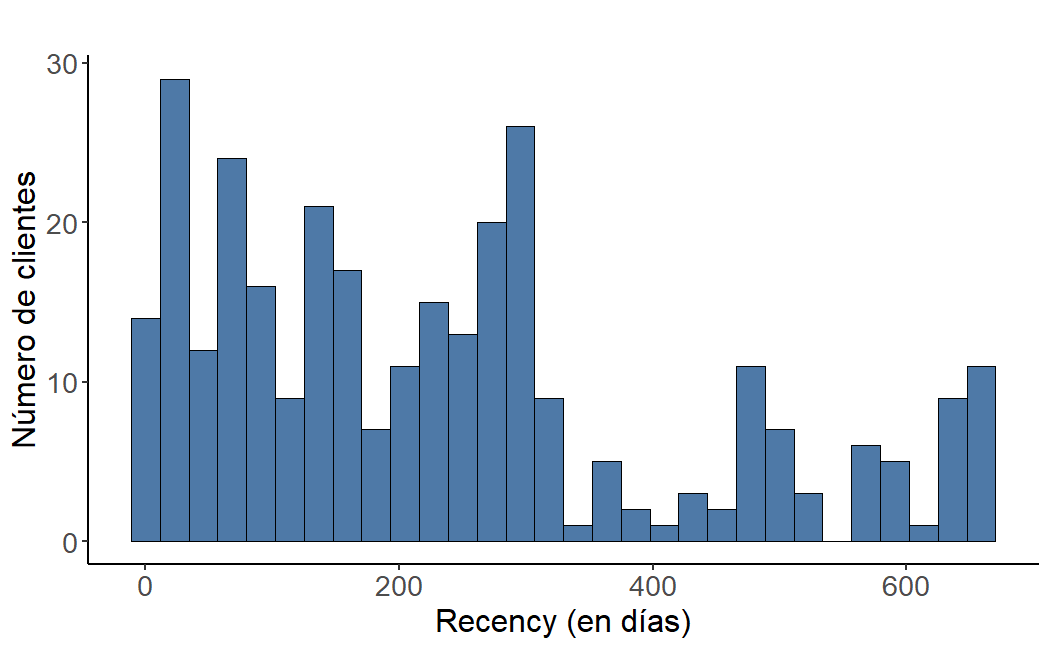
\includegraphics[width=\textwidth]{figuras/Recency.png}
    \caption{Histograma}
    \label{fig:recency_histograma}
\end{subfigure}
\hspace{0.01\textwidth} 
\begin{subfigure}[b]{0.47\textwidth}
    \centering
    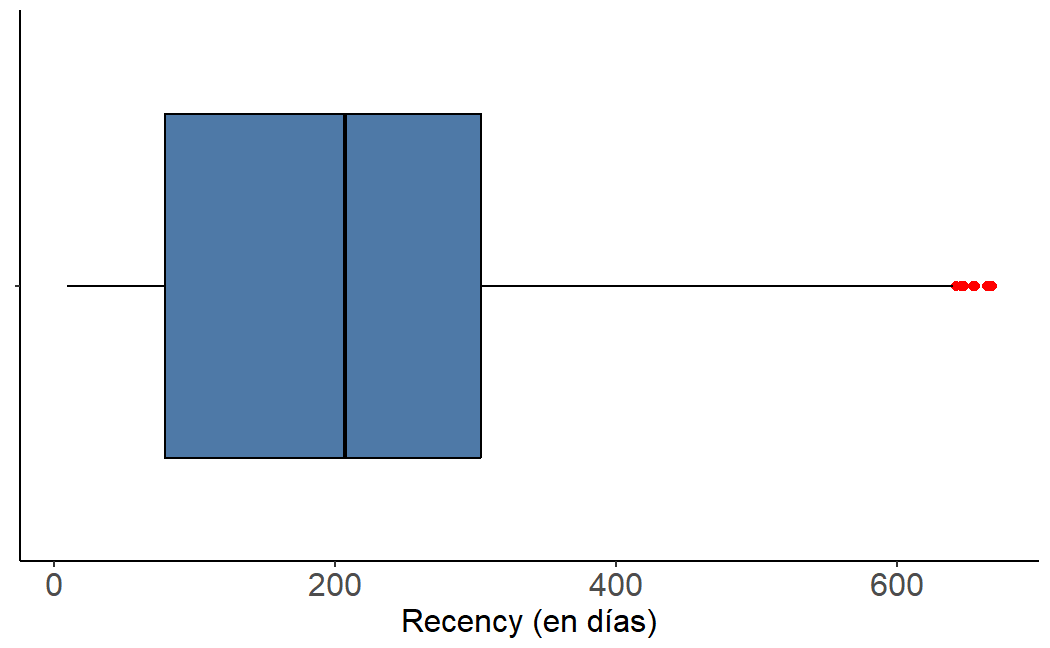
\includegraphics[width=\textwidth]{figuras/Boxplot Recency.png}
    \caption{Boxplot}
    \label{fig:boxplot_recency}
\end{subfigure}
\caption{Distribución de recency}
\label{fig:recency_boxplot_hist}
\end{figure}
\subsubsection{Frequency}
\begin{figure}[H]
\centering
\begin{subfigure}[b]{0.47\textwidth}
    \centering
    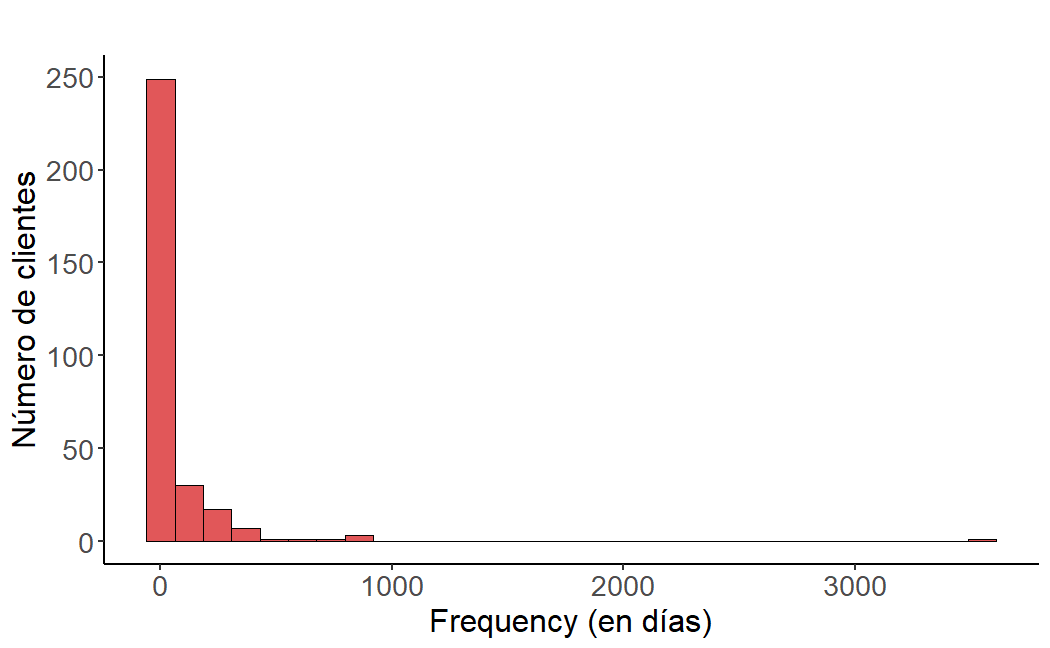
\includegraphics[width=\textwidth]{figuras/Frequency.png}
    \caption{Histograma}
    \label{fig:frequency_histograma}
\end{subfigure}
\hspace{0.01\textwidth}
\begin{subfigure}[b]{0.47\textwidth}
    \centering
    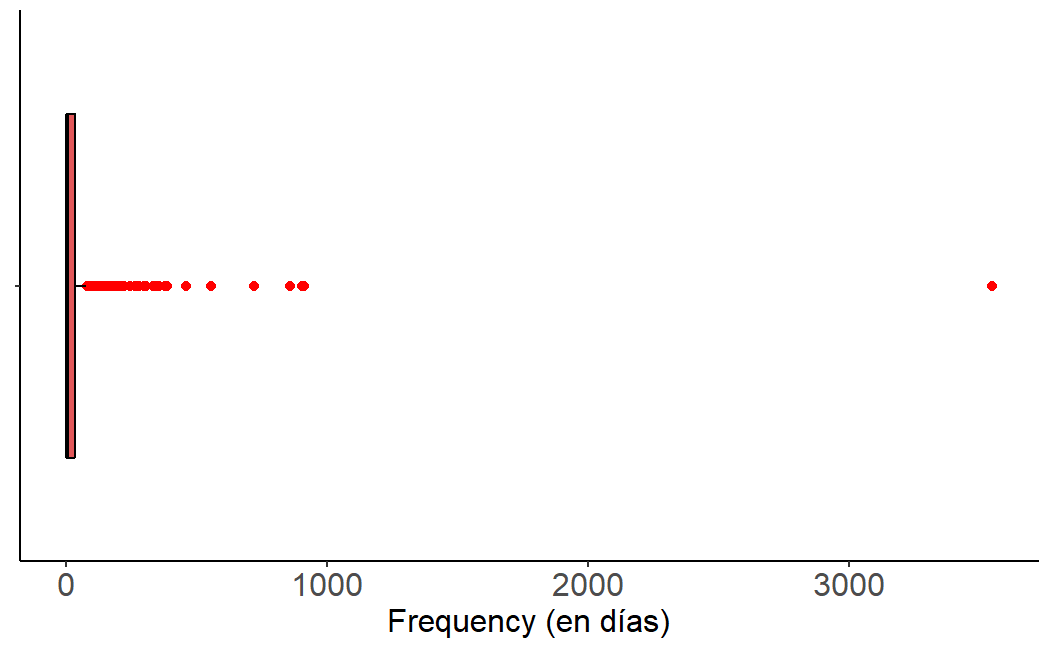
\includegraphics[width=\textwidth]{figuras/Boxplot_Frequency.png}
    \caption{Boxplot}
    \label{fig:frequency_boxplot}
\end{subfigure}
\caption{Distribución de frequency}
\label{fig:recency_boxplot}
\end{figure}

\subsubsection{Monetary}
\begin{figure}[H]
\centering
\begin{subfigure}[b]{0.47\textwidth}
    \centering
    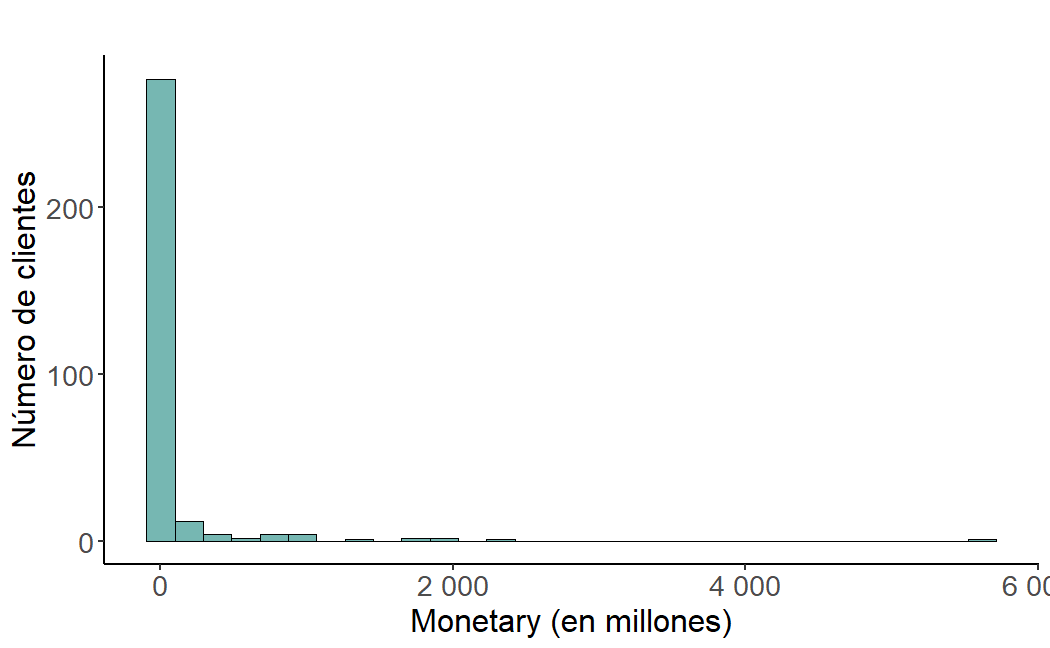
\includegraphics[width=\textwidth]{figuras/Monetary.png}
    \caption{Histograma}
    \label{fig:Histograma_Monetary}
\end{subfigure}
\hspace{0.01\textwidth}
\begin{subfigure}[b]{0.47\textwidth}
    \centering
    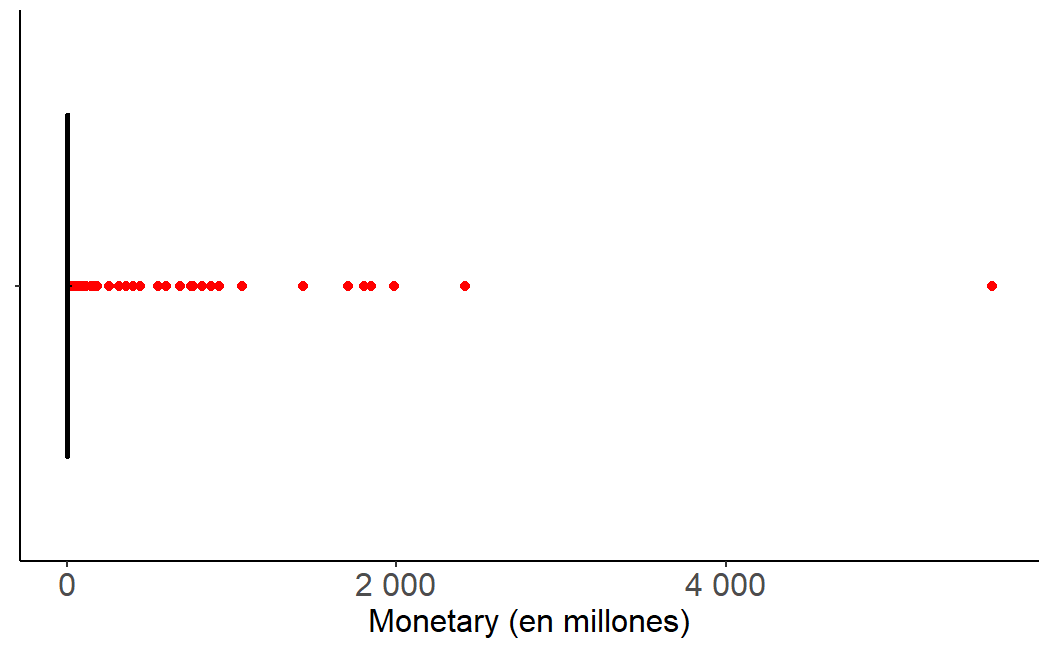
\includegraphics[width=\textwidth]{figuras/Boplot_Monetary.png}
    \caption{Boxplot}
    \label{fig:boxplotmonetary}
\end{subfigure}
\caption{Distribución de monetary}
\label{fig:monetary}
\end{figure}

\subsubsection{Valor Neto}
\begin{figure}[H]
\centering
\begin{subfigure}[b]{0.47\textwidth}
    \centering
    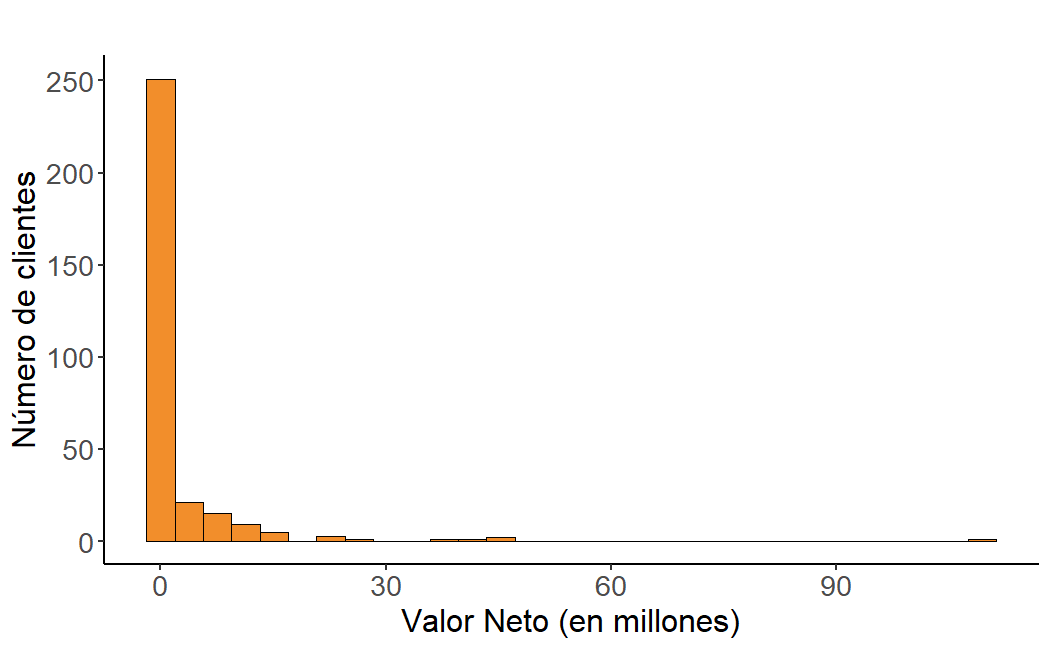
\includegraphics[width=\textwidth]{figuras/Valor Neto.png}
    \caption{Histograma }
    \label{fig:Histograma_Valor Neto}
\end{subfigure}
\hspace{0.01\textwidth}
\begin{subfigure}[b]{0.47\textwidth}
    \centering
    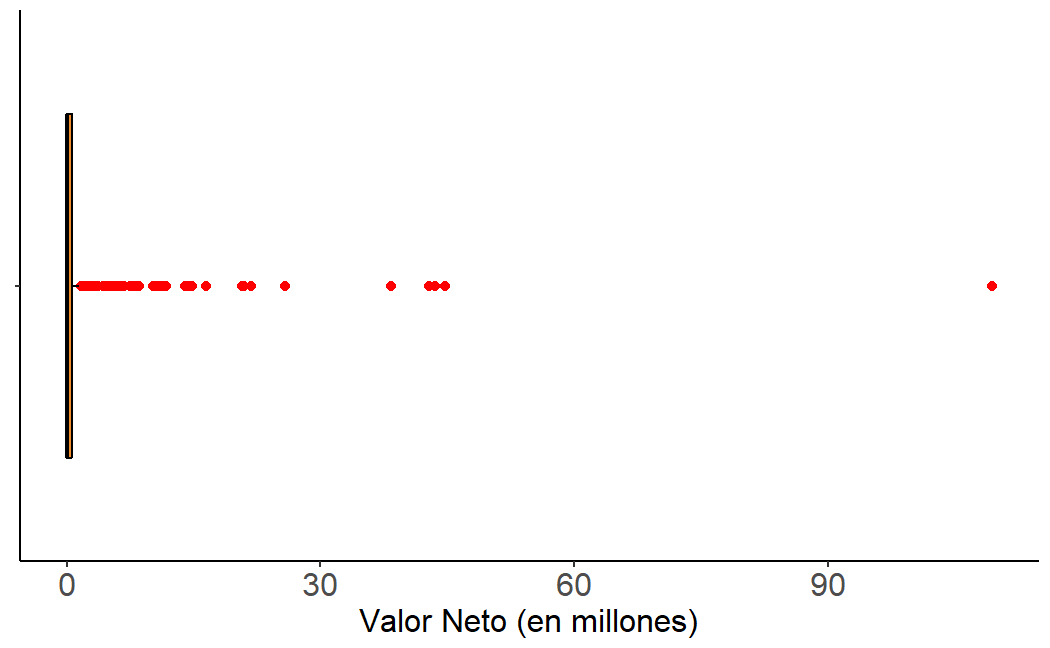
\includegraphics[width=\textwidth]{figuras/Boxplot Valor Neto.png}
    \caption{Boxplot}
    \label{fig:boxplotvalorneto}
\end{subfigure}
\caption{Distribución de la variable valor neto}
\label{fig:valor neto}
\end{figure}

\subsubsection{Valor Bruto}
\begin{figure}[H]
\centering
\begin{subfigure}[b]{0.47\textwidth}
    \centering
    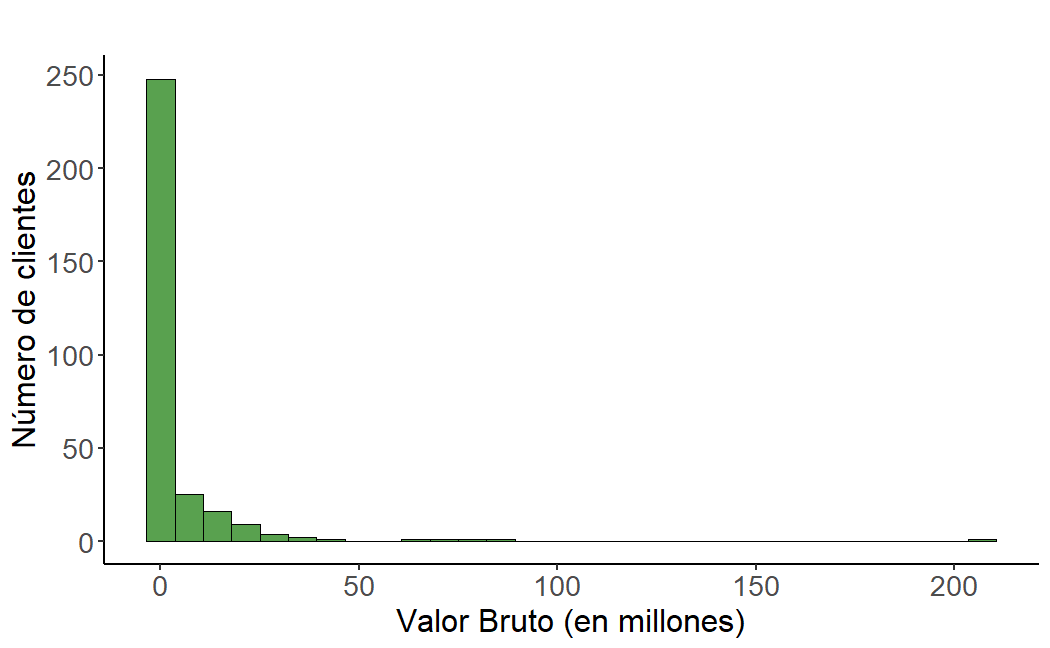
\includegraphics[width=\textwidth]{figuras/Histograma Valor Bruto.png}
    \caption{Histograma}
    \label{fig:Histograma_Valor Bruto}
\end{subfigure}
\hspace{0.01\textwidth}
\begin{subfigure}[b]{0.47\textwidth}
    \centering
    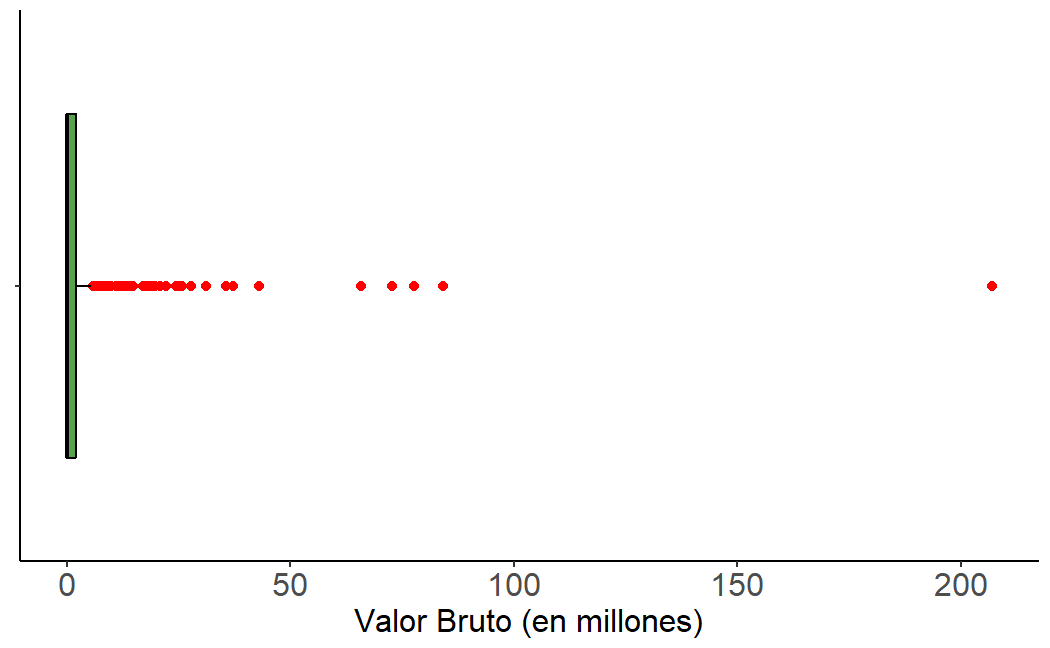
\includegraphics[width=\textwidth]{figuras/Boxplot Valor Bruto.png}
    \caption{Boxplot}
    \label{fig:boxplotvalorbruto}
\end{subfigure}
\caption{Distribución del valor bruto}
\label{fig:valor bruto}
\end{figure}

\subsubsection{Costo Total}
\begin{figure}[H]
\centering
\begin{subfigure}[b]{0.47\textwidth}
    \centering
    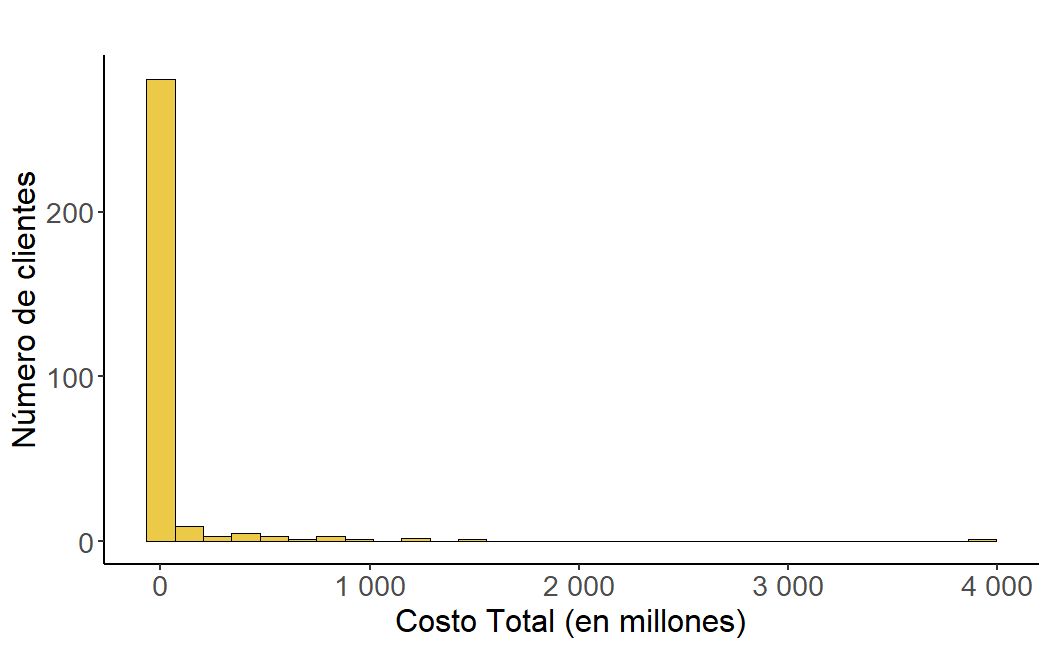
\includegraphics[width=\textwidth]{figuras/Histograma - Costo Total.png}
    \caption{Histograma}
    \label{fig:Histograma_Costo Total}
\end{subfigure}
\hspace{0.01\textwidth}
\begin{subfigure}[b]{0.47\textwidth}
    \centering
    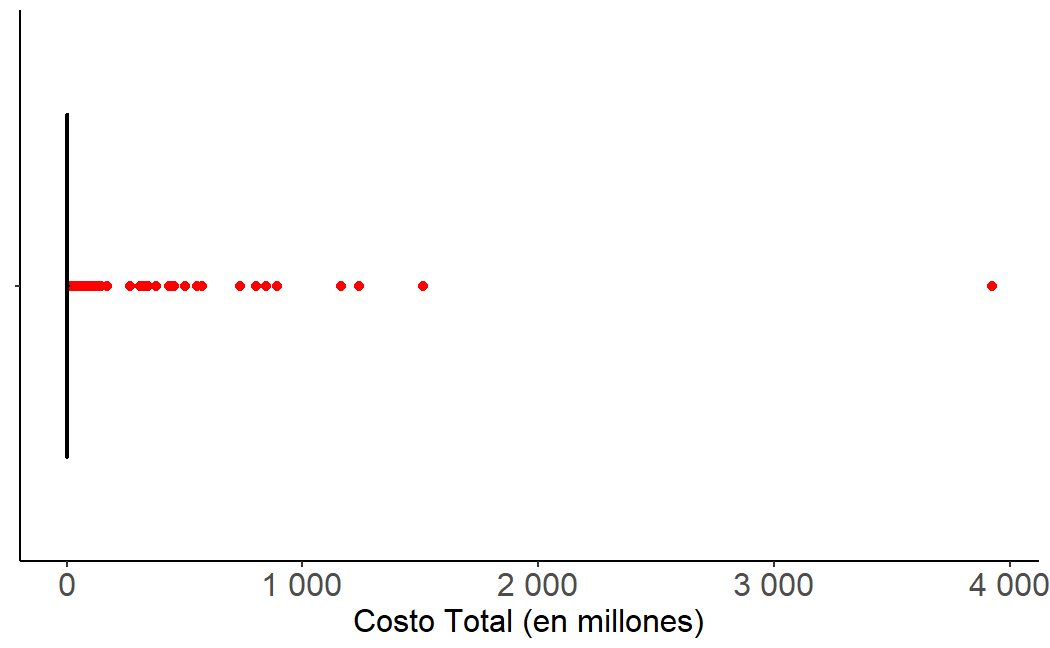
\includegraphics[width=\textwidth]{figuras/Boxplot - Costo Total.png}
    \caption{Boxplot}
    \label{fig:boxplotcostotal}
\end{subfigure}
\caption{Distribución del costo total}
\label{fig:costo total}
\end{figure}

\subsubsection{Cantidad}
\begin{figure}[H]
\centering
\begin{subfigure}[b]{0.47\textwidth}
    \centering
    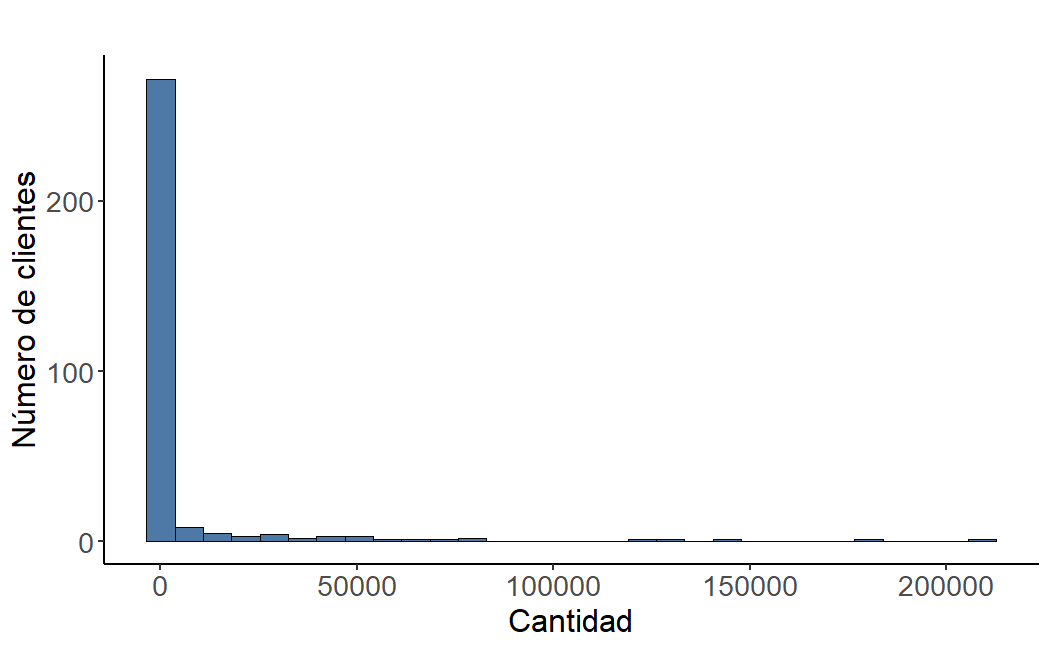
\includegraphics[width=\textwidth]{figuras/Histograma Cantidad.png}
    \caption{Histograma}
    \label{fig:Histograma_Cantidad}
\end{subfigure}
\hspace{0.01\textwidth}
\begin{subfigure}[b]{0.47\textwidth}
    \centering
    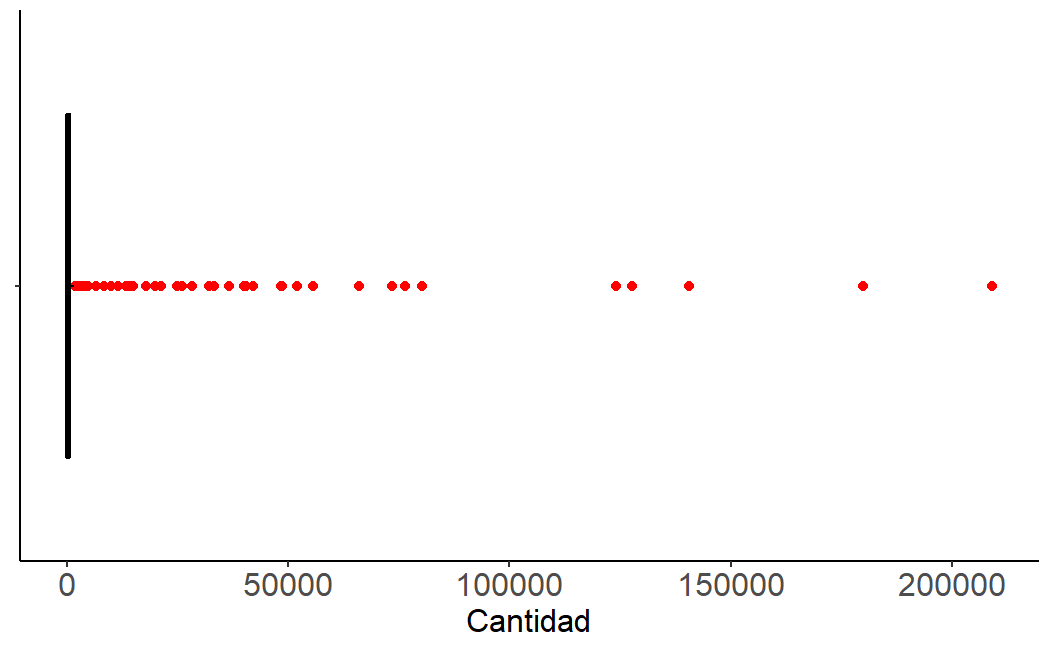
\includegraphics[width=\textwidth]{figuras/Boxplot - Cantidad.png}
    \caption{Boxplot}
    \label{fig:boxplotcantidad}
\end{subfigure}
\caption{Distribución de la variable cantidad}
\label{fig:cantidad}
\end{figure}

\subsubsection{Descuentos}
\label{sec:variablesdescuentos}
\begin{figure}[H]
\centering
\begin{subfigure}[b]{0.47\textwidth}
    \centering
    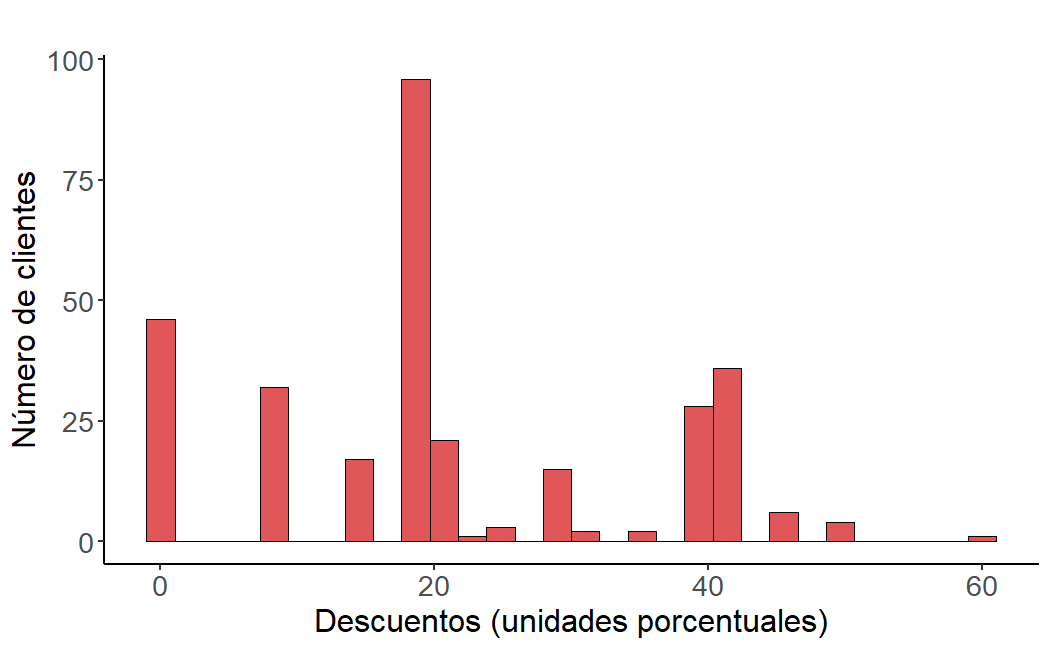
\includegraphics[width=\textwidth]{figuras/Histograma - Descuentos.png}
    \caption{Histograma}
    \label{fig:Histograma_Descuentos}
\end{subfigure}
\hspace{0.01\textwidth}
\begin{subfigure}[b]{0.47\textwidth}
    \centering
    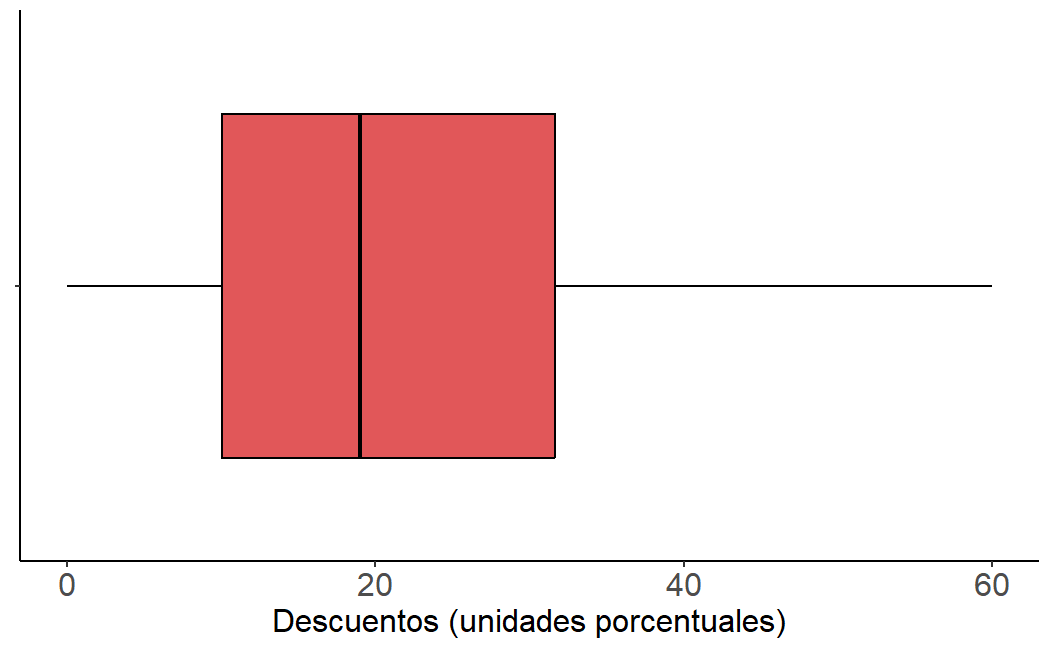
\includegraphics[width=\textwidth]{figuras/Boxplot Descuentos.png}
    \caption{Boxplot}
    \label{fig:boxplotdescuentos}
\end{subfigure}
\caption{Distribución del descuentos}
\label{fig:descuentos}
\end{figure}

\subsubsection{Skus distintos}
\begin{figure}[H]
\centering
\begin{subfigure}[b]{0.47\textwidth}
    \centering
    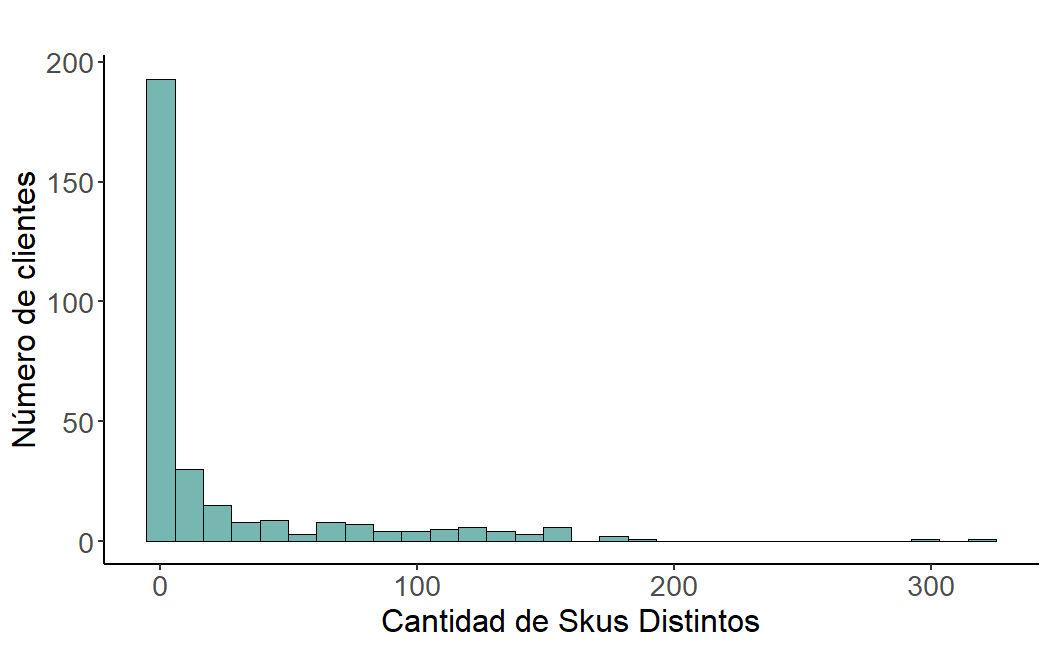
\includegraphics[width=\textwidth]{figuras/Histograma - Skus distintos.png}
    \caption{Histograma}
    \label{fig:Histograma_Skus distintos}
\end{subfigure}
\hspace{0.01\textwidth}
\begin{subfigure}[b]{0.47\textwidth}
    \centering
    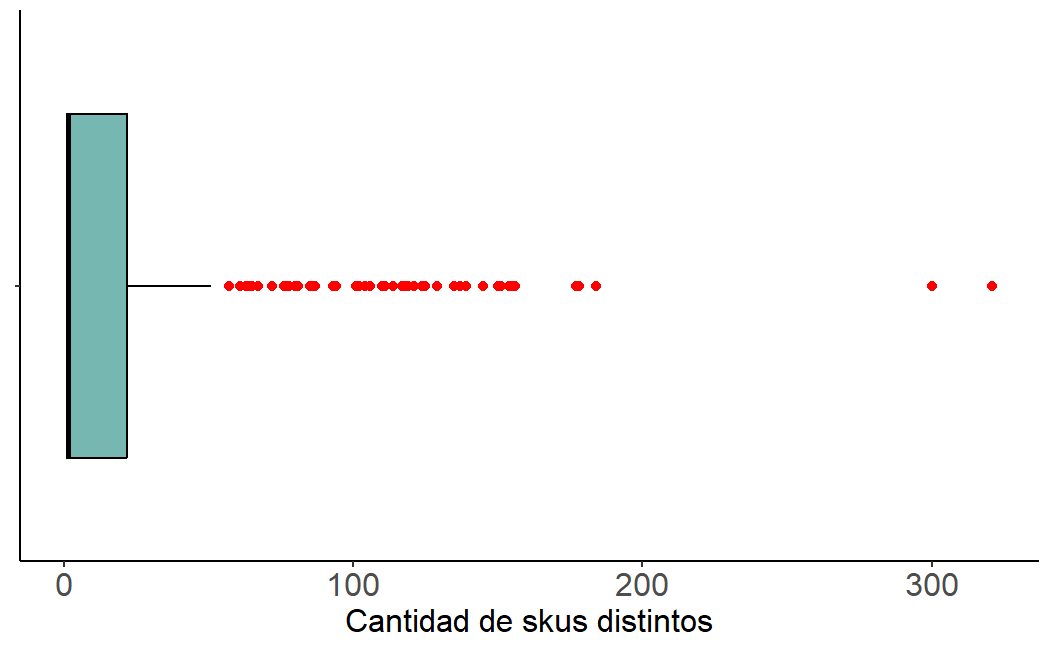
\includegraphics[width=\textwidth]{figuras/Boxplot - Skus Distintos.png}
    \caption{Boxplot}
    \label{fig:boxplotskusdistintos}
\end{subfigure}
\caption{Distribución del número de Skus distintos}
\label{fig:skusdistintos}
\end{figure}
\subsection{Análisis multivariado}
\subsubsection{Matriz de correlación Spearman - variables cuantitativas}
\begin{figure}[H]
\centering
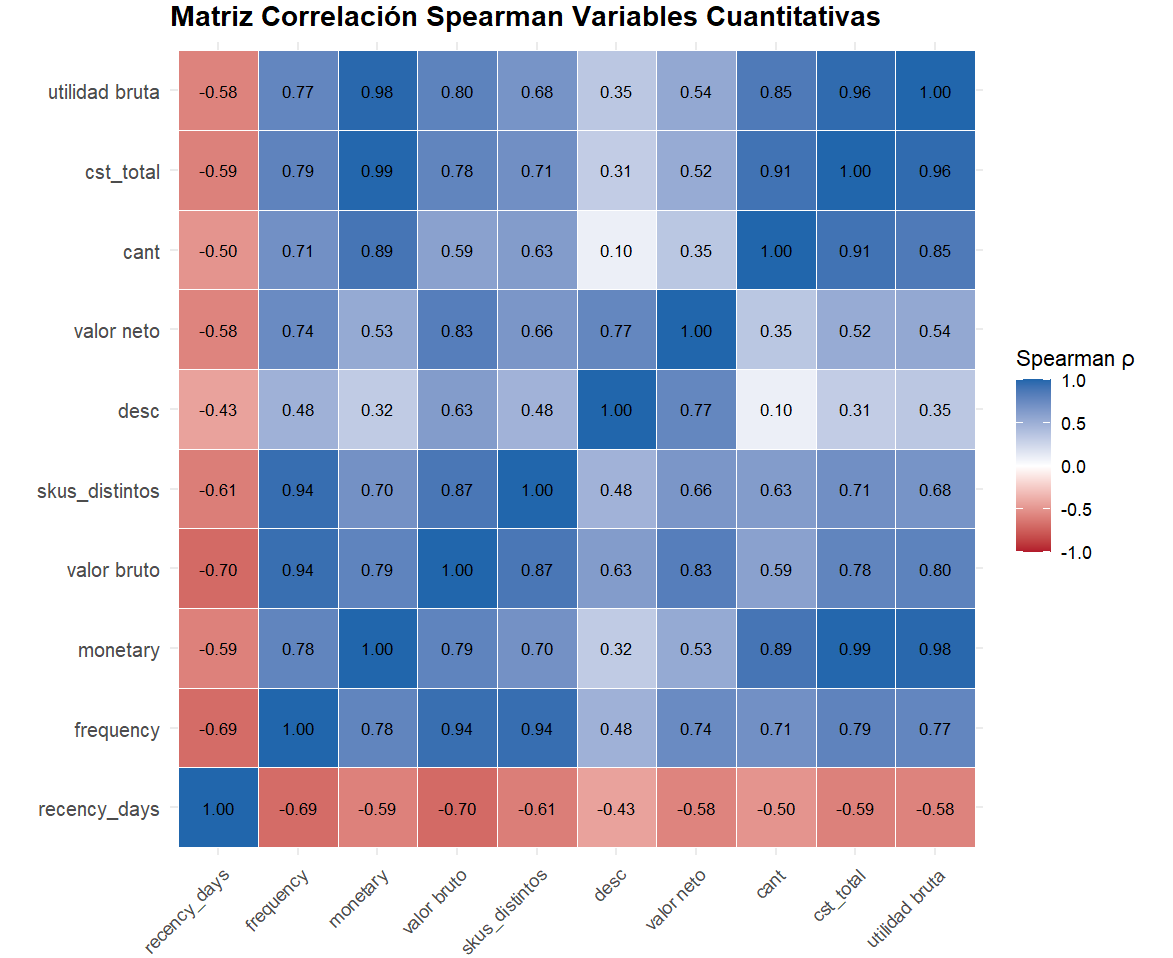
\includegraphics[width=0.8\textwidth]{figuras/CORR_CUANT.png}
\caption{Correlación Spearman Variables Cuantitativas.}
\label{fig:corr_cuantitativas} 
\end{figure}
\subsubsection{Matriz de correlación Cramer - variables cualitativas}
\begin{figure}[H]
\centering
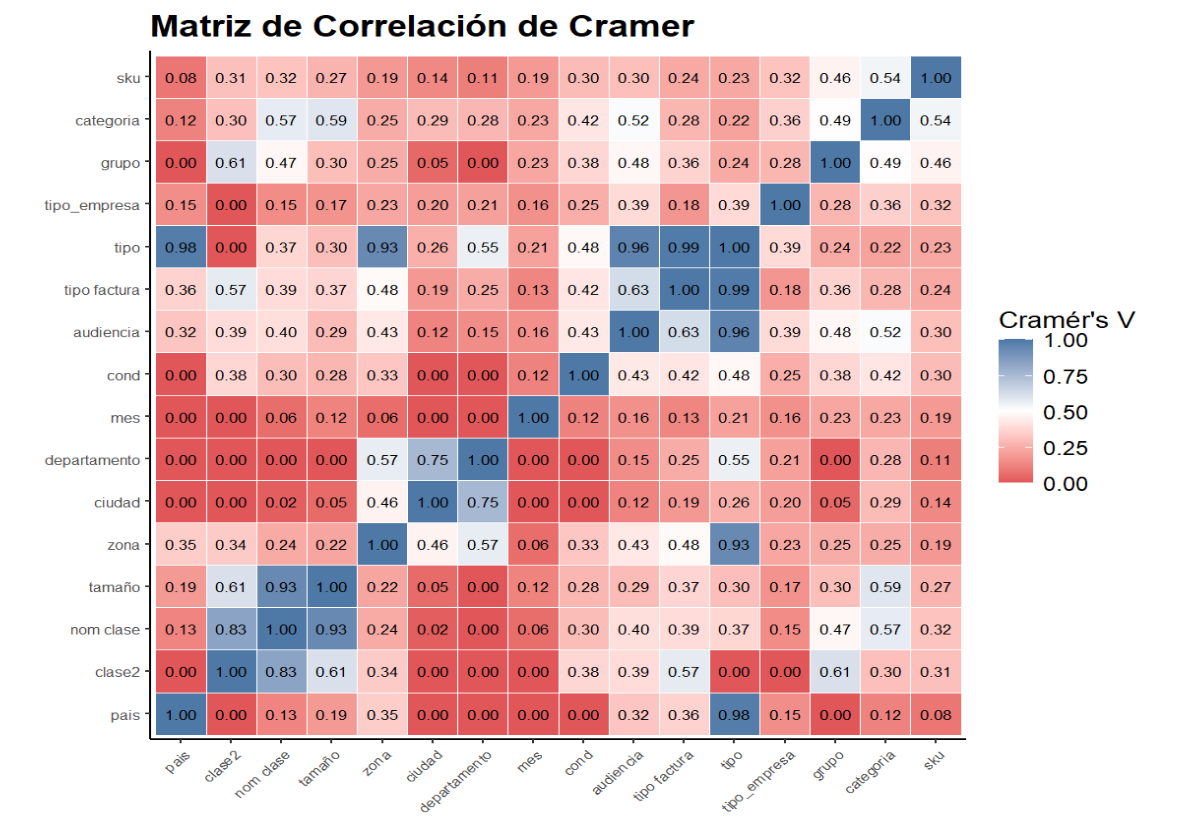
\includegraphics[width=\linewidth]{figuras/Cramer.png} % o \textwidth
\caption{\label{figCramer}Correlación Cramer - variables cualitativas.}
\end{figure}

\clearpage
\printbibliography
    \end{appendices}

    % glossary, bibliography, acknowledges
    %\backmatter
\end{document}